%%%%%%%%%%%%%%%%%%%%%%%%%%%%%%%%%%%%%%%%%%%%%%%%%%%
%
%  New template code for TAMU Theses and Dissertations starting Fall 2012.  
%  For more info about this template or the 
%  TAMU LaTeX User's Group, see http://www.howdy.me/.
%
%  Author: Wendy Lynn Turner 
%	 Version 1.0 
%  Last updated 8/5/2012
%
%%%%%%%%%%%%%%%%%%%%%%%%%%%%%%%%%%%%%%%%%%%%%%%%%%%

%%%%%%%%%%%%%%%%%%%%%%%%%%%%%%%%%%%%%%%%%%%%%%%%%%%%%%%%%%%%%%%%%%%%%%
%%                           SECTION 4
%%%%%%%%%%%%%%%%%%%%%%%%%%%%%%%%%%%%%%%%%%%%%%%%%%%%%%%%%%%%%%%%%%%%%%

%%%%%%%%%%%%%%%%%%%%%%%%%%%%%%%%%%%%%%%%%%%%%%%%%%%%%%%%%%%%%%%%%%%%%%%
\chapter{\uppercase {Application of the entropy viscosity method to the seven-equation model}}\label{chap:seven}
%%%%%%%%%%%%%%%%%%%%%%%%%%%%%%%%%%%%%%%%%%%%%%%%%%%%%%%%%%%%%%%%%%%%%%
%
Compressible two-phase flows are found in numerous industrial applications and are an ongoing area of research in modeling and simulation over many years. A variety of models with different levels of complexity has been developed such as: five-equation model \cite{Kapila_2001}, six-equation model \cite{Toumi_1996}, and more recently the seven-equation model \cite{SEM}. These models are all obtained by integrating the single-phase flow balance equations weighed by a characteristic or indicator function for each phase. The resulting system of equations contains non-conservative terms that describe the interaction between phases but also an equation for the volume fraction. Once a system of equations describing the physics is derived, the next challenging step is to develop a robust and accurate discretization to obtain a numerical solution. Assuming that the system of equations is hyperbolic under some conditions, a Riemann solver could be used but is often ruled out because of the complexity due to the number of equations involved. Furthermore, careless approximation for the treatment of the non-conservative terms can lead to failure in computing the numerical solution \cite{Abgrall_2002}. An alternative is to use an approximate Riemann solver, a well-established approach for single-phase flows, while deriving a consistent discretization scheme for the non-conservative terms. 

This methodology was applied to the seven-equation model (SEM) introduced by Berry et al. in \cite{SEM}. This model is known to be unconditionally hyperbolic which is highly desirable when working with approximate Riemann solvers and can treat a wide range of applications. Its particularity comes from the pressure and velocity relaxation terms in the volume fraction, momentum and energy equations that can bring the two phases in equilibrium when using large values of the relaxation parameters. In other words, the seven-equation model can degenerate into the six- and five-equation models. Alike for the other two-phase flow models, solving for the seven-equation model requires a numerical solver and significant effort was dedicated to this task for spatially discontinuous schemes. Because each phase is assumed to obey the Euler equations, most of the numerical solvers are adapted from the single-phase approximate Riemann solvers. For example, Saurel et al. \cite{Saurel_2001a, Saurel_2001b} employed a HLL-type scheme to solve for the SEM but noted that excessive dissipation was added to the contact discontinuity. A more advanced HLLC-type scheme was developed in \cite{Li_2004} but only for the subsonic case and then extended to supersonic flows in \cite{Zein_2010}. More recently, Ambroso et al. \cite{Ambroso_2012} proposed an approximate Riemann solver accounting for source terms such as gravity and drag forces, but with no interphase mass transfer.

We propose to investigate how the EVM applies to the seven-equation model when discretized with a CFEM. First, the multi-D seven-equation model is recalled and detailed in \sect{sec:multi-seven-equ-model} and particular attention is given to the entropy equation. Then, the dissipative terms are derived using the entropy inequality, in \sect{sec:sev-equ-visc-reg-sect4}, on the same principle of what was done in \chap{chap:euler} for the multi-D Euler equations. In \sect{sec:sev-equ-visc-coeff-sect4}, a low-Mach asymptotic limit is performed in order to derive a definition for the viscosity coefficients consistent with the incompressible limit results. Lastly, 1-D numerical results are presented in \sect{sec:1d-num-res-sect4}.
%\begin{itemize}
%\item background on 7 emu model: first introduced. 
%\item method to solve this system: discontinuous scheme. Approximate Riemann solvers. Quote several papers
%\item differences between system of equation -> closure relations for relaxation coefficients.
%\end{itemize}

%===================================================================================
\section{Descriptions of the multi-D seven-equation model}\label{sec:multi-seven-equ-model}
%===================================================================================

The multi-D seven-equation model is obtained by assuming that each phase obeys the single-phase Euler equations (with phase-exchange terms) and by integrating over a control volume after multiplying by a characteristic function. The detailed derivation can be found in \cite{SEM}. In this section, the governing equations are recalled for each phase (liquid and vapor) and the source terms are described. 
%-----------------------------------------------------------------------------------------
\subsection{The system of equations for the liquid and vapor phases}\label{sec:multi-d-7eqn-model-sect4}
%-----------------------------------------------------------------------------------------
The liquid phase obeys the following mass, momentum and energy balance equations, supplemented by a non-conservative volume-fraction equation:
%
\begin{subequations}\label{eq:liq-7-eqn-sect5}
\begin{align}
  % liquid mass conservation
  \label{multi-d-7-equ-liq}
  \frac{\partial \left( \alpha \rho \right)_{liq} A}{\partial t}
  + \div \left( \alpha \rho \mbold u A\right)_{liq}
  &= - \Gamma A_{int} A
\end{align}
\begin{align}
  % liquid momentum
  \frac{\partial \left( \alpha \rho \mbold u \right)_{liq} A}{\partial t}
  + \div \left[ \alpha_{liq} A \left( \rho \mbold u \otimes \mbold u + P \mathbb{I} \right)_{liq} \right]
  &= P_{int} A \grad \alpha_{liq} + P_{liq} \alpha_{liq} \grad A
    \nonumber
  \\
  &+ A \lambda_u (\mbold u_{vap} - \mbold u_{liq})
  - \Gamma A_{int} \mbold u_{int} A
\end{align}
\begin{align}
  % liquid total energy
  \frac{\partial \left( \alpha \rho E \right)_{liq} A}{\partial t}
  + \div \left[ \alpha_{liq} \mbold u_{liq} A \left( \rho E + P \right)_{liq} \right]
  &= P_{int} \mbold u_{int} A \grad \alpha_{liq} - \bar{P}_{int} A \mu_P (P_{liq} - P_{vap})
        \nonumber
  \\
  + \bar{\mbold u}_{int} A \lambda_u (\mbold u_{vap} - \mbold u_{liq})
&  + \Gamma A_{int} \left( \frac{P_{int}}{\rho_{int}} - H_{liq, int} \right) A
\nonumber 
\\
& + Q_{wall,liq} + Q_{int,liq}
\end{align}
\begin{align}
  % liquid volume fraction
  \label{eqn:multi-d-7-eqn-liq-vol}
  \frac{\partial \alpha_{liq} A}{\partial t} + A\mbold u_{int} \cdot \grad \alpha_{liq}
  &= A \mu_P (P_{liq} - P_{vap}) - \frac{\Gamma A_{int} A}{\rho_{int}}
\end{align}
\end{subequations}
%
On the same model, the equations for the vapor phase are:
%
\begin{subequations}\label{eq:vap-7-eqn-sect5}
\begin{align}
  \label{multi-d-7-equ-vap}
  % vapor mass conservation
  \frac{\partial \left( \alpha \rho A\right)_{vap}}{\partial t}
  + \div \left( \alpha \rho \mbold u \right)_{vap} A
  =  \Gamma A_{int} A
\end{align}
\begin{align}
  % vapor momentum
  \frac{\partial \left( \alpha \rho u \right)_{vap} A}{\partial t}
  + \div \left[ \alpha_{vap} A \left( \rho \mbold u \otimes \mbold u + P\mathbb{I} \right)_{vap} \right]
  &= P_{int} A \grad \alpha_{vap} + P_{vap} \alpha_{vap} \grad A
  \\
  \nonumber
  &+ A \lambda_u (\mbold u_{liq} - \mbold u_{vap})
  + \Gamma A_{int} u_{int} A
\end{align}
\begin{align}
  % vapor total energy
  \frac{\partial \left( \alpha \rho E \right)_{vap} A}{\partial t}
  + \div \left[ \alpha_{vap} \mbold u_{vap} A \left( \rho E + P \right)_{vap} \right]
  &= P_{int} \mbold u_{int} A \grad \alpha_{vap} - \bar{P}_{int} A \mu_P (P_{vap} - P_{liq})
    \nonumber
  \\
  + \bar{\mbold u}_{int} A \lambda_u (\mbold u_{liq} - \mbold u_{vap})
&- \Gamma A_{int} \left( \frac{P_{int}}{\rho_{int}} - H_{vap, int} \right) A
\nonumber 
\\
& + Q_{wall,vap} + Q_{int,vap}
\end{align}
\begin{align}
  % vapor phase volume fraction
  \label{eqn:multi-d-7-eqn-vap-vol}
  \frac{\partial \alpha_{vap} A}{\partial t} + A \mbold u_{int} \cdot \grad \alpha_{vap}
  &= A \mu_P (P_{vap} - P_{liq}) + \frac{\Gamma A_{int} A}{\rho_{int}}
\end{align}
\end{subequations}
%
where $\alpha_k$, $\rho_k$, $\mbold u_k$ and $E_k$ denote the volume fraction, the density, the velocity vector and the total specific energy of phase $k=\left\{ liq, vap \right\}$, respectively. The phase pressure $P_k$ is computed from an equation of state. The interfacial variables are denoted by the subscript $int$ and their definition will be given in \sect{sec:source-terms-7-eqt-sect5}. The interfacial pressure and velocity and their corresponding average values are denoted by $P_{int}$, $\mbold u_{int}$, $\bar{P}_{int}$ and $\bar{\mbold u}_{int}$, respectively. $\Gamma$ is the net mass transfer rate per unit interfacial area from the liquid to the vapor phase and $A_{int}$ is the interfacial area per unit volume of mixture.  Also, $H_{liq, int}$ and $H_{vap, int}$ are the liquid and gas total specific enthalpies at the interface, respectively, with the following definition: $H_k = h_k + 0.5 || \mbold u ||^2$. $\mu_P$ is the pressure relaxation coefficient and $\lambda_u$ denotes the velocity relaxation coefficient. The wall and interfacial heat sources are denoted by $Q_{wall,k}$ and $Q_{int,k}$, respectively, and are detailed in \sect{sec:source-terms-7-eqt-sect5}. Lastly, the cross section $A$ is assumed spatially dependent. In the case of two-phase flows, the equation for the vapor volume fraction, \eqt{eqn:multi-d-7-eqn-vap-vol}, is simply replaced by the algebraic relation
%
\begin{align}
 \alpha_{vap}= 1 - \alpha_{liq}
\end{align}
%
The set of eight equations given in \eqt{eq:liq-7-eqn-sect5} and in \eqt{eq:vap-7-eqn-sect5} is now reduced to seven which yields the multi-D seven-equation model. A set of seven waves is present in such a model: two acoustic waves and a contact wave for each phase supplanted by a volume fraction wave propagating at the interfacial velocity $\mbold u_{int}$. Considering a domain of dimension $\mathbb{D}$, the corresponding eigenvalues are the following for each phase $k$:
% 
\begin{align}
&\lambda_1 = \mbold u_{int} \cdot \bar{\mbold n} \nonumber\\
&\lambda_{2,k} = \mbold u_k \cdot \bar{\mbold n} - c_k \nonumber\\
&\lambda_{3,k} = \mbold u_k \cdot \bar{\mbold n} + c_k \nonumber\\
&\lambda_{d+3,k} = \mbold u_k \cdot \bar{\mbold n} \text{ for } d = 1 \dots \mathbb{D},\nonumber
\end{align}
%
where $\bar{\mbold n}$ is a unit vector pointing to a given direction.
For each phase $k$, an entropy equation can be derived when accounting only for the pressure and velocity relaxation terms (all of the terms proportional to the net mass transfer term $\Gamma$ and the interfacial heat transfer $Q_{int,k}$ are removed). The entropy function for a phase $k$ is denoted by $s_k$ and function of the density $\rho_k$ and the internal energy $e_k$. The derivation is detailed in \app{app:sev-equ-model-entropy} and only the final result is recalled here when assuming that the phase $k$ is in interaction with a phase $j$:
%
\begin{align}\label{eq:ent-eqn-7-eqn-model}
(s_{e})_k^{-1} \alpha_k \rho_k A \frac{Ds_k}{Dt} &= \mu_P \frac{Z_k}{Z_k+Z_j} (P_j - P_k)^2 + \lambda_u \frac{Z_j}{Z_k+Z_j} (\mbold u_j -\mbold  u_k)^2 \nonumber
\\
& \frac{Z_k}{\left( Z_k+Z_j \right)^2} \left[ Z_j (\mbold u_j-\mbold u_k)+\frac{\grad \alpha_k}{|| \grad \alpha_k ||}(P_k-P_j)\right]^2,
\end{align}
where $Z_{k}$ denotes the phasic acoustic impedance and is defined as the product of the density and the speed of sound: $Z_k = \rho_k c_k$. The partial derivative of the entropy function $s_k$ with respect to the internal energy $e_k$, $(s_e)_k$, is defined proportional to the inverse of the temperature of phase $k$ as in \chap{chap:euler} for the single phase Euler equations. The right hand-side of \eqt{eq:ent-eqn-7-eqn-model} is unconditionally positive since all terms are squared. Furthermore, \eqt{eq:ent-eqn-7-eqn-model} is valid for each phase $k=\left\{liq, vap \right\}$ and ensures positivity of the total entropy equation that is obtained by summing over the phases:
%
\begin{equation}\label{eq:tot-ent-res-sct4}
\sum_k (s_{e})_k^{-1} \alpha_k \rho_k A \frac{Ds_k}{Dt} = \sum_k (s_{e})_k^{-1} \alpha_k \rho_k A \left( \partial_t s_k + \mbold u_k \cdot \grad s_k \right) \geq 0.
\end{equation}
%
Note that when one phase disappears, \eqt{eq:tot-ent-res-sct4} degenerates into the single phase entropy equation given in \eqt{eq:ent_res}.
%\begin{itemize}
%\item give system of equation with relaxation terms and mass transfer term from DEM paper
%\item explain the relaxation terms
%\item explain the source terms: exchanges between phases.
%\item entropie equation.
%\end{itemize}
%-----------------------------------------------------------------------------------------
\subsection{The source terms}\label{sec:source-terms-7-eqt-sect5}
%-----------------------------------------------------------------------------------------
In this section, insights about the relaxation terms, the net mass transfer term and the interfacial heat transfer terms are given.
%---------------------------------------------------------------------------------------------------------------
\subsubsection{Interface pressure and velocity, mechanical relaxation coefficients}
%---------------------------------------------------------------------------------------------------------------
The mechanical relaxation terms are used to bring the two phases into equilibrium by making pressure and velocity equal. The mechanical relaxation coefficients $\mu_P$ and $\lambda_u$ can be seen as inverse relaxation times: the larger the relaxation coefficients, the faster the two phases will be brought to equilibrium. Derivation of the relaxation terms is achieved by using rational thermodynamic to ensure consistency with the second thermodynamic law for the two-phase mixture \cite{Truesdell}. The methodology is very similar to what is done for the derivation of the dissipative terms using the entropy inequality.

In the continuous limit of small mesh spacing and time steps along with employment of the Godunov weak wave limit, it can be shown that the pressure and velocity relaxation terms obeys the following relations \cite{Berry_2008b, Chinnayya_2004}:
%
\begin{align}
  \label{E-R:83}
  P_{int} &= \bar{P}_{int} + \frac{Z_{liq}Z_{vap}}{Z_{liq}+Z_{vap}} \frac{\grad \alpha_{liq}}{|| \grad \alpha_{liq} ||} \cdot (\mbold u_{vap}-\mbold u_{liq})
  \\
  \bar{P}_{int} &= \frac{Z_{vap}P_{liq}+Z_{liq}P_{vap}}{Z_{liq}+Z_{vap}}
\end{align}
%
The interfacial velocities $\mbold u_{int}$ and its average value $\bar{\mbold u}_{int}$ are computed from:
%
\begin{align}
  \label{E-R:84}
  \mbold u_{int} &= \bar{\mbold u}_{int} +  \frac{\grad \alpha_{liq}}{|| \grad \alpha_{liq} ||} \frac{P_{vap}-P_{liq}}{Z_{liq}+Z_{vap}}
  \\
  \bar{\mbold u}_{int} &= \frac{Z_{liq} \mbold u_{liq}+Z_{vap}\mbold u_{vap}}{Z_{liq}+Z_{vap}}.
\end{align}
%
The pressure, $\mu_P$, and velocity, $\lambda_u$, relaxation coefficients are proportional to each other and function of the interfacial area $A_{int}$:
%
\begin{align}
  \label{E-R:85}
  \lambda_u &= \frac{1}{2} \mu_P Z_{liq} Z_{vap}
  \\
  \label{E-R:86}
  \mu_P &= \frac{A_{int}}{Z_{liq}+Z_{vap}}
\end{align}
%where $\lambda_u$ is the velocity relaxation coefficient function, $\mu_P$
%is the pressure relaxation coefficient function, $Z_k = \rho_k c_k$,
%$(k=liq, vap)$, is the phasic acoustic impedance and 
The specific interfacial area (i.e., the interfacial surface area per unit
volume of two-phase mixture), $A_{int}$, must be specified from some type of
flow regime map or function under the form of a correlation. In \cite{SEM}, $A_{int}$ is chosen to be a function of the liquid volume fraction:
%
\begin{equation}\label{eq:Aint-sect4}
A_{int} = A_{int}^{max} \left[ 6.75 \left(1-\alpha_{liq} \right)^2 \alpha_{liq} \right],
\end{equation}
% 
where $A_{int}^{max} = 5100$ $m^2 / m^3$. With such definition, the interfacial area is zero in the limits $\alpha_{liq} = 0$ and $\alpha_{liq} = 1$. 
%The DEM model for two-phase flow of
%water and its vapor in a one dimensional duct of spatially varying
%cross-section was derived and demonstrated with these closures by
%Berry et al.~\cite{SEM}.
%From this specification for $\lambda_u$ and $\mu_P$ it is clear
%that special coupling is rendered\tcr{???}.  
To relax the seven-equation model to
the ill-posed classical six-equation model, only the pressures should be
relaxed toward a single pressure for both phases.  This is
accomplished by specifying the pressure relaxation coefficient to be
very large, i.e., letting it approach infinity.  But if the pressure
relaxation coefficient goes to infinity, so does the velocity
relaxation rate also approach infinity.  This then relaxes the
seven-equation model not to the classical six-equation model but to the
mechanical equilibrium five-equation model of Kapila \cite{Kapila_2001}.  This reduced
five-equation model is also hyperbolic and well-posed. The five-equation
model provides a very useful starting point for constructing
multi-dimensional interface resolving methods which dynamically
captures evolving and spontaneously generated
interfaces~\cite{Saurel_2009}. Thus the seven-equation model
can be relaxed locally to couple seamlessly with such a
multi-dimensional, interface resolving code.

Numerically, the mechanical relaxation coefficients $\mu_P$
(pressure) and $\lambda_u$ (velocity) can be relaxed independently to
yield solutions to useful, reduced models (as explained previously).  It
is noted, however, that relaxation of pressure only by making $\mu_P$
large without relaxing velocity will indeed give ill-posed and
unstable numerical solutions, just as the classical six-equation
two-phase model does, with sufficiently fine spatial resolution, as
confirmed in~\cite{SEM,Herrard_2005}.

Even though the implementation of the seven-equation two-phase
model does not use
the generalized approach of DEM \cite{SEM}, the interfacial pressure and velocity
closures as well as the pressure and velocity relaxation coefficients
of Equations~\eqref{E-R:83} to~\eqref{E-R:86} are utilized.
%-----------------------------------------------------------------------------------------
\subsubsection{Interphase mass transfer}
%-----------------------------------------------------------------------------------------
For vapor to be formed from the liquid phase (vaporization) energy
must be added to the liquid to produce vapor at nucleation sites;
whether the liquid is heated directly or decompressed below its
saturation pressure.  A liquid to vapor phase change may occur based
on two main mechanisms.  The first is related to vaporization induced
by external heating or heat transfer in a nearly constant pressure
environment which is called heterogeneous boiling, or simply
boiling.  This heat input can occur through a solid/liquid
interface with the solid typically hotter than the liquid, or through
a liquid/gas interface with the gas being hotter than the liquid.

\begin{figure}[H]
  \centering
  %\fbox{
   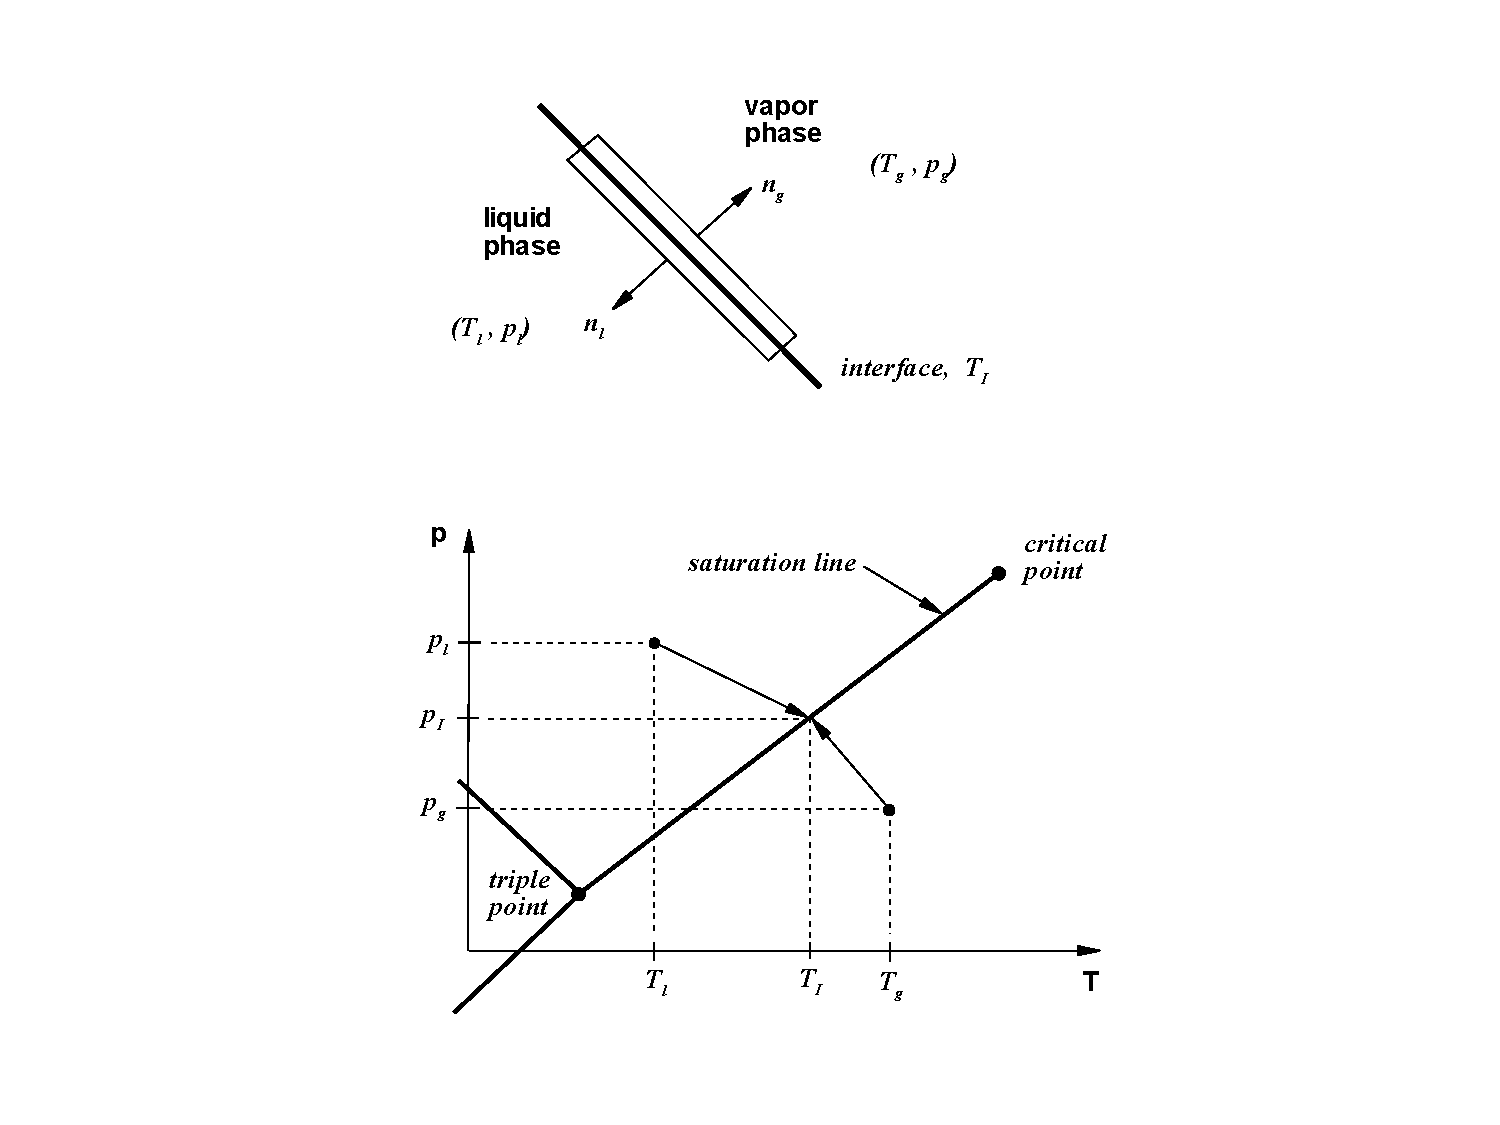
\includegraphics[clip=true,viewport=200 50 550 500,width=.8\textwidth]{figures/SEM/saturation}
   % }
   \caption{Interface control volume (top); $T$-$p$ state space around
     saturation line, $T_{liq} < T_{vap}$, (bottom).\label{Berry-Fig:2}}
\end{figure}

To examine the mass flow rate between phases, local mechanisms of the
vaporization (condensation) process are considered between the liquid
phase and its associated vapor in the presence of temperature
gradients.  The mechanisms of interest here are dominated by heat
diffusion at the interface.  The pertinent local equations to consider
are the mass and energy equations.  As a vaporization front propagates
slowly (on the order of 1 mm/s to 1 m/s) compared to acoustic waves
present in the medium (which propagate with speeds of the order 1
km/s), acoustic propagation results in quasi-isobaric pressure
evolution through vaporization fronts.  The momentum equation is
therefore not needed, because the quasi-isobaric assumption
(neglecting the pressure and kinetic energy variations in the total
energy equation) is made.  A simple expression for the interphase
mass flow rate is obtained from \cite{SEM}:
\begin{align}
  \nonumber
  \Gamma = \Gamma_{vap}
  &= \frac{h_{T,  liq} \left( T_{liq} - T_{int} \right) + h_{T,  vap} \left( T_{vap} - T_{int} \right)}{h_{vap,  int} - h_{liq,  int}}
  \\
  &= \frac{h_{T,  liq} \left( T_{liq} - T_{int} \right) + h_{T,  vap} \left( T_{vap} - T_{int} \right)}{L_v \left( T_{int} \right)}
\end{align}
where $L_v \left( T_{int} \right) = h_{vap,  int} - h_{liq,  int}$
represents the latent heat of vaporization.  The interface
temperature is determined by the saturation constraint
$T_{int}=T_{sat}(P)$ with the appropriate pressure $P=\bar{P}_{int}$
determined above, the interphase mass flow rate is thus determined.
The lower graphic of Figure~\ref{Berry-Fig:2} schematically shows the
$P$-$T$ state space in the vicinity of the saturation line (shown
for the case with $T_{liq} < T_{vap}$).

To better illustrate the model for vaporization or condensation,
Figure~\ref{Berry-Fig:3} shows pure liquid and pure vapor regions
separated by an interface.
\begin{figure}[H]
  \centering
  %\fbox{
   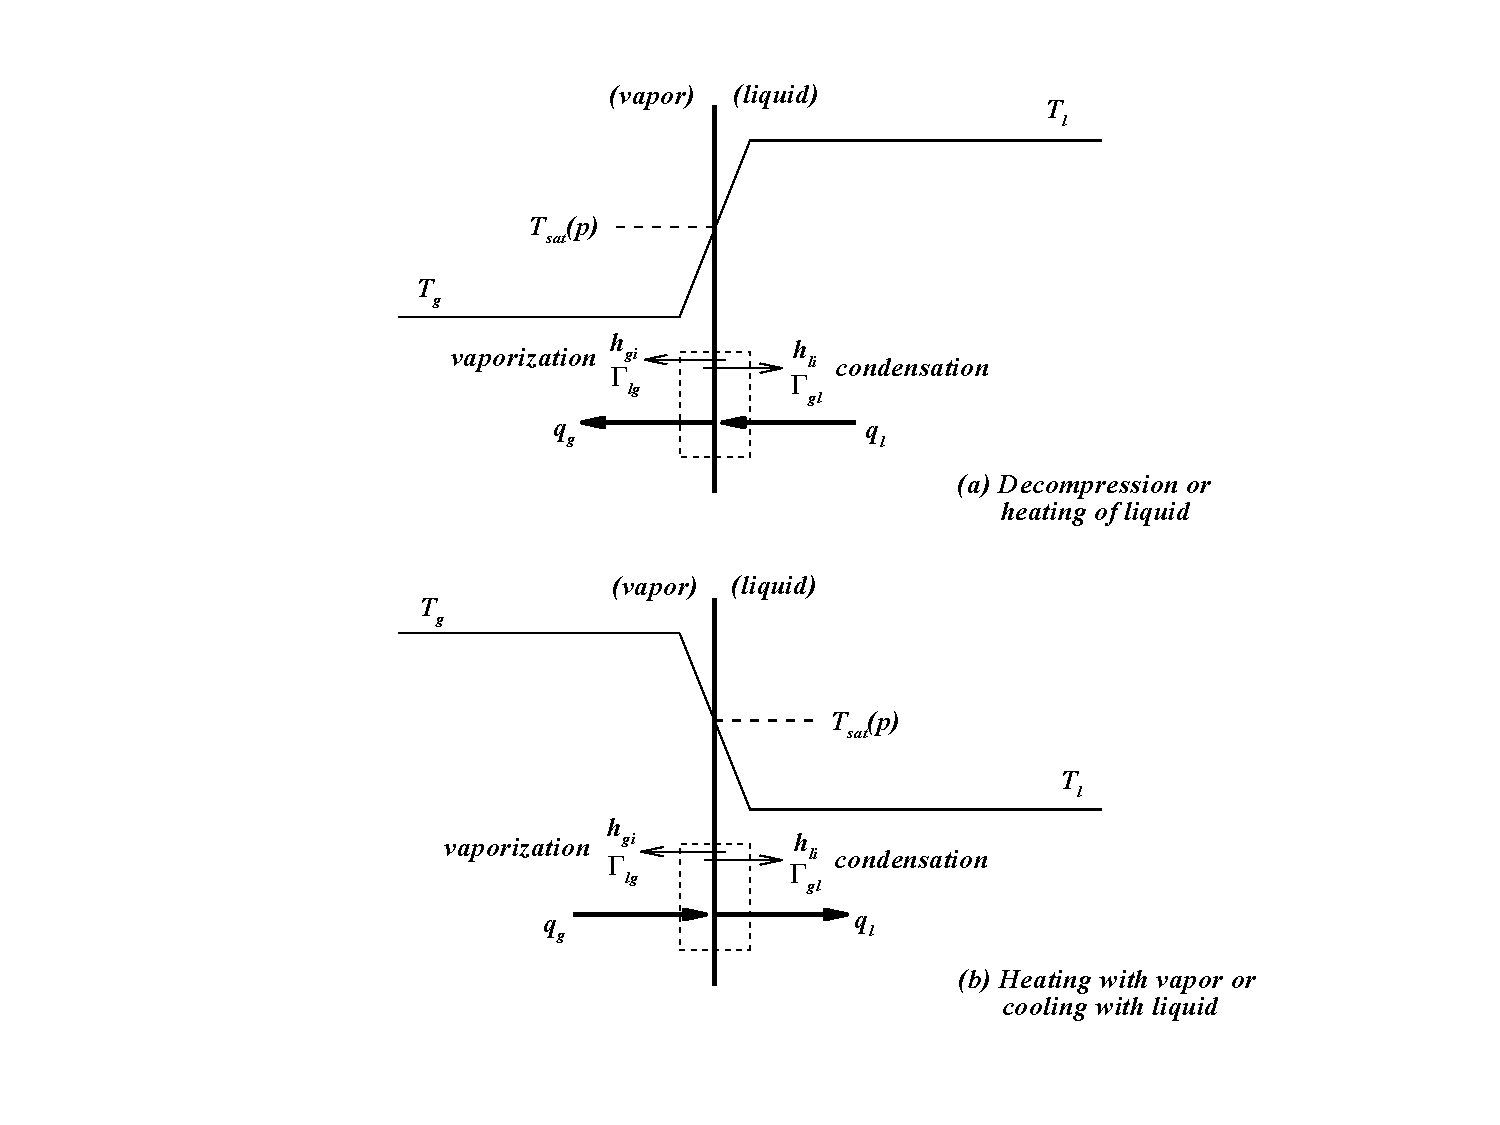
\includegraphics[clip=true,viewport=200 50 550 500,width=.8\textwidth]{figures/SEM/vaporization_condensation}
 %}
   \caption{Vaporization and condensation at a liquid-vapor interface
     (after Moody~\cite{Moody_1990}).\label{Berry-Fig:3}}
\end{figure}
Representative temperature profiles are shown for heat transfer from
vapor to liquid or liquid to vapor.  As discussed by
Moody~\cite{Moody_1990}, either vaporization or condensation can occur
for both temperature profiles. The interphase mass transfer is
determined by the net interfacial heat transfer: if net heat transfer
is toward the interface, vapor will form; conversely, if net heat
transfer is away from the interface, liquid will condense.
Figure~\ref{Berry-Fig:3} shows heat transfer rates $q_{vap}$ and
$q_{liq}$ from the vapor and liquid sides of the interface.  For
bidirectional phase change (vaporization and condensation), mass
transfer based on heat balance at the interface is adopted.  When
vaporization occurs, vapor is assumed to form at a saturated interface
temperature $T_{int}=T_{sat}(\bar{P}_{int})$.  If condensation occurs,
liquid is assumed to form also at a saturated interface temperature
$T_{int}=T_{sat}(\bar{P}_{int})$.  The interfacial total enthalpies $H_{k,int}$
correspond to the saturated values in order that the interphase mass
transfer rate and conservation of total energy be compatible:
\begin{equation}
  \label{E-R:95}
  H_{k,  int} = h_{k,  int} + \frac{1}{2} u_{int}^2
\end{equation}
for phase $k=(liq, vap)$, where $h_{k,int}$ is the phase $k$ specific enthalpy
evaluated at the interface condition.  Phasic specific enthalpy
depends upon the equation of state used and will be discussed with the
equations of state.  The interfacial density corresponds to the liquid
saturated density $\rho_{int} = \rho_{liq, sat}(P_{int})$.

%-----------------------------------------------------------------------------------------
\subsubsection{Interface direct heat transfer}
%-----------------------------------------------------------------------------------------
Without wall boiling, a simple model for the direct convective heat transfer $Q{ \text{wall}}$
from the wall to fluid phase $k$ will be the same as that of a single-phase
except the duct wall area over which this heat transfer can occur is weighted
by the wetted fraction of the phase.  That is,
\begin{equation}
  Q_{ \text{wall}, k } = h_{w,k} P_w \left(T_k  - T_{ \text{wall} } \right) \alpha_k
\end{equation}
for phase $k=(liq, vap)$, where $h_{w,k}$ is the convective wall heat transfer
coefficient associated with phase $k$ and $P_w$ is the wall-heated perimeter. Similarly, the direct heat
transfer from/to the interface to/from the phase $k$, which will also
be used to determine the mass transfer between the phases, is
\begin{equation}
  Q_{int,  k} = h_{T,  k}  \left( T_{int} - T_k \right)  A_{int}  A
\end{equation}
with $h_{T,  k}$ denoting the convective heat transfer coefficient
between the interface and phase $k$. The phasic bulk
temperature $T_k$ is determined from the respective phase's equation of
state.
%-----------------------------------------------------------------------------------------
\subsubsection{Stiffened Gas Equation of State (SGEOS) for two-phase flows} \label{sec:SGEOS}
%-----------------------------------------------------------------------------------------
With the seven-equation two-phase model each phase is compressible and
behaves with its own convex equation of state (EOS).  For initial
development purposes it was decided to use a simple form capable of
capturing the essential physics.  For this purpose the stiffened
gas equation of state (SGEOS)~\cite{SGEOS} was selected (as
it was also for single phase),
\begin{equation}
  \label{E-R:96}
  P_k(\rho_k,e_k) = (\gamma_k -1) \rho_k (e_k - q_k) - \gamma P_{k,\infty}
\end{equation}
where $P_k$, $\rho_k$, $e_k$, and $q_k$ are the pressure, density,
internal energy, and the binding energy of the fluid considered, respectively.  The
parameters $\gamma_k$, $q_k$, and $P_{k,\infty}$ are fluid-dependent coefficients. The first term on the right hand side
is a repulsive effect that is present for any state (gas, liquid, or
solid), and is due to molecular vibrations.  The second term on the
right represents the attractive molecular effect that guarantees the
cohesion of matter in the liquid or solid phases.  The parameters used
in this SGEOS are determined by using a reference curve, usually in
the $\left(P_k, \frac{1}{\rho_k}\right)$ plane.

To extend this equation of state for two phases,
LeMetayer~\cite{SGEOS} uses the saturation curves as this
reference curve to determine the stiffened gas parameters for liquid
and vapor phases.  The SGEOS is the simplest prototype that contains
the main physical properties of pure fluids, repulsive and attractive
molecular effects, thereby facilitating the handling of the essential
physics and thermodynamics with a simple analytical formulation.  Thus
each fluid has its own thermodynamics.  For each phase the
thermodynamic state is determined by the SGEOS:
\begin{align}
  \label{E-R:97}
  e_k(P_k,\rho_k) &= \frac{P_k+\gamma_k P_{k,\infty}}{(\gamma_k -1) \rho_k} + q_k
  \\
  \label{E-R:98}
  \rho_k (P_k,T_k) &= \frac{P_k+P_{k,\infty}}{(\gamma_k -1) c_{k,v} T_k}
  \\
  \label{E-R:99}
  h_k(T_k) &= \gamma_k  c_{k,v} T_k + q_k
  \\
  \label{E-R:100}
  g_k(P_k,T_k) &= \left(\gamma_k c_{k,v} - q^{'}_k \right) T_k - c_{k,v} T_k \ln \frac{T_k^\gamma}{\left(P_k+P_{k,\infty}\right)^{\gamma_k-1}} + q_k
\end{align}
where $T_k$, $h_k$, and $g_k$ are the temperature, enthalpy,
and Gibbs free enthalpy, respectively, of the phase considered.  In
addition to the three fluid parameters mentioned above, two
additional constants have been introduced, the constant
volume specific heat $c_{k,v}$ and the parameter $q^{'}_k$.  The method to
determine these parameters in liquid-vapor systems, and in particular
the coupling of liquid and vapor parameters, is given
in~\cite{SGEOS}.  The values for water and its vapor from that
reference are given in Table 2.  These parameter values appear to
yield reasonable approximations over a temperature range from 298K to
473K.  For higher temperature range the parameters can easily be
refit.

Unlike van der Waals type modeling where mass transfer is a
thermodynamic path, with the seven-equation two-phase model the mass
transfer modeling, which produces a relaxation toward thermodynamic
equilibrium, is achieved by a kinetic process.  Thus the seven-equation
model preserves hyperbolicity during mass transfer.
From equation~\eqref{E-R:99} it is readily seen that the phase
$k$ specific enthalpy evaluated at the interface condition from
equation~\eqref{E-R:95} is
\begin{equation}
  h_{k,  int} = c_{p, k}  T_{int} + q_k
\end{equation}
because $c_{p, k} = \gamma_k  c_{v, k}$.

The bulk interphase mass transfer from the liquid phase to the vapor
phase $\Gamma$ is due to their difference in Gibb's free energy.  At
saturated conditions the Gibb's energies of the two phases are equal.
It is necessary to determine the saturation temperature $T_{sat}(P)$
for given pressure $P=\bar{P}_{int}$ and the heat of vaporization
$L_v\left(T_{sat}(\bar{P}_{int}) \right)$ at this saturation temperature
with the SGEOS for each phase.  For this calculation, the procedure
of~\cite{SGEOS} is adopted.  This procedure for the
determination of SGEOS parameters can be made very accurate provided
the two reference states are chosen sufficiently close to represent
the experimental saturation curves as locally quasi-linear.
Restrictions occur near the critical point, but away from this point,
a wide range of temperatures and pressures can be considered.  At
thermodynamic equilibrium at the interface, the two phasic Gibbs free
enthalpies must be equal, $g_{vap}=g_{liq}$, so the use of equation~\eqref{E-R:100}
yields
\begin{equation}
  \label{E-R:102}
  \ln \left( P + P_{\infty,  vap} \right) = A + \frac{B}{T} + C  \ln(T) + D  \ln \left( P + P_{\infty,  liq} \right)
\end{equation}
where
\begin{align}
  A &= \frac{c_{p, liq} - c_{p, vap} + q'_{vap} - q'_{liq}}{c_{p,  vap} - c_{v,  vap}} \\
  B &= \frac{q_{liq}-q_{vap}}{c_{p,  vap} - c_{v,  vap}} \\
  C &= \frac{c_{p, vap} - c_{p, liq}}{c_{p,  vap} - c_{v,  vap}} \\
  D &= \frac{c_{p, liq} - c_{v, liq}}{c_{p,  vap} - c_{v,  vap}} \,\,.
\end{align}
Relation~\eqref{E-R:102} is nonlinear, but can used to compute the
theoretical curve $T_{sat}(P)$.  A simple Newton iterative numerical
procedure is used.  With $T_{sat}(P)$ determined, the heat of
vaporization is calculated as
\begin{align}
  \nonumber
  L_v \left( T_{int} \right) &= h_{vap,  int} - h_{liq,  int}
  \\
  \nonumber
  &= h_{k,  int}
  \\
  &= \left( \gamma_{vap}  c_{v, vap}  T + q_{vap} \right) - \left( \gamma_{liq}  c_{v, liq}  T + q_{liq} \right) \,.
\end{align}
%
%===================================================================================
\section{A viscous regularization for the multi-D seven-equation model}\label{sec:sev-equ-visc-reg-sect4}
%===================================================================================
In this section, the dissipative terms for the multi-D seven-equation model \emph{with pressure and velocity relaxation source terms} are derived (the mass and energy transfer terms are omitted). The methodology proposed in  \chap{chap:theory_chp1} is followed. For clarity purpose, the seven-equation model with pressure and velocity relaxation terms is recalled when considering a phase $k$ in interaction with a second phase $j$:
%
\begin{subequations}\label{eq:sev_equ}
\begin{align}
\partial_t \left( \alpha_k  A\right) + A \mbold u_{int} \cdot \grad \alpha_k = A \mu_P \left( P_k - P_j \right)
\end{align}
\begin{align}
\partial_t \left( \alpha_k \rho_k A \right) + \div \left( \alpha_k \rho_k \mbold u_k A \right) = 0
\end{align}
\begin{align}
\partial_t \left( \alpha_k \rho_k u_k A \right) + \div \left[ \alpha_k A \left( \rho_k \mbold u_k \otimes \mbold u_k + P_k \mathbb{I} \right) \right] &=\nonumber\\
\alpha_k P_k \grad A + P_{int} A \grad \alpha_k &+ A \lambda_u \left( \mbold u_j - \mbold u_k \right)
\end{align}
\begin{align}
\partial_t \left( \alpha_k \rho_k E_k A \right) + \div \left[ \alpha_k A \mbold u_k \left( \rho_k E_k + P_k \right) \right] &=\nonumber\\
A P_{int} \mbold u_{int} \cdot \grad \alpha_k - \mu_P \bar{P}_{int} \left( P_k-P_j \right) &+ A \lambda_u \bar{\mbold u}_{int} \cdot \left( \mbold u_j - \mbold u_k \right)
\end{align}
\end{subequations}
%
%where $\rho_k$, $u_k$, $E_k$ and $P_k$ are the density, the velocity, the specific total energy and the pressure of $k^{th}$ phase, respectively. The pressure and velocity relaxation parameters are denoted by $\mu$ and $\lambda$, respectively. The variables with index $_I$ correspond to the interfacial variables and a definition for those can be found in \cite{SEM}. The cross-section $A$ is only function of space: $\partial_t A = 0$.
In order to apply the EVM, dissipative terms are added to each equation of the system given in \eqt{eq:sev_equ}, which yields:
%
\begin{subequations}\label{eq:sev_equ-with-diss-terms}
\begin{align}\label{eq:sev_equ-with-diss-terms-vf}
\partial_t \left( \alpha_k  A\right) + \mbold u_{int} A \grad \alpha_k = A \mu_P \left( P_k - P_j \right) + \div \mbold l_k
\end{align}
\begin{align}\label{eq:sev_equ-with-diss-terms-cont}
\partial_t \left( \alpha_k \rho_k A \right) + \div \left( \alpha_k \rho_k \mbold u_k A \right) = \div \mbold f_k
\end{align}
\begin{align}\label{eq:sev_equ-with-diss-terms-mom}
\partial_t \left( \alpha_k \rho_k \mbold u_k A \right) + \div \left[ \alpha_k A \left( \rho_k \mbold u_k \otimes \mbold u_k + P_k \mathbb{I} \right) \right] &=\nonumber\\
\alpha_k P_k \grad A + P_{int} A \grad \alpha_k &+ A \lambda_u \left( \mbold u_j - \mbold u_k \right) + \div \mbold g_k
\end{align}
\begin{align}\label{eq:sev_equ-with-diss-terms-ener}
\partial_t \left( \alpha_k \rho_k E_k A \right) + \div \left[ \alpha_k A \mbold u_k \left( \rho_k E_k + P_k \right) \right] &=\nonumber\\
P_{int} A \mbold u_{int} \cdot \grad \alpha_k - \mu_P \bar{P}_{int} \left( P_k-P_j \right) &+ A \lambda_u \bar{\mbold u}_{int} \cdot \left( \mbold u_j - \mbold u_k \right) + \div \left( \mbold h_k + \mbold u \cdot \mbold g_k \right)
\end{align}
\end{subequations}
%
where $\mbold f_k$, $\mbold g_k$, $\mbold h_k$ and $\mbold l_k$ are the dissipative terms. The next step consists of deriving the entropy equation for the phase $k$, on the same model as what is done in \app{app:sev-equ-model-entropy}. Extra terms will appear in the right-hand-side of the entropy equation due to the dissipative terms. By choosing properly the definition of the dissipative terms, the sign of these extra terms can be controlled in order to ensure positivity of the entropy residual:
%
\begin{enumerate}
\item recast the system of equation given in \eqt{eq:sev_equ-with-diss-terms} in terms of the primitive variables $(\alpha_k, \rho_k, \mbold u_k, e_k)$.
\item derive the entropy equation by using the chain rule:
\begin{equation}
\label{eq:chain_rule-sct4}
\frac{Ds_k}{Dt} = \left( s_{\rho} \right)_k \frac{D \rho_k}{Dt} + \left( s_{e} \right)_k \frac{D e_k}{Dt} 
\end{equation}
where $\frac{D \cdot}{Dt}$ is the material derivative. The terms $(s_e)_k$ and $(s_{\rho})_k$ denote the partial derivative of the entropy $s_k$ with respect to $e_k$ and $\rho_k$, respectively.
\item isolate the terms of interest and choose an appropriate expression for each of the dissipative terms in order to ensure positivity of the right-hand side.
\end{enumerate}
%
We first recast \eqt{eq:sev_equ-with-diss-terms} in terms of the primitive variables: the volume fraction equation remains unchanged. The equation for the primitive variable $\rho_k$ is derived by combining \eqt{eq:sev_equ-with-diss-terms-vf} and \eqt{eq:sev_equ-with-diss-terms-cont}:
%
\begin{equation}\label{eq:rho-7-eqn-model-sect4}
\alpha_k A \left[ \partial_t \rho_k + \left( \mbold u_k - \textcolor{blue}{\mbold u_{int}} \right) \cdot \grad \rho_k \right] = \textcolor{blue}{A \rho_k \mu_P \left( P_k - P_j \right)} + \div \mbold f_k - \rho_k \div \mbold l_k
\end{equation}
%
The velocity equation is obtained by subtracting the density equation from the momentum equation:
%
\begin{align}\label{eq:vel-7-eqn-model-sect4}
\alpha_k \rho_k  A \left[ \partial_t \mbold u_k + \mbold u_k \cdot \div \mbold u_k \right]  + \div \left( \alpha_k \rho_k A P_k \mathbb{I} \right) &=\nonumber\\
\textcolor{blue}{\alpha_k P_k \grad A + P_{int} A \grad \alpha_k + A \lambda \left( \mbold u_j - \mbold u_k \right)} &+ \div \mbold g_k - \mbold u_k \otimes \mbold f_k
\end{align}
%
After multiplying \eqt{eq:vel-7-eqn-model-sect4} by the velocity vector $\mbold u_k$, the resulting kinetic energy equation is subtracted from the total energy equation to obtain the internal energy equation for phase $k$:
%
\begin{align}\label{eq:int-ener-7-eqn-model-sect4}
\alpha_k \rho_k  A \left[ \partial_t \mbold e_k + \mbold u_k \cdot \div \mbold e_k \right]  + \alpha_k \rho_k A P_k \grad \mbold u_k &=\nonumber\\
\textcolor{blue}{P_{int} A \left(\mbold u_{int}-\mbold u_k \right) \cdot \grad \alpha_k} &-  \textcolor{blue}{\alpha_k P_k \mbold u_k \grad A} \nonumber \\ 
\textcolor{blue}{-\bar{P}_{int} A \mu_P \left(P_k-P_j \right)} &+ \textcolor{blue}{A \lambda_u \left(\mbold u_j-\mbold u_k  \right) \cdot \left(\bar{\mbold u}_{int}- \mbold u_k \right)}\nonumber \\
&+ \div \mbold h_k + \mbold g_k : \grad \mbold u_k + || \mbold u ||^2_k \mbold f_k
\end{align}
%
The blue terms in \eqt{eq:rho-7-eqn-model-sect4} and \eqt{eq:int-ener-7-eqn-model-sect4} yield the positive terms in the right-hand-side of \eqt{eq:ent-eqn-7-eqn-model} and thus are ignored in the remaining of the derivation. The entropy equation is now obtained by combining the density equation (\eqt{eq:rho-7-eqn-model-sect4}) and the internal energy equation (\eqt{eq:int-ener-7-eqn-model-sect4}) through the chain rule given in \eqt{eq:chain_rule-sct4} to yield:
%
\begin{equation}\label{eq:ent-res-7-eqn-diss-terms}
\alpha_k \rho_k A \frac{Ds_k}{Dt} = \left(s_e\right)_k \left[ \div \mbold h_k + \mbold g_k : \grad \mbold u_k +  \left( || \mbold u ||^2_k - e_k\right) \div \mbold f_k  \right] + (\rho s_\rho)_k \left[ \div \mbold f_k - \rho_k \div \mbold l_k \right].
\end{equation}
%
where it was assumed that the entropy of phase $k$ satisfies the second thermodynamic law: 
%
\begin{align}\label{eq:2nd-therm-laws-sect4}
&T_k \text{d} s_k = \text{d}e_k - P_k\frac{\text{d}\rho_k}{\rho_k^2} \nonumber \\
& \text{which implies } P_k (s_e)_k + \rho_k (s_\rho)_k = 0, \\
& (s_e)_k = T_k^{-1} \text{ and } (s_\rho)_k = - (s_e)_k P_k \frac{\text{d}\rho_k}{\rho_k^2}. \nonumber
\end{align}
% 
From this point, two options are available in order to derive the dissipative terms: either we consider the total entropy residual of the system by summing \eqt{eq:ent-res-7-eqn-diss-terms} over each phase, or we can consider each phase independently. This dilemma can be answered by remembering that the seven-equation model degenerates into the single phase flow equations in the limits $\alpha_k = 0,1$. Thus, the dissipative terms also have to be consistent with the single-phase flow limits. As a result, it is chosen to derive the dissipative terms by considering each phase independently which will automatically ensure positivity of the total entropy residual as well.

The right-hand side of \eqt{eq:ent-res-7-eqn-diss-terms} can be further simplified by using the following expression
for the dissipative terms $\mbold f_k$,  $\mbold g_k$ and $\mbold h_k$:
\begin{align}\label{eq:def-diss-terms-sect4}
  \mbold f_k &= \tilde{\mbold f}_k + \rho_k \mbold  l_k 
  \\
  \mbold g_k &= \alpha_k \rho_k A \mu_k \mathbb{F}(\mbold u_k) + \mbold f_k \otimes \mbold u_k
  \\
  \mbold h_k &= \tilde{\mbold h}_k - \frac{|| \mbold u||^2 }{2} \mbold f_k + (\rho e)_k \mbold l_k.
\end{align}
Note the area function $A$ in the definition of $\mbold g$. It yields:
%
\begin{align}\label{eq:ent-res-7-eqn-diss-terms2}
&\alpha_k \rho_k A \frac{Ds_k}{Dt} = \nonumber \\
&\underbrace{\left(s_e\right)_k \alpha_k \rho_k A \mu_k \mathbb{F}(\mbold u_k) : \grad \mbold u_k}_{\mathcal{R}_1} +
\underbrace{\left[ \div \tilde{\mbold h}_k  - e_k \div \tilde{\mbold f}_k  \right] + (\rho s_\rho)_k \div \tilde{\mbold f}_k}_{\mathcal{R}_2} + \nonumber \\
&\underbrace{(s_e)_k \div \left( \rho_k e_k \mbold l_k \right) -  (s_e)_k e_k \div \left( \rho_k \mbold l_k \right) + \rho_k (s_\rho)_k \div \left( \rho_k \mbold l_k \right) 
  - \rho_k^2 (s_\rho)_k \div \mbold l_k}_{\mathcal{R}_3},
\end{align}
%
where $\mu_k$ is a positive viscosity coefficient for phase $k$. For simplicity, the right-hand-side of \eqt{eq:ent-res-7-eqn-diss-terms2} is split into three terms denoted by $\mathcal{R}_1$, $\mathcal{R}_2$ and $\mathcal{R}_3$. Since $(s_e)_k$ is defined as the inverse of the temperature and thus positive, the sign of the first term, $\mathcal{R}_1$, is conditioned by the choice of the function $\mathbb{F}(\mbold u_k)$ so that the product with the tensor $\grad \mbold u_k$ is positive. As in \cite{jlg}, $\mathbb{F}(\mbold u_k)$ is chosen proportional to the symmetric gradient of the velocity vector $\grad^s \mbold u_k$, whom entries are given by $(\grad^s \mbold u)_{i,j} = \frac{1}{2} \left( \partial_{x_i} u_i + \partial_{x_j} u_j \right)$. Such a choice ensures the associated dissipative terms to be rotationally invariant and also positivity of $\mathcal{R}_1$. An other option would be to simply set $\mathbb{F}(\mbold u_k)$ proportional to $\grad \mbold u_k$ which allows to recover the parabolic regularization. 

After a few lines of algebra, the third term ${\mathcal{R}_3}$ can be recast as a function of the gradient of the entropy as follows:
\begin{align}
 \label{eq:ent-R3-sct4}
  \mathcal{R}_2  =  \rho_k A \mbold l_k \cdot \grad s_k.
\end{align} 
One of the assumptions made in the entropy minimum principle is to that the entropy 
is at a minimum which implies that its gradient is null. Because of this, it follows that
the term $\mathcal{R}_3$ is zero at the minimum and thus, the entropy minimum principle is verified
independently of the definition of the dissipative term $\mbold l_k$ used in the volume fraction
equation. It will be explained later in this section how to derive a definition for $\mbold l_k$.

We now focus on the term denoted by $\mathcal{R}_2$, that is found identical to the right-hand-side of the single phase entropy equation obtained from the multi-D Euler equations (see \eqt{eq:rhs-euler-equ-app1} in \app{app:diss_terms}). Thus, following \cite{jlg} and also \app{app:diss_terms}, the term $\mathcal{R}_2$ is known to be positive when (i) assuming concavity of the entropy function $s_k$ with respect to the internal energy $e_k$ and the specific volume $1 / \rho_k$ (or convexity of $-s_k$) and (ii) choosing the following definitions for the dissipative terms $\tilde{h}_k$ and $\tilde{f}_k$:
%
\begin{align}
&\tilde{\mbold f}_k = \alpha_k A \kappa_k \grad \rho_k \\
&\tilde{\mbold h}_k = \alpha_k A \kappa_k \grad \left( \rho e \right)_k,
\end{align}
%  
where $\kappa_k$ is another positive viscosity coefficient. The entropy equation can now be written in its final form:
%
\begin{align}\label{eq:ent-res-7-eqn-diss-terms3}
&\alpha_k \rho_k A \frac{Ds_k}{Dt} - \mbold f_k \cdot \grad s_k - \div \left( \alpha_k \rho_k A \grad s_k \right) = \nonumber\\
&- \alpha_k A \kappa_k \mathbf{Q}_k + (s_e)_k \alpha_k A \rho_k \mu_k \grad^s \mbold u_k : \grad \mbold u_k,
\end{align}
%
where $\mathbf{Q}_k$ is a negative semi-definite quadratic form defined as:
%
\begin{eqnarray}
\mathbf{Q}_k &=& X^t_k \Sigma_k X_k \nonumber \\
\text{with } X_k &=& \begin{bmatrix}
\grad \rho_k \\
\grad e_k 
\end{bmatrix}
\text{and } \Sigma_k = \begin{bmatrix}
       \partial_{\rho_k} (\rho^2_k \partial_{\rho_k} s_k) & \partial_{\rho_k,e_k} s_k  \\[0.3em]
       \partial_{\rho_k,e_k} s_k & \partial_{e_k,e_k} s_k           \\[0.3em]
     \end{bmatrix}. \nonumber 
\end{eqnarray}
%
\eqt{eq:ent-res-7-eqn-diss-terms3} is used to prove the entropy minimum principle: assuming that $s_k$ reaches its minimum value in $\mbold r_{min}(t)$ at each time $t$, the gradient, $\grad s_k$, and Laplacian, $\Delta s_k$,  of the entropy are null and positive at this particular point, respectively. Furthermore, it is recalled that the viscosity coefficients $\mu_k$ and $\kappa_k$ are positive by definition. Then, because the right-hand-side of \eqt{eq:ent-res-7-eqn-diss-terms3} is proven positive, the entropy minimum principle holds for each phase $k$, \textbf{independently of the definition of the dissipative term} $\mbold l_k$, such as:
%
\begin{equation}\label{eq:ent-res-7-eqn-diss-terms4}
\alpha_k \rho_k A \partial_t s_k(\mbold r_{min},t)) \geq 0 \Rightarrow \partial_t s_k(\mbold r_{min},t)) \geq 0 \nonumber
\end{equation}
%

It remains to obtain a definition for the
dissipative term $\mbold l_k$ used in the volume fraction equation. A way to achieve this is to
consider the volume fraction equation, \eqt{eq:sev_equ-with-diss-terms-vf}, by itself and notice that it is an hyperbolic equation
with eigenvalue $\mbold u_{int}$. An entropy equation can be derived and used to prove the
entropy minimum principle by properly choosing the dissipative term. The objective is to
ensure positivity of the volume fraction and also uniqueness of the weak solution. Following
the work of Guermond et al. in \cite{jlg1, jlg2} and by analogy
with Burger's equation described in \chap{chap:burger_chap3}, it can be shown that a dissipative term ensuring positivity and
uniqueness of the weak solution for the volume fraction equation, is of the form $\mbold l_k = \beta_k A \grad \alpha_k $ where $\beta_k$
is a positive viscosity coefficient.

All of the dissipative terms are now defined and recalled here:
%
\begin{subequations}\label{eq:visc-reg-7-equ-sect4}
\begin{align}
  \mbold l_k &= \beta_k A \grad \alpha_k 
\end{align}
\begin{align}
  \mbold f_k &= \alpha_k A \kappa_k \grad \rho_k + \rho_k A \mbold l_k 
\end{align}
\begin{align}
  \mbold g_k &= \alpha_k A \mu_k \rho \grad^s \mbold u_k 
\end{align}
\begin{align}
  \mbold h_k &=  \alpha_k A \kappa_k \grad \left( \rho e \right)_k + \mbold u_k : \mbold g_k - \frac{|| \mbold u_k||^2}{2} \mbold f_k + (\rho e)_k \mbold l_k 
\end{align}
\end{subequations}
%
At this point, some remarks are in order:
\begin{enumerate}
\item {The viscous regularization given in \eqt{eq:visc-reg-7-equ-sect4} for the multi-D seven-equation model, is equivalent to the parabolic regularization \cite{Parabolic} when assuming $\beta_k = \kappa_k$ and $\mathbb{F}(\mbold u_k) = \alpha_k \rho_k \kappa_k \grad \mbold u_k$. However, decoupling between the regularization on the velocity and on the density in the momentum equation is important to make the regularization rotation invariant but also to ensure well-scaled dissipative terms for a wide range of Mach number as was shown in \chap{chap:euler} for the multi-D Euler equations.}
\item {The dissipative term $\mbold l_k$ requires the definition of a new viscosity
    coefficient $\beta_k$. It was shown that this viscosity coefficient is independent of
    the other viscosity coefficients $\mu_k$ and $\kappa_k$. Its definition should
    account for the eigenvalue associated with the void fraction equation $\mbold u_{int}$.
    In addition, an entropy residual can be determined by analogy to Burger's
    equation. }
%    It is noted, however, that the eigenvalue $\mbold u_{int}$ can be discontinuous
%    since its definition involves the sign of the void fraction gradient, which
%    makes the theory more challenging. For simplicity, we ignore this aspect of the
%    theory in this report.\tcr{maybe for a report, but here you should say a bit more}}

\item {The dissipative term $\mbold f_k$ is a function of $\mbold l_k$. Thus, all of the other
    dissipative terms are also functions of $\mbold l_k$.}

\item {The partial derivatives $(s_e)_k$ and $(s_{\rho_k})_k$ can be computed using the
    definition provided in \eqt{eq:2nd-therm-laws-sect4} and are functions of the thermodynamic
    variables: pressure, temperature and density.}

\item {All of the dissipative terms are chosen to be proportional to the the void
    fraction $\alpha_k$ and the cross-sectional area $A$, but the one in the volume fraction equation that is only proportional to $A$. For instance, $\alpha_k A \grad \rho_k$ is the
    flux of the dissipative term in the continuity equation through the area seen
    by the phase $\alpha_k A$. When one of the phases disappears, the dissipative terms
    must to go to zero for consistency. On the other hand, when $\alpha_k$ goes to one,
    the single-phase equation must be recovered. }
    
\item{Compatibility of the viscous regularization proposed in \eqt{eq:visc-reg-7-equ-sect4} with the generalized entropies identified in Harten et al. \cite{Harten} has not been investigated yet. However, it is believed that the entropy inequalities still holds because of the similarities of the entropy residual for the multi-D seven-equation model with the entropy residual derived in the single phase flow case \cite{jlg}.} 
%A rigorous proof is ongoing work and will be included in the final version.
%\tcr{don't you want to include this in the final version?} \tcb{I do}}
\end{enumerate}
%
Through the derivations of the viscous regularization, it was noted that another set of dissipative terms $\mbold f_k$ and $\mbold l_k$ would also ensures positivity of the entropy residual:
%
\begin{subequations}
\begin{align}\label{eq:def-l-k-wrong-sect4}
\mbold l_k =\beta_k T_k \left[ \frac{\rho_k}{P_k+\rho_k e_k} \grad \left( \frac{P_k}{\rho_k e_k} \right) - \frac{1}{P_k} \grad \rho_k \right]
\end{align}
\begin{align}
\mbold f_k = \kappa_k \grad \rho_k +  \frac{\rho^2_k (s_{\rho})_k}{\left( \rho s_{\rho} - e s_e \right)_k} \mbold l_k
\end{align}
\end{subequations}
%
However, the definition of $\mbold l_k$ proposed in \eqt{eq:def-l-k-wrong-sect4} was not considered as valid for the following reasons: positivity of the volume fraction cannot be achieved and the parabolic regularization is not retrieved.

A rotation invariant viscous regularization for the multi-D seven-equation model is now available involving three viscosity coefficients $\beta_k$, $\mu_k$ and $\kappa_k$, for each phase $k$. Definition of these viscosity coefficients is the purpose of the next section (\sect{sec:sev-equ-visc-coeff-sect4}).
%===================================================================================
\section{Low-mach asymptotic limit and viscosity coefficients}\label{sec:sev-equ-visc-coeff-sect4}
%===================================================================================
This section aims at deriving a definition of the viscosity coefficients involved in the viscous regularization for the multi-D seven-equation model. We propose to follow the same methodology as in \chap{chap:euler} for the multi-D Euler equations: after obtaining the non-dimensional equations, a definition for the viscosity coefficients is derived based on the entropy residual and consistent with the low-Mach asymptotic limit. Particular attention is paid to the definition of the viscosity coefficient $\beta_k$ used in the volume fraction equation.

Using the EVM to define the viscosity coefficients is not the unique option here. Other numerical methods initially developed for single-phase flows, such as pressure-based and Lapidus viscosity methods, could be used as a starting point and adapted to the seven-equation model. Such a reasoning is motivated by one of the initial assumptions of the seven-equation model that assumes each phase verifies the Euler equations.
%------------------------------------------------------------------------------------------------------
\subsection{Definition of the viscosity coefficients}\label{sec:visc-coeff-sem}
%------------------------------------------------------------------------------------------------------
The viscous regularization derived in \sect{sec:sev-equ-visc-reg-sect4} for the multi-D SEM requires three viscosity coefficients for each phase $k$ denoted by $\beta_k$, $\mu_k$ and $\kappa_k$. Following the methodology detailed in \sect{sec:hyp_sect1b}, for each viscosity coefficient an upper bound, denoted by the subscript $max$, is defined and referred to as the first-order viscosity coefficient, along with a entropy viscosity coefficient that is set proportional to an entropy residual and denoted by the subscript $e$:
%
\begin{align}\label{eq:def-visc-sem-sct4}
\beta_k( \mbold r, t) = \min \left( \beta_{e,k}( \mbold r, t), \beta_{max,k} ( \mbold r, t) \right), \nonumber \\
\mu_k( \mbold r, t) = \min \left( \mu_{e,k}( \mbold r, t), \mu_{max,k} ( \mbold r, t) \right), \nonumber \\
\kappa_k( \mbold r, t) = \min \left( \kappa_{e,k}( \mbold r, t), \kappa_{max,k} ( \mbold r, t) \right) \,. \nonumber
\end{align}
% 
where all of the variables are locally defined. As for the multi-D single-phase Euler equations and for the same reasons, the entropy residual for each phase $k$ is recast as a function of the pressure, the velocity, the density and the speed of sound as follows:
%
\begin{equation}\label{eq:ent_res-sem-sct4}
\resi_k(\mbold r,t) := \partial_t s_k + \mbold u_k \cdot \grad s_k = \matder{s_k} = \frac{(s_e)_k}{(P_e)_k} \left( \underbrace{\matder{P_k} - c_k^2 \matder{\rho_k} }_{\resinew_k(\mbold r,t)} \right) ,
\end{equation} 
%
where $\resinew_k(\mbold r,t)$ is the new entropy residual of phase $k$ and will experience the same variations as $\resi_k(\mbold r,t)$. 

We first choose to investigate the definitions of the high and first-order viscosity coefficients for $\mu_k$ and $\kappa_k$. It is noted that the dissipative terms function of $\mu_k$ and $\kappa_k$ are the same as the ones for the single-phase Euler equation when considering $\tilde{A} = \alpha_k A$ as a pseudo cross section. Furthermore, we need to ensure consistency with the single-phase Euler equation in the limits $\alpha_k \to 1$. Thus, based on the work done in \sect{sec:new_ent_prod} , the first order viscosity coefficients are set proportional to the local maximum eigenvalue $\lambda_k$,
%
\begin{equation}\label{eq:def-visc-max-sem-sct4}
\kappa_{max,k}( \mbold r, t) = \mu_{max,k}( \mbold r, t) = \frac{h}{2} \left( || \mbold u_k|| + c_k \right)
\end{equation}
%
and the entropy viscosity viscosity coefficients are defined as
%
\begin{subequations}
\label{eq:visc_definition-sct4}
\begin{equation}
\mu_{e,k}(\mbold r,t)    = h^2 \frac{\max\left( | \resinew_k(\mbold r_q,t) |\,, || \mbold u_k(\mbold r_q,t) || J[P_k](t) \,, || \mbold u_k(\mbold r_q,t) || c_k^2(\mbold r_q,t) J[\rho_k](t) \right)}{\norm_{P,k}^\mu}    \, ,
\end{equation} 
\text{and} 
\begin{equation}
\kappa_{e,k}(\mbold r,t) = h^2 \frac{\max\left( | \resinew_k(\mbold r_q,t) |\,, || \mbold u_k(\mbold r_q,t) || J[P_k](t) \,, || \mbold u_k(\mbold r_q,t) || c_k^2(\mbold r_q,t) J[\rho_k](t) \right)}{\norm_{P,k}^\kappa} \, .
\end{equation}
\end{subequations}
%
where $h$ is the grid size and $J[x](t)$ denotes the jump of the quantity $x$ and was defined in \chap{chap:disc_chap2}. The normalization parameters $\norm_{P,k}^\mu$ and $\norm_{P,k}^\kappa$ will be determined later in this section by inspecting the non-dimensional version of the seven-equation model.

It remains to specify the viscosity coefficients $\beta_e$ and $\beta_{max}$. For the purpose of this paragraph, let us consider the scalar volume fraction equation and assume that the interface velocity $\mbold u_{int}$ is given. Because it is a scalar hyperbolic equation, it is proposed to define the high and first-order viscosity coefficients on the same model as Burger's equation. Thus, $\beta_{max}$ is set proportional to the eigenvalue that is the interface velocity $\mbold u_{int}$,
%
\begin{equation}\label{eq:def-beta-max-sen-sect4}
\beta_{max,k}( \mbold r, t) = \frac{h}{2} || \mbold u_{int} ||,
\end{equation}
%
whereas the entropy viscosity viscosity coefficient $\beta_e$ is function of an entropy residual, $R_{\alpha,k}$, derived from the volume fraction equation for phase $k$ as follows:
%
\begin{align}\label{eq:def-beta-sen-sect4}
\beta_{e,k}( \mbold r, t) = h^2 \frac{\max\left( | R_{\alpha,k}(\mbold r_q,t) |\,, || \mbold u_{int}(\mbold r_q,t) || J[\alpha_k](t) \right)}{\norm_{k}^\beta} \,
\end{align}
%
where $\norm_{k}^\beta$ denotes a normalization parameters whom definition will be further investigated. To derive the entropy residual $R_{\alpha,k}$, we consider the volume fraction equation for phase $k$ with its viscous regularization and assume the existence of a mathematical entropy denoted by $\eta(\alpha_k)$:
%
\begin{equation}\label{eq:vf-sem-sct4}
\partial_t \left(A \alpha_k \right) + A \mbold u_{int} \cdot \grad \alpha_k = \div \left( \beta_k A \grad \alpha_k \right)
\end{equation}
% 
After multiplying by $\frac{\text{d} \eta (\alpha_k)}{\text{d} \alpha_k}$ and using the chain rule, an expression for the entropy residual $R_{\alpha,k}$ is obtained:
%
\begin{equation}\label{eq:vf-sem2-sct4}
R_{\alpha,k} = \partial_t \left(A \eta(\alpha_k) \right) + A \mbold u_{int} \cdot \grad \eta(\alpha_k) = \frac{\text{d} \eta (\alpha_k)}{\text{d} \alpha_k} \div \left( \beta_k A \grad \alpha_k \right)
\end{equation}
% 
Because \eqt{eq:vf-sem2-sct4} is identical to \eqt{eq:weak_sol8_sct1b}, it is concluded that $R_{\alpha,k} \geq 0$ when assuming $\eta$ convex with respect to $\alpha_k$, which justifies the definition of the entropy viscosity viscosity coefficient $\beta_{e,k}$ given in \eqt{eq:def-beta-sen-sect4} based on \eqt{sec:evm_hyp_sc_sct1b}. The entropy function is taken equal to $\eta(\alpha_k) = \frac{\alpha_k^2}{2}$ which is convex.
%------------------------------------------------------------------------------------------------------
\subsection{Low-mach asymptotic limit of the seven-equation model}\label{sec:low-Mach-sem}
%------------------------------------------------------------------------------------------------------
In order to have a complete definition for the viscosity coefficients $\beta_k$, $\mu_k$ and $\kappa_k$, the normalization parameters introduced in the definition of the entropy viscosity coefficients $\beta_{e,k}$, $\mu_{e,k}$ and $\kappa_{e,k}$ have to be determined. In \chap{chap:euler}, the normalization parameters were derived from the non-dimensionalized multi-D Euler equations in order to obtain well-scaled dissipative terms. Thus, it is proposed to follow the same method to derive the three normalization parameters $\norm_{P,k}^\mu$, $\norm_{P,k}^\kappa$ and $\norm_{k}^\beta$ used in the definition of the viscosity coefficients involved in the viscous regularization of the seven-equation model. For simplicity, the Ideal Gas equation of state is considered through the derivations.

For now, the definition of the viscosity coefficients is simply derived by analogy to \sect{sec:lowMach}. First, we define the far-field or stagnation coefficients for each phase as it is done in \eqt{eq:norm_param} by adding the subscript $k$ to $\infty$. Then, the scaled equations are derived for each phase which leads to the definition of a phasic P\'eclet and Reynolds numbers referred to as $\Pe_k$ and $\Re_k$, respectively, that are tied to the far-field or stagnation quantities of the viscosity coefficients $\mu_{k,\infty}$ and $\kappa_{k,\infty}$ as shown in \eqt{eq:ref_numb_7eq}:
%  
\begin{equation}
\label{eq:ref_numb_7eq}
\Re_{k,\infty} = \frac{u_{k,\infty} L_\infty}{\mu_{k,\infty}} \text{ and }
\Pe_{k,\infty} = \frac{u_{k,\infty} L_\infty}{\kappa_{k,\infty}} \, .
\end{equation}
%
Because the viscous regularization derived previously in \sect{sec:sev-equ-visc-reg-sect4} requires an extra viscosity coefficient $\beta_k$ for the volume fraction equation, a new P\'eclet number, $\Pe_{k,\infty}^\beta$ is also defined as follows,
%
\begin{equation}
\label{eq:ref_numb_7eq_beta}
\Pe_{k,\infty}^\beta = \frac{u_{int,\infty} L_\infty}{\beta_{k,\infty}} \,
\end{equation}
%
that will allow us to derive the proper scaling for $\beta_{k,\infty}$. Once the scaled equations are obtained, the scaling of the numerical numbers can be chosen in order to meet the different criteria already listed in \sect{sec:lowMach}. The scaling of the new P\'eclet number we defined, $\Pe_{k,\infty}^\beta$, is derived from the scaled volume fraction equation that does not contain any term weighted by the reference Mach number $M_\infty$, which yields $\Pe_{k,\infty}^\beta=1$ to have a well-scaled dissipative term. This scaling is the same as for $\Pe_{k,\infty}$ from the continuity equation: the volume fraction and continuity equations have similar behavior since they are both advection-type equations. Thus, based on the reasoning used in \sect{sec:sev-equ-visc-reg-sect4}, the following definitions for the viscosity coefficients is proposed in \eqt{eq:final_def_visc_coeff-sem}: 
%
\begin{subequations}
\label{eq:final_def_visc_coeff-sem}
%
\begin{equation}
\mu_k(\mbold r,t)    = \min \Big (\mu_{\max,k}(\mbold r,t), \mu_{e,k} (\mbold r,t)    \Big) \text{  and  }
\kappa_k(\mbold r,t) = \min \Big (\mu_{\max,k}(\mbold r,t), \kappa_{e,k} (\mbold r,t) \Big ) 
\end{equation}
%
where the first-order viscosity is given by
\begin{equation}\label{eq:first-order-visc-sct4-sem}
  \kappa_{\max,k}(\mbold r,t)  = \mu_{\max,k} (\mbold r,t) = \frac{h}{2} \Big ( ||\mbold u_k|| + c_k \Big ) 
\end{equation}
%
and the entropy viscosity coefficients by 
%
\begin{equation}
\kappa_{e,k}(\mbold r,t) = \frac{h^2 \max(\resinew_k, J_k)}{ \rho_k c_k^2 }  \text{  and  }
\mu_{e,k}(\mbold r,t)    = \frac{h^2 \max(\resinew_k, J_k)}{ \norm_{P,k}^\mu} 
\end{equation}
% 
with the jumps given by
%
\begin{equation}
J_k =  \max \Big ( || \mbold u_k || [[ \grad P_k \cdot \mbold n ]], || \mbold u_k || c_k^2 [[\grad \rho_k \cdot \mbold n]] \Big) 
\end{equation}
\end{subequations}
%
where $\norm_{P,k}^\kappa$ is computed from \eqt{eq:norm_ent3-7eq}.
%
\begin{equation}
\label{eq:norm_ent3-7eq}
\norm_P^\mu = (1-\sigma(M)) \rho c^2  + \sigma(M)  \rho ||\mbold{u} ||^2  
\end{equation}
%
%\begin{equation}
%\label{eq:norm_ent2-sem}
%\norm_{P,k}^\mu =  \left\{
%\begin{array}{ll}
% \rho_k ||\mbold u_k ||^2       & \text{ if } \left| \resinew_k^* \right| \geq M_k \text{ (i.e., non-isentropic flow)} \\
% \rho_k c_k^2 = \norm_{P,k}^\kappa & \text{ otherwise}
%\end{array}
%\right. \,.
%\end{equation}
%
where $M_k$ is the local Mach number for phase $k$. The function $\sigma(M)$ is taken from \eqt{eq:sigma_fct} with the same parameters as for the single-phase flow equations: $a=3$ and $M^{thres} = 0.05$. The jump $J_k$ is a function of the jump of pressure and density gradients across the face with respect to its normal vector $\mbold n$. Then, the largest value over all faces is determined and used in the definition of the viscosity coefficients. Lastly, the viscosity coefficient for the volume fraction equation is given by:
%
\begin{equation}\label{eq:first-order-beta-sct4-sem}
\beta_k(\mbold r,t) = \min \Big (\beta_{\max,k}(\mbold r,t), \beta_{e,k} (\mbold r,t) \Big ) 
\end{equation}
%
where the first-order viscosity is given by
\begin{equation}\label{eq:first-order-beta-max-sct4-sem}
\beta_{\max,k} (\mbold r,t) = \frac{h}{2} ||\mbold u_{int}||
\end{equation}
%
and the corresponding entropy viscosity coefficient, $\beta_{e,k}$, by 
%
\begin{equation}
\beta_{e,k}(\mbold r,t) = \frac{h^2 \max(R_{\alpha,k}, J_{\alpha,k})}{|| \alpha_k - \bar{\alpha}_k ||_\infty},
\end{equation}
where $\bar{\alpha}_k$ is the average value of the volume fraction over the entire computational domain, and $|| \cdot ||_\infty$ denotes the infinite norm. The definition of the $\beta_{e,k}$ is consistent with the scaling of $\Pe^\beta_{k,\infty} = 1$. The jump is given by:
%
\begin{equation}
J_{\alpha,k} = || \mbold u_{int} || \cdot [[ \grad \alpha_k \cdot \mbold n ]]. 
\end{equation}
With the definition of the viscosity coefficients $\mu_k$ and $\kappa_k$ proposed in \eqt{eq:final_def_visc_coeff}, the low-Mach asymptotic limit is ensured for isentropic flow, and transonic flows with shocks will be correctly resolved for each phase $k$. Furthermore, the definition of the viscosity coefficient $\beta_k$ is consistent with the EVM used for the scalar hyperbolic equations and thus should efficiently stabilize shocks forming the in the volume fraction profile. Plus, it is noted that the viscous regularization and the definition of the viscosity coefficients proposed for the seven-equation two-phase flow model degenerates into the EVM used for the single-phase Euler equations. In order to validate the proposed definition of the viscosity coefficients, 1-D numerical simulations are performed in \sect{sec:1d-num-res-sect4}.
%
%First we recall the set of equations with the viscous regularization verified by a phase $k$ (expression for the dissipative terms is give in \eqt{eq:visc-reg-7-equ-sect4}):
%%
%%
%\begin{subequations}\label{eq:sem-with-diss-terms}
%\begin{align}\label{eq:sem-with-diss-terms-vf}
%\partial_t \left( \alpha_k  A\right) + \mbold u_{int} A \grad \alpha_k = A \mu_P \left( P_k - P_j \right) + \div \mbold l_k
%\end{align}
%\begin{align}\label{eq:sem-with-diss-terms-cont}
%\partial_t \left( \alpha_k \rho_k A \right) + \div \left( \alpha_k \rho_k \mbold u_k A \right) = \div \mbold f_k
%\end{align}
%\begin{align}\label{eq:sem-with-diss-terms-mom}
%\partial_t \left( \alpha_k \rho_k \mbold u_k A \right) + \div \left[ \alpha_k A \left( \rho_k \mbold u_k \otimes \mbold u_k + P_k \mathbb{I} \right) \right] &=\nonumber\\
%\alpha_k P_k \grad A + P_{int} A \grad \alpha_k &+ A \lambda_u \left( \mbold u_j - \mbold u_k \right) + \div \mbold g_k
%\end{align}
%\begin{align}\label{eq:sem-with-diss-terms-ener}
%\partial_t \left( \alpha_k \rho_k E_k A \right) + \div \left[ \alpha_k A \mbold u_k \left( \rho_k E_k + P_k \right) \right] &=\nonumber\\
%P_{int} \mbold u_{int} A \grad \alpha_k - \mu_P \bar{P}_{int} \left( P_k-P_j \right) &+ \bar{\mbold u}_{int}A \lambda_u \left( \mbold u_j - \mbold u_k \right) + \div \left( \mbold h_k + \mbold u \cdot \mbold g_k \right)
%\end{align}
%\end{subequations}
%%
%Then the following variables are introduced in order to re-write \eqt{eq:sem-with-diss-terms} in a non-dimensional manner:
%%
%\begin{multline}
%\label{eq:norm_param-sem}
%\rho_k^*   = \frac{\rho_k}{\rho_{k,\infty}}           ,\
%u_k^*      = \frac{u_k}{u_{k,\infty}}                 ,\
%P_k^*      = \frac{P_k}{\rho_{k,\infty} c^2_{k,\infty}}   ,\
%E_k^*      = \frac{E_k}{c^2_{k,\infty}}              ,\\
%u_{int}^*      = \frac{u_{int}}{u_{k,\infty}}                 ,\
%P_{int}^*      = \frac{P_{int}}{\rho_{k,\infty} c^2_{k,\infty}}   ,\
%x^* = \frac{x}{L_\infty}                      ,\
%t^* = \frac{t}{L_\infty / u_{k,\infty}}           ,\ 
%\mu_k^*    = \frac{\mu_k}{\mu_{k,\infty}}             ,\
%\kappa_k^* = \frac{\kappa_k}{\kappa_{k,\infty}}       ,\
%\beta_k^* = \frac{\beta_k}{\beta_{k,\infty}}\,       
%\end{multline}
%%
%where  the subscript $\infty$ denote the far-field or stagnation quantities and the superscript $*$ stands for the non-dimensional variables. The far-field reference quantities are chosen such that the dimensionless flow quantities are of order 1. The reference Mach number is given by
%%
%\begin{equation}
%M_{k,\infty} = \frac{u_{k,\infty}}{c_{k,\infty}} ,
%\end{equation}
%%
%where $c_{k,\infty}$ is a reference value for the speed of sound. Then, the scaled equations for a phase $k$ with viscous regularization are when omitting the relaxation terms:
%%
%\begin{subequations}\label{eq:sem-with-diss-terms2}
%\begin{align}\label{eq:sem-with-diss-terms-vf2}
%\partial_t \left( \alpha_k  A\right) + \mbold u_{int} A \grad \alpha_k = A \mu_P \left( P_k - P_j \right) + \div \mbold l_k
%\end{align}
%\end{subequations}
%===================================================================================
\section{Numerical results}\label{sec:1d-num-res-sect4}
%===================================================================================
$1$-D numerical tests are presented in this section. The objective is to test the viscous regularization derived in \sect{sec:sev-equ-visc-reg-sect4} and the definition of the viscosity coefficients proposed in \sect{sec:sev-equ-visc-coeff-sect4} for the 1-D seven-equation model. The first test, presented in \sect{sec:1d-advection-7-eq-sct4},  consists of a pure advection of a volume fraction discontinuity. In \sect{sec:1d-2-ind-phases-7-eq-sct4}, a standard shock tube filled with two independent fluids is presented. The same shock tube is considered in \sect{sec:1d-2-phases-rel-7-eq-sct4} but with pressure and velocity relaxation terms. Then in \sect{sec:1d-nozzle-rel-7-eq-sct4}, numerical solutions for a 1-D converging-diverging nozzle are presented for the 1-D seven-equation model with relaxation and exchange terms. Lastly, simulation of a two-phase flow in a 1-D straight pipe with friction and wall-heat source is considered in \sect{sec:1d-straight-pipe-7-eq-sct4}. For each test, information relative to the mesh, the CFL number and the boundary conditions are given.
%-------------------------------------------------------------------------------------------------------------------------------------------------
\subsection{1-D advection test: uniform velocity and pressure flow with a volume fraction discontinuity}\label{sec:1d-advection-7-eq-sct4}
%-------------------------------------------------------------------------------------------------------------------------------------------------
We consider a 1-D straight pipe of length $L=1$ $m$ filled with two gas phases in equilibrium (same pressure and velocity) described by the Ideal Gas equation of state with $\gamma_1 = 3$ and $\gamma_2 = 1.4$. This basic test has a trivial solution which corresponds to the pure advection of the volume fraction discontinuity. The viscous regularization for the SEM is quite complex and it is important to check that it can give the correct solution of a simple advection test. The objective is to make sure that the numerical stabilization method is not responsible for the apparition of an artificial mixture zone. The geometry is discretized with an uniform mesh of 100 cells. The initial conditions consist of a uniform pressure $P_1 = P_2 =0.1$ $MPa$ and a uniform velocity $u_1 = u_2 = 100$ $m/s$. The density of the phase 1 and 2 are set to 10 and 1 $kg/m^3$, respectively. On the left part of the tube, the liquid volume fraction is $\alpha_{1} = 0.9$, while on the right part of the tube it is $\alpha_{1} = 0.1$. The numerical solution is run with a $CFL$ of 1 until the final time $t_{final} = 1703 $ $\mu s$. The numerical solutions are given from \fig{fig:beta-visc-7-sect4} to \ref{fig:visc-7-sect4}.
%
\begin{figure}[H]
        \centering
        \begin{subfigure}[b]{0.495\textwidth}
                \centering
                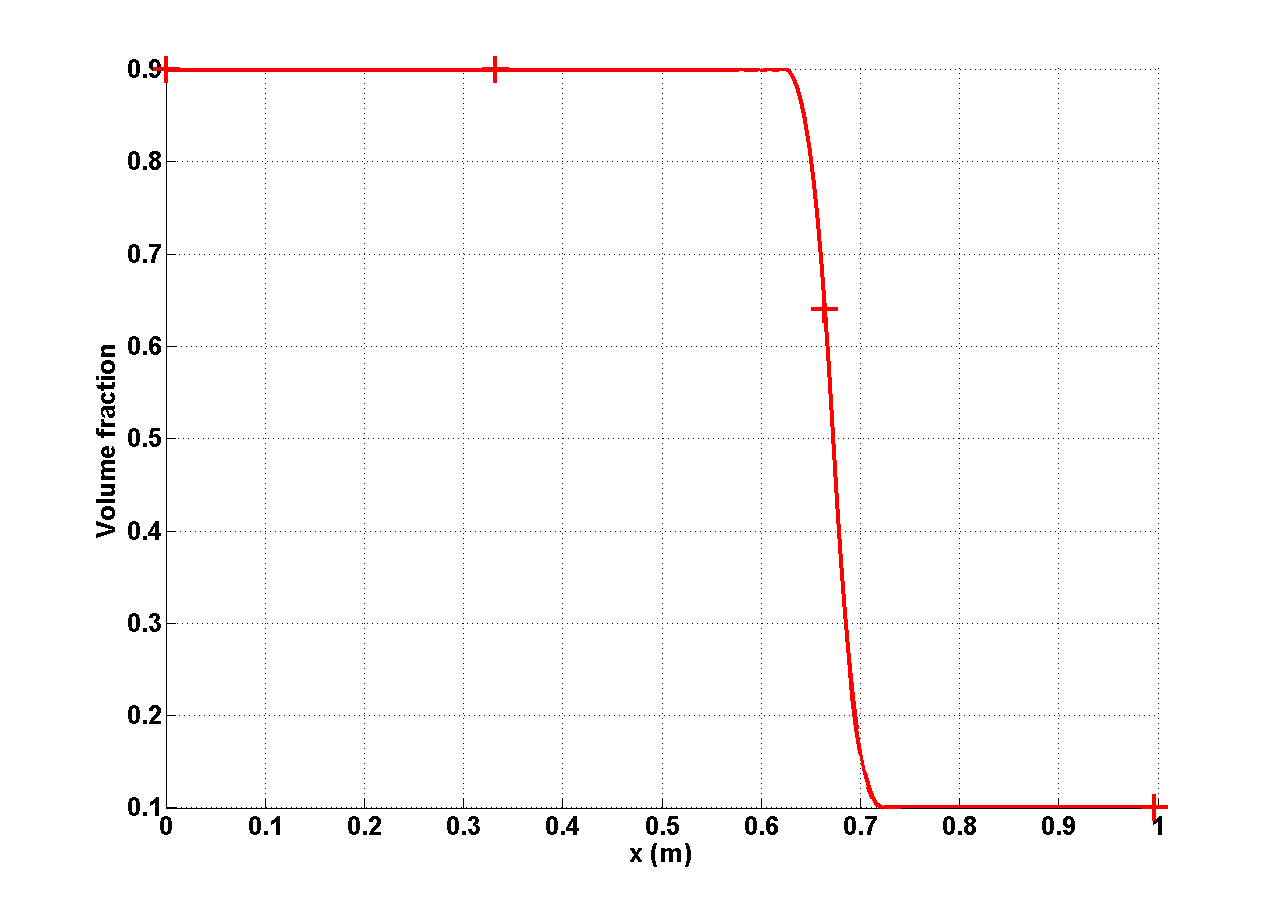
\includegraphics[width=\textwidth]{figures/SEM/liquid_volume_fraction.png}
%                \caption{Volume fraction of phase 1.}
                \caption{\label{fig:vf-liq-7-eqn-sect4}}
        \end{subfigure}%
        \begin{subfigure}[b]{0.495\textwidth}
                \centering
                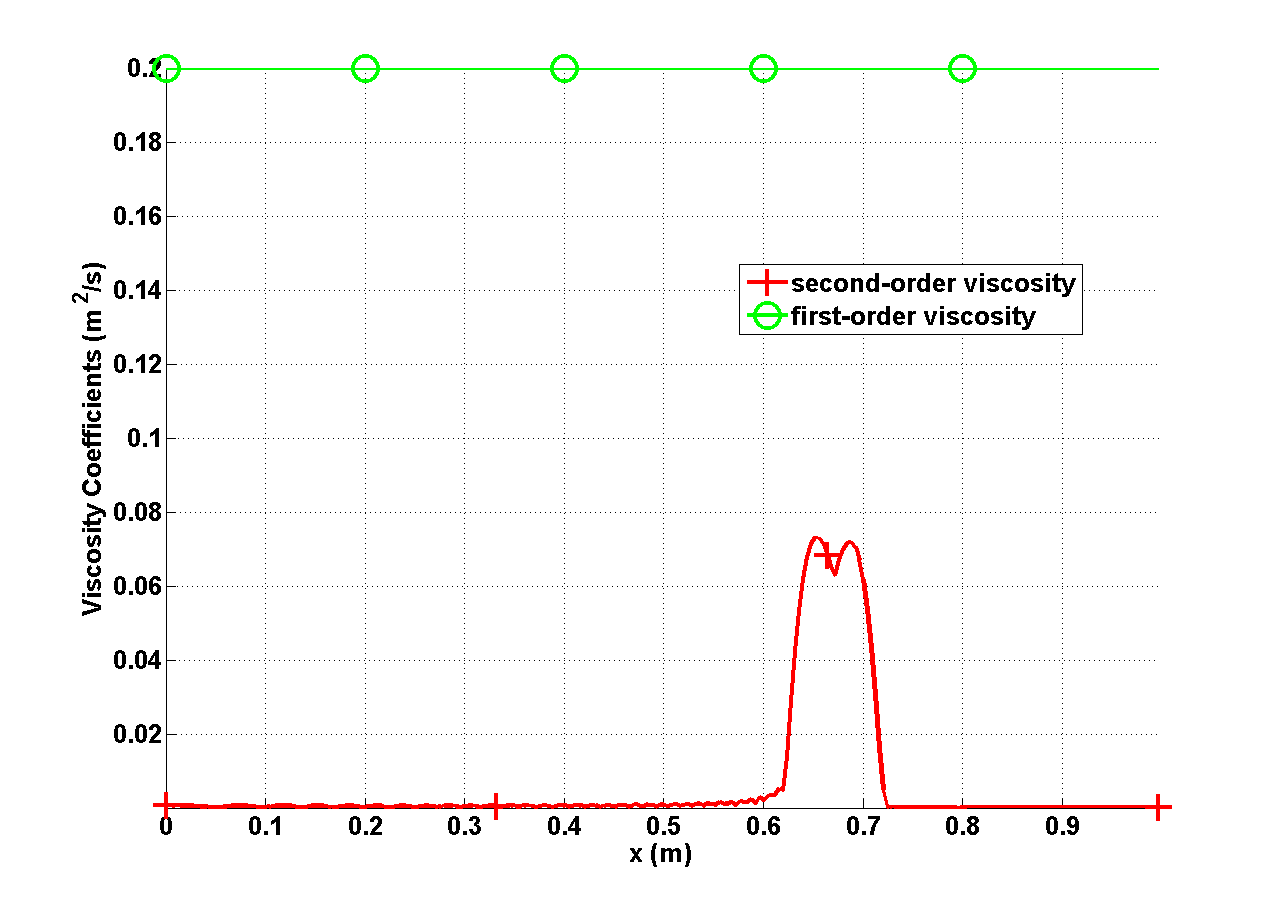
\includegraphics[width=\textwidth]{figures/SEM/liquid_beta.png}
%                \caption{Viscosity coefficients for volume fraction equation of phase 1.}
                \caption{\label{fig:beta-liq-7-eqn-sect4}}
        \end{subfigure}
        \caption{Volume fraction (left) and viscosity coefficients for volume fraction equation (right) of phase 1\label{fig:beta-visc-7-sect4}}
\end{figure}
%
\begin{figure}[H]
        \centering
        \begin{subfigure}[b]{0.495\textwidth}
                \centering
                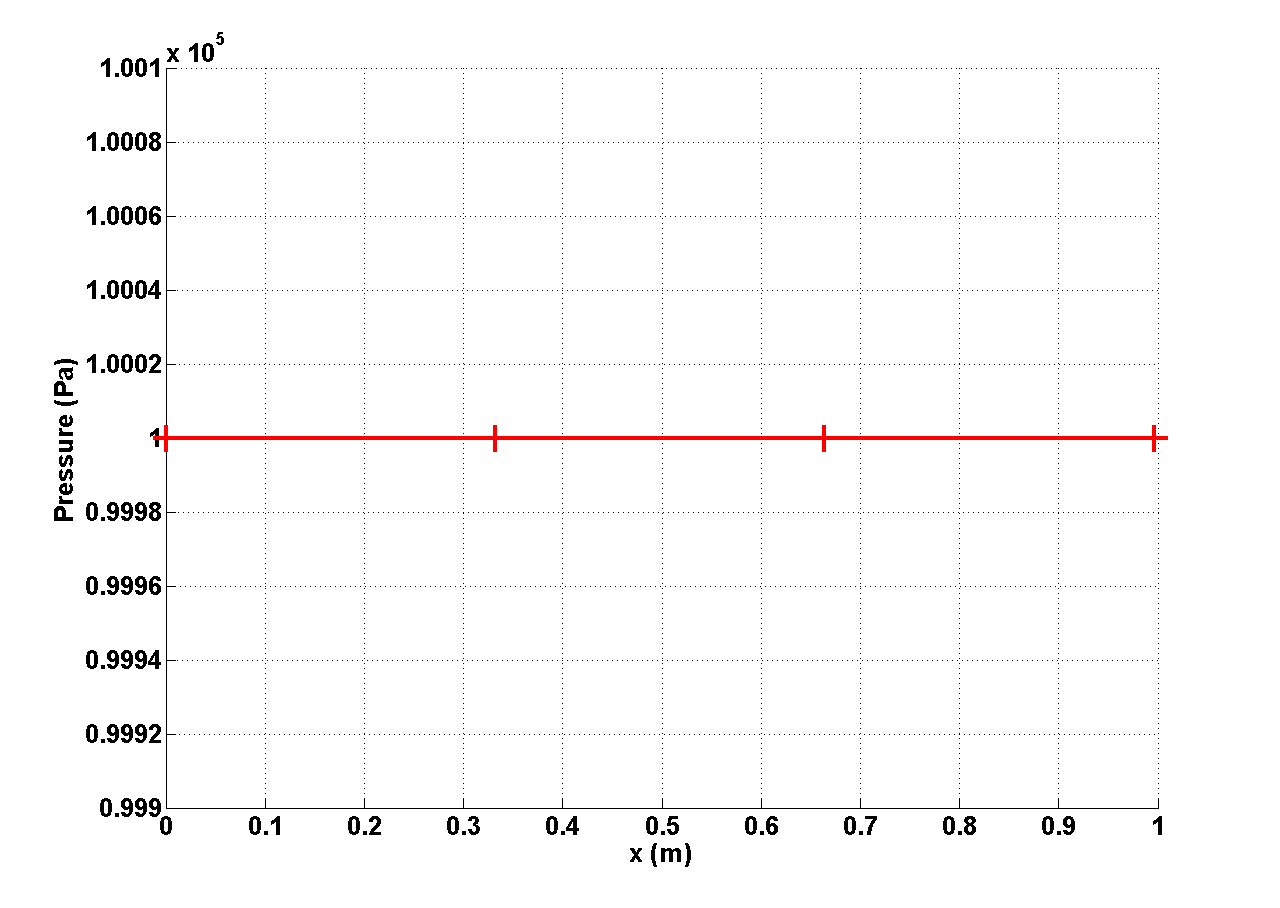
\includegraphics[width=\textwidth]{figures/SEM/liquid_pressure.png}
%                \caption{Pressure of phase 1.}
                \caption{\label{fig:press-1-7-eqn-sect4}}
        \end{subfigure}%
        \begin{subfigure}[b]{0.495\textwidth}
                \centering
                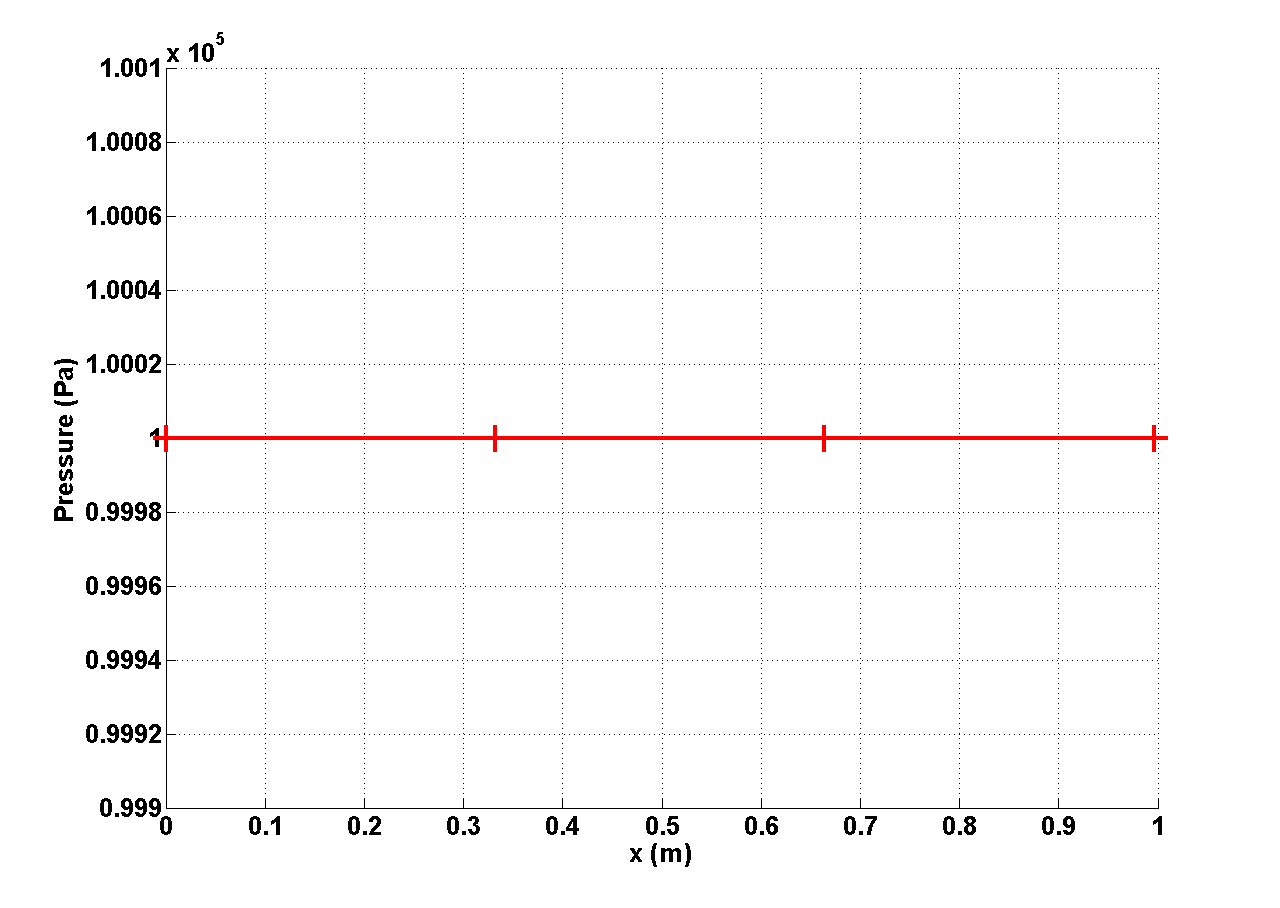
\includegraphics[width=\textwidth]{figures/SEM/vapor_pressure.png}
%                \caption{Pressure of phase $2$.}
                \caption{\label{fig:press-2-7-eqn-sect4}}
        \end{subfigure}
        \caption{Pressure profiles of phase $1$ (left) and $2$ (right)\label{fig:press-7-sect4}}
\end{figure}
%
\begin{figure}[H]
        \centering
        \begin{subfigure}[b]{0.495\textwidth}
                \centering
                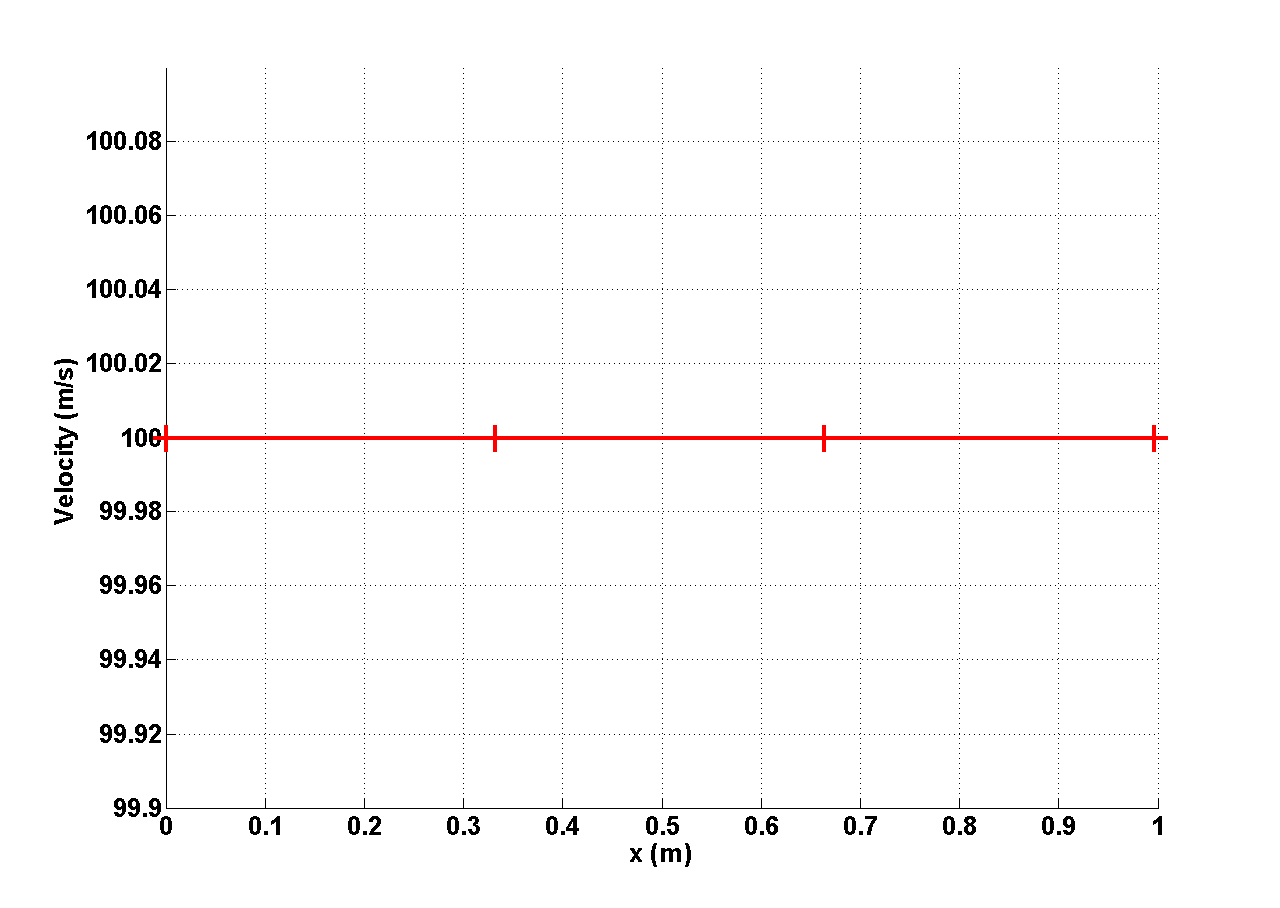
\includegraphics[width=\textwidth]{figures/SEM/liquid_velocity.png}
%                \caption{Velocity of phase 1.}
                \caption{\label{ig:vel-1-7-eqn-sect4}}
        \end{subfigure}%
        \begin{subfigure}[b]{0.495\textwidth}
                \centering
                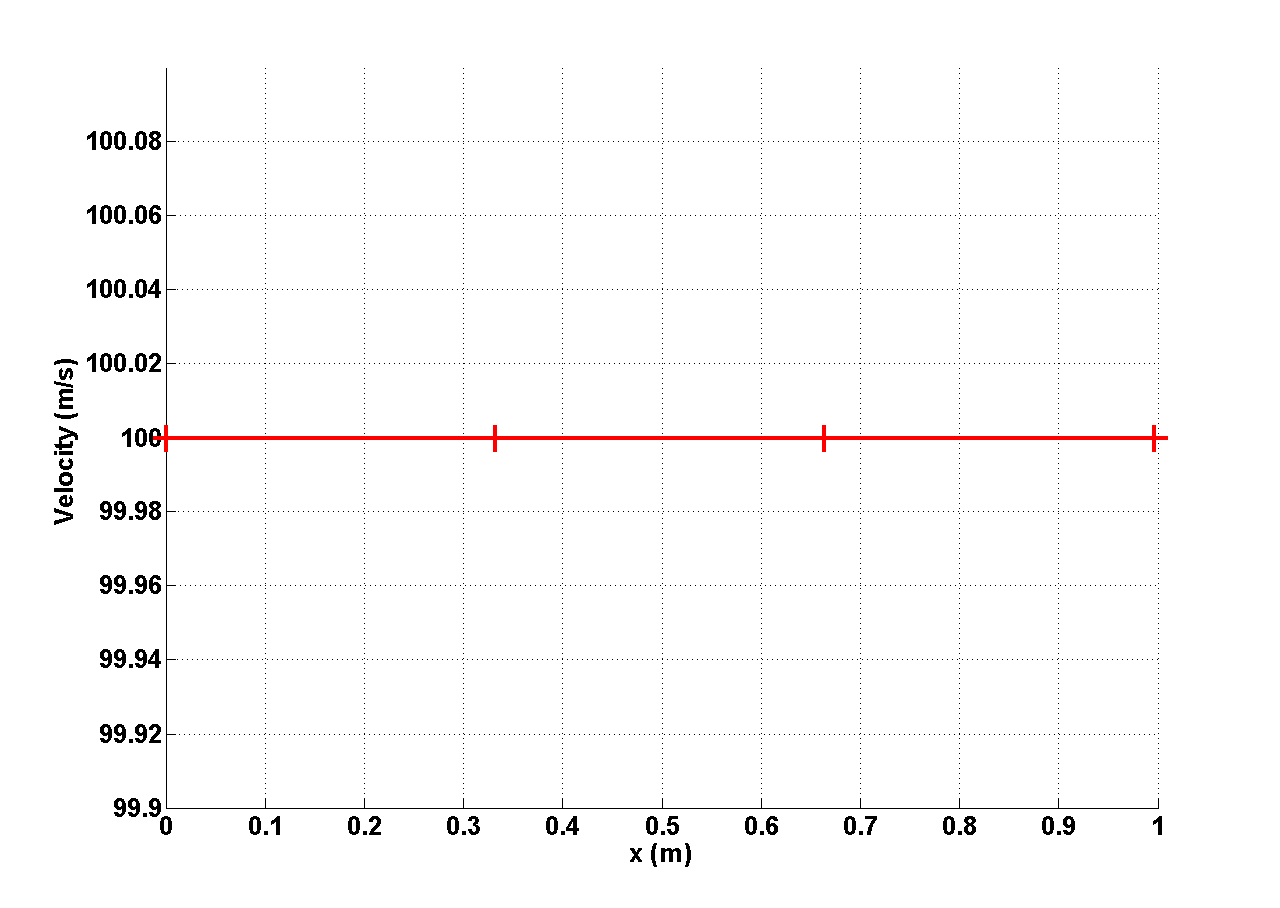
\includegraphics[width=\textwidth]{figures/SEM/vapor_velocity.png}
%                \caption{Velocity of phase $2$.}
                \caption{\label{ig:vel-2-7-eqn-sect4}}
        \end{subfigure}
        \caption{Velocity profiles of phase $1$ (left) and $2$ (right)\label{fig:vel-7-sect4}}
\end{figure}
%
\begin{figure}[H]
        \centering
        \begin{subfigure}[b]{0.495\textwidth}
                \centering
                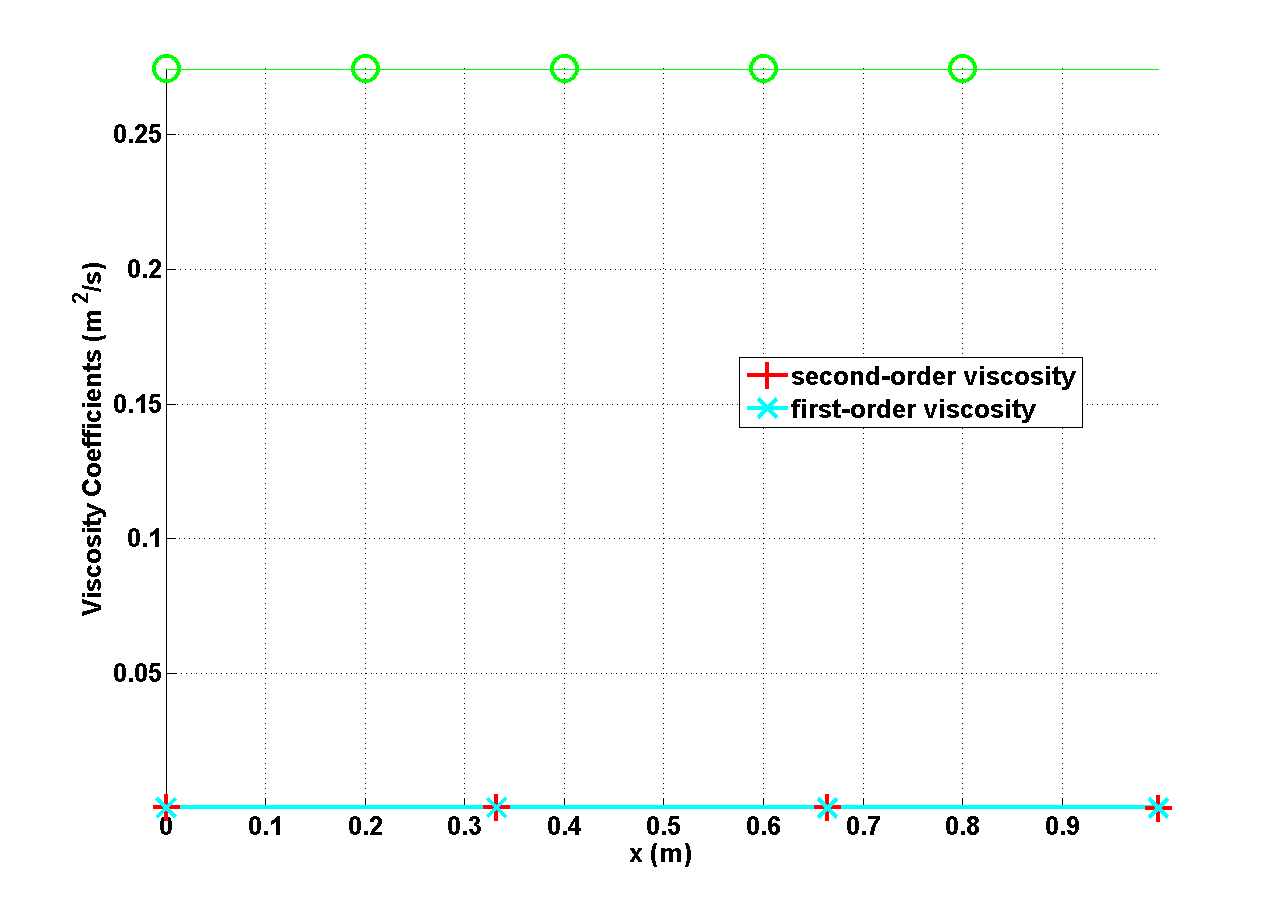
\includegraphics[width=\textwidth]{figures/SEM/liquid_viscosity.png}
%                \caption{Viscosity coefficients of phase 1.}
                \caption{\label{ig:visc-1-7-eqn-sect4}}
        \end{subfigure}%
        \begin{subfigure}[b]{0.495\textwidth}
                \centering
                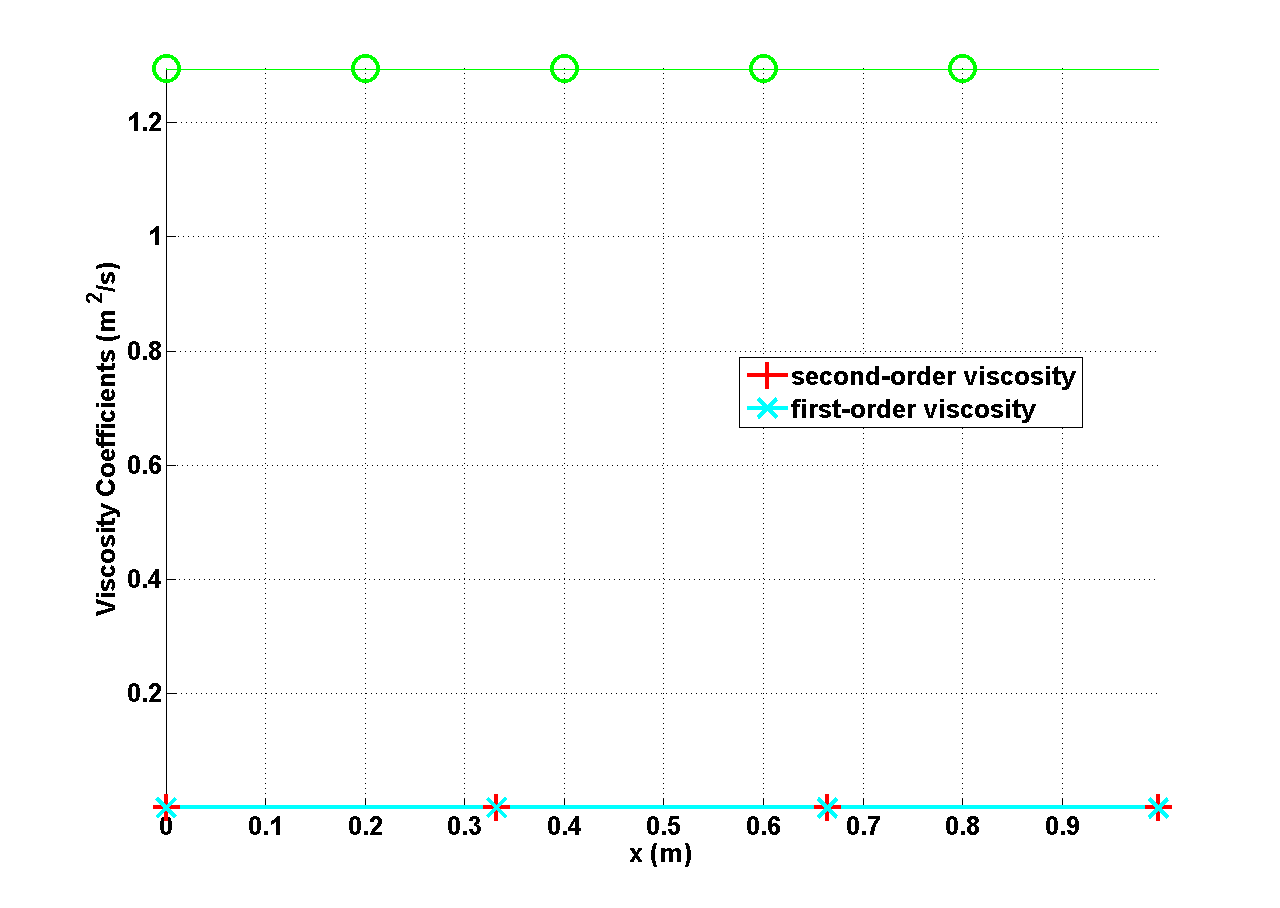
\includegraphics[width=\textwidth]{figures/SEM/vapor_viscosity.png}
%                \caption{Viscosity coefficients of phase $2$.}
                \caption{\label{fig:visc-2-7-eqn-sect4}}
        \end{subfigure}
        \caption{Viscosity coefficient profiles of phase $1$ (left) and $2$ (right)\label{fig:visc-7-sect4}}
\end{figure}
%
The stabilization numerical method preserves the uniform pressure (\fig{fig:press-7-sect4}) and velocity (\fig{fig:vel-7-sect4}) flow conditions while correctly resolving the discontinuity in the volume fraction profile as shown in \fig{fig:vf-liq-7-eqn-sect4}. The viscosity coefficients $\mu_k$ and $\kappa_k$ are equal to zero for both phases as shown in \fig{fig:visc-7-sect4}, since the flow conditions are uniform. However, the viscosity coefficient $\beta_k$ is peaked in the discontinuity region as expected. This test clearly shows that the stabilization method does not induce any artificial waves due to the smearing of the discontinuity in the volume fraction profile.
%-------------------------------------------------------------------------------------------------------------------------------------------------
\subsection{1-D shock tube for two independent fluids}\label{sec:1d-2-ind-phases-7-eq-sct4}
%-------------------------------------------------------------------------------------------------------------------------------------------------
We still consider a 1-D straight pipe of length $L=1$ $m$ filled with the same fluids as in \sect{sec:1d-advection-7-eq-sct4}. The membrane separates the pipe in two chambers with a high pressure ($P_{left} = 1$ $MPa$) on the left side and a low pressure ($P_{left} = 0.1$ $MPa$) in the right side. Both fluids are initially at rest. The volume fraction is set to $0.5$ which means each side of the chamber contains a mixture of two fluids with different equation of state parameters. Since the velocity and pressure relaxation coefficients $\mu_P$ and $\lambda_u$ are set to zero, the two fluids will behave independently to each other and the volume fraction is expected to remain uniform during the simulation. An exact solution is available for each fluid which simply corresponds to the single-phase exact solution obtained from a Riemann solver. The geometry is discretized with an uniform mesh of 500 cells and run with a $CFL$ of one until $t_{final} = 305$ $\mu s$. The numerical and exact solutions are given from \fig{fig:two-indep-fluids-press-7-eqn-sect4} to \ref{fig:two-indep-fluids-vf-visc-1-7-eqn-sect4}.
%
\begin{figure}[H]
\centering
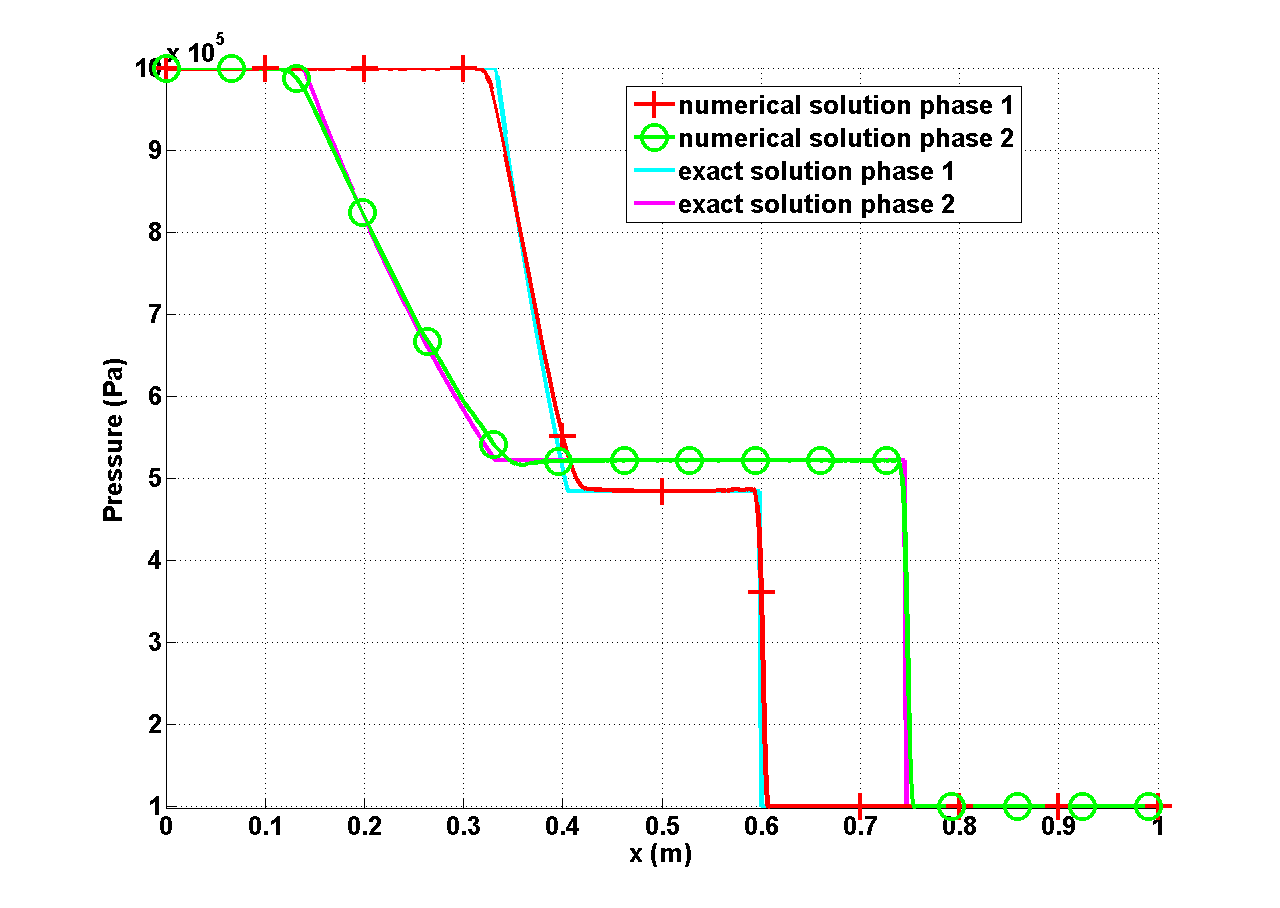
\includegraphics[width=\textwidth]{figures/SEM/two_phases_pressure.png}
\caption{Pressure profiles at $t=305$ $\mu s$.}
\label{fig:two-indep-fluids-press-7-eqn-sect4}
\end{figure}
%
\begin{figure}[H]
\centering
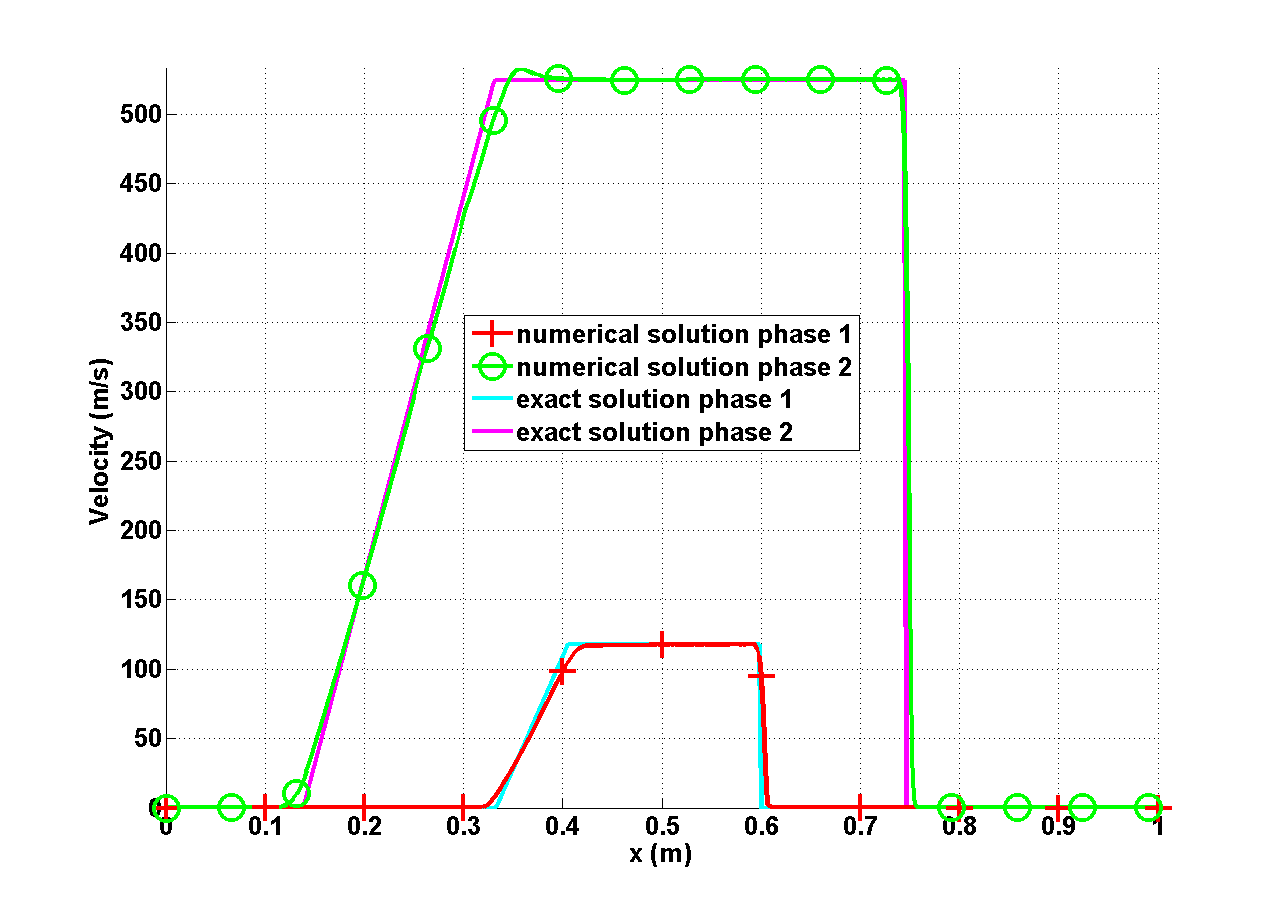
\includegraphics[width=\textwidth]{figures/SEM/two_phases_velocity.png}
\caption{Velocity profiles at $t=305$ $\mu s$.}
\label{fig:two-indep-fluids-vel-7-eqn-sect4}
\end{figure}
%
\begin{figure}[H]
\centering
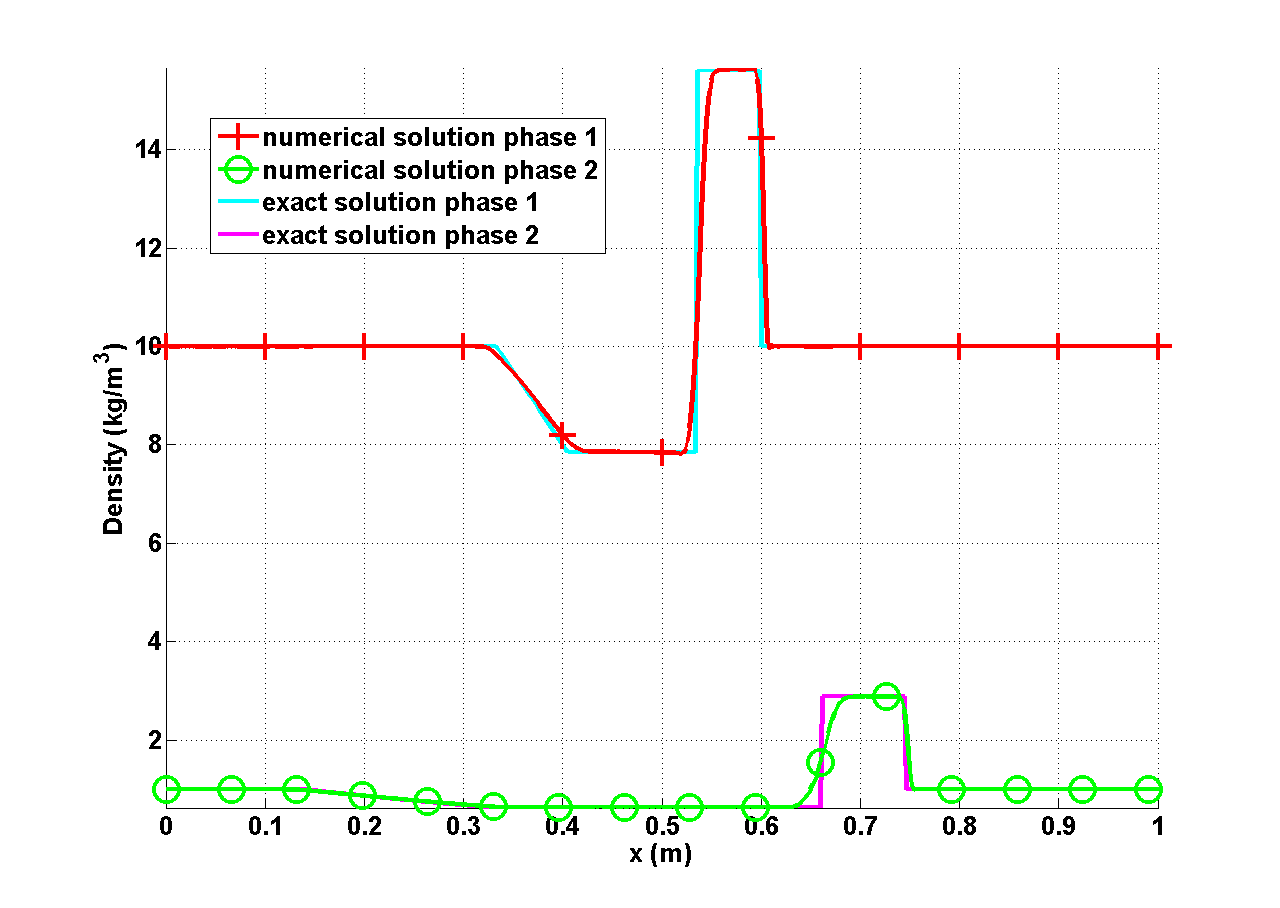
\includegraphics[width=\textwidth]{figures/SEM/two_phases_density.png}
\caption{Density profiles at $t=305$ $\mu s$.}
\label{fig:two-indep-fluids-dens-7-eqn-sect4}
\end{figure}
%
\begin{figure}[H]
\centering
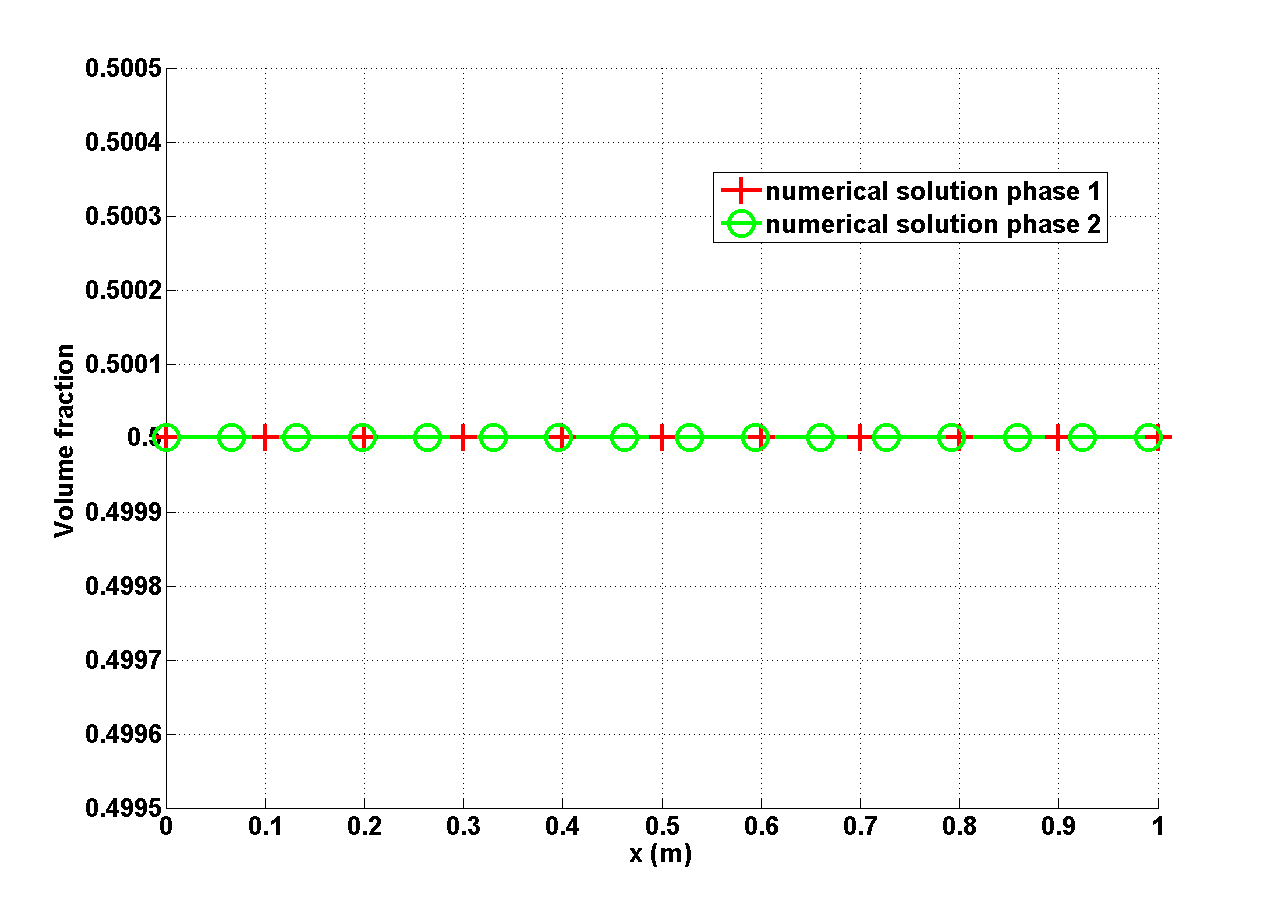
\includegraphics[width=\textwidth]{figures/SEM/two_phases_volume_fraction.png}
\caption{Volume fraction profiles at $t=305$ $\mu s$.}
\label{fig:two-indep-fluids-vf-7-eqn-sect4}
\end{figure}
%
\begin{figure}[H]
\centering
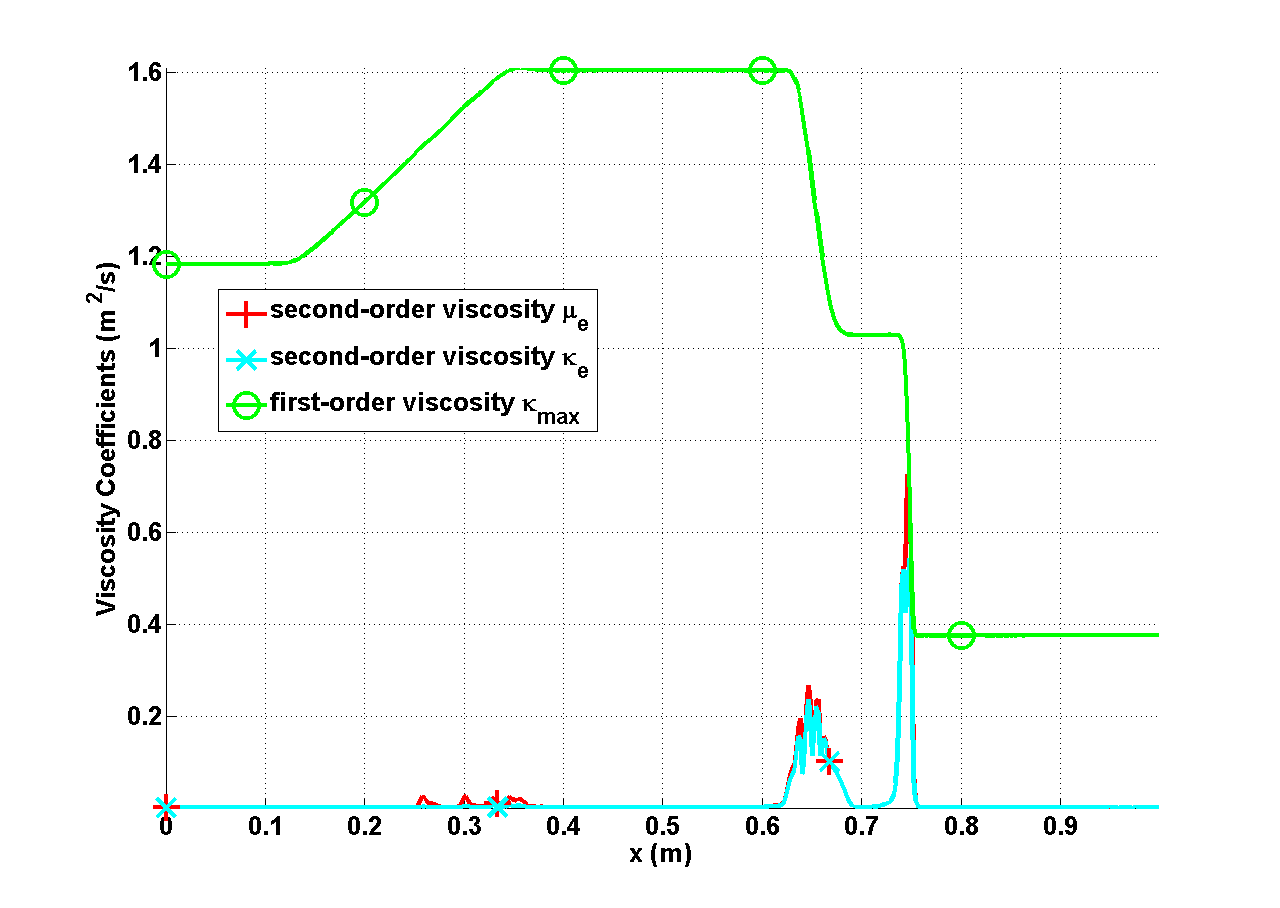
\includegraphics[width=\textwidth]{figures/SEM/two_phases_liquid_viscosity_kappa_mu.png}
\caption{Viscosity coefficient profiles for phase $2$ at $t=305$ $\mu s$.}
\label{fig:two-indep-fluids-visc-2-7-eqn-sect4}
\end{figure}
%
\begin{figure}[H]
\centering
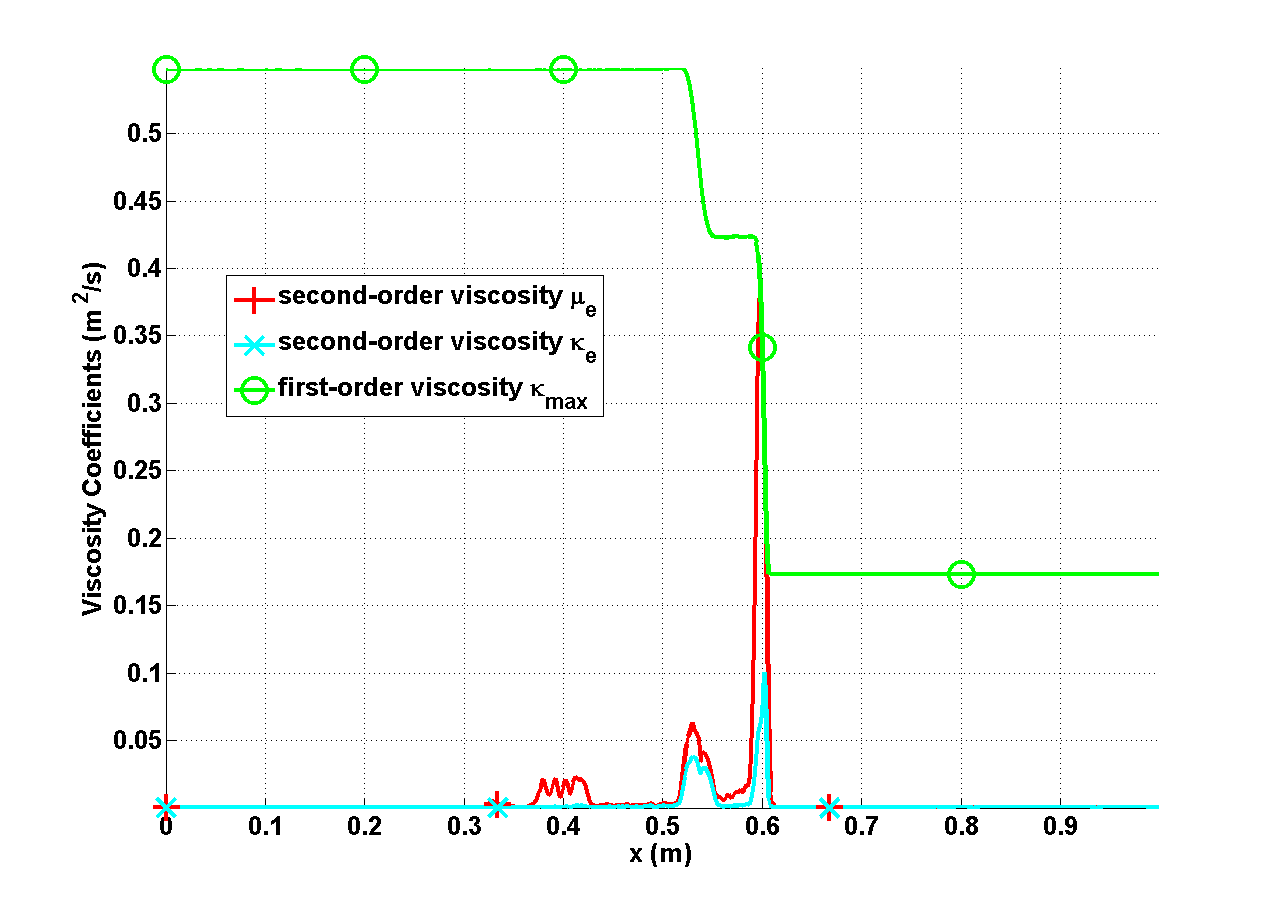
\includegraphics[width=\textwidth]{figures/SEM/two_phases_vapor_viscosity_kappa_mu.png}
\caption{Viscosity coefficient profiles for phase 1 at $t=305$ $\mu s$.}
\label{fig:two-indep-fluids-visc-1-7-eqn-sect4}
\end{figure}
%
\begin{figure}[H]
\centering
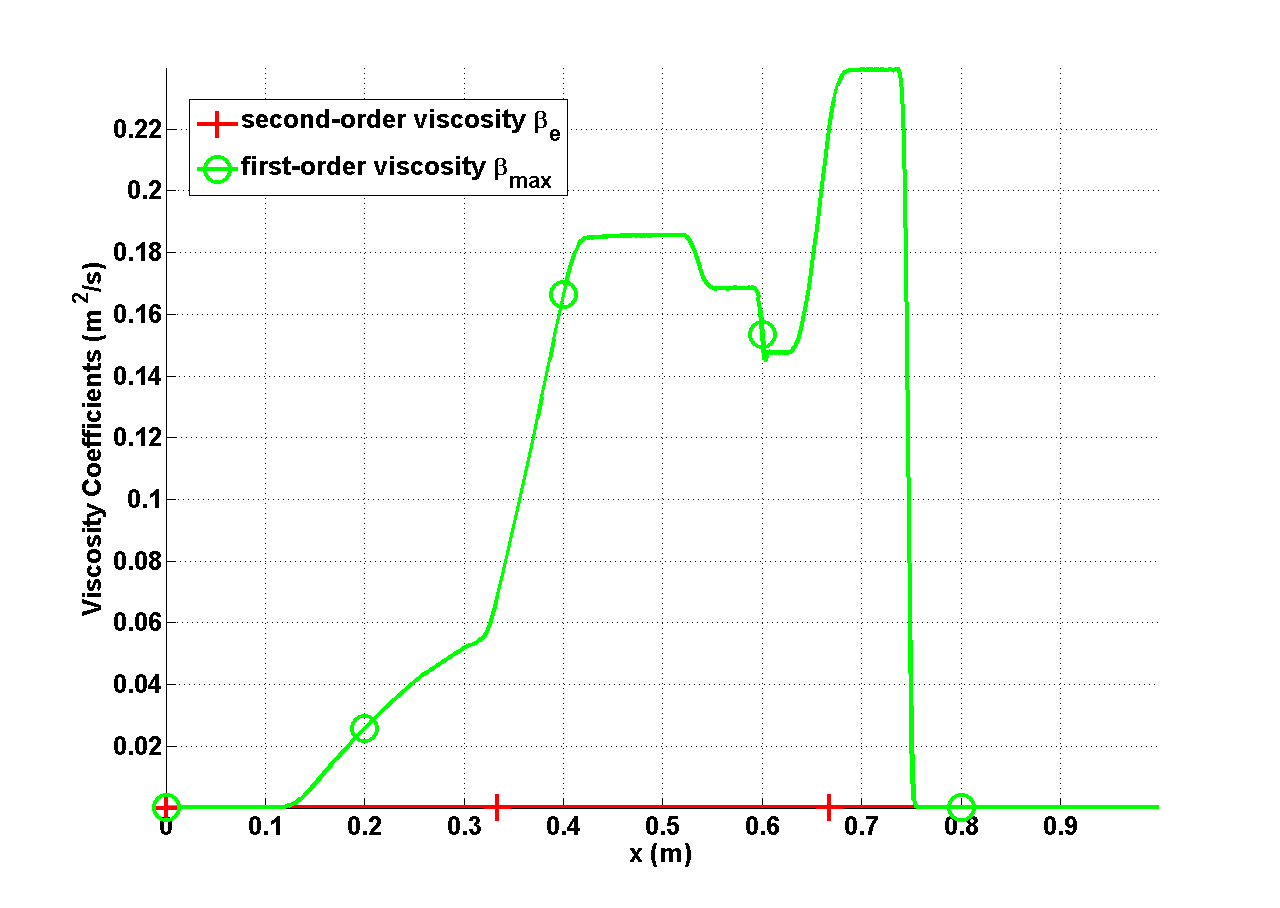
\includegraphics[width=\textwidth]{figures/SEM/two_phases_liquid_beta.png}
\caption{Viscosity coefficient profiles for volume fraction equation of phase 1 at $t=305$ $\mu s$.}
\label{fig:two-indep-fluids-vf-visc-1-7-eqn-sect4}
\end{figure}
%
The pressure, velocity and density profiles given in \fig{fig:two-indep-fluids-press-7-eqn-sect4}, \fig{fig:two-indep-fluids-vel-7-eqn-sect4} and \fig{fig:two-indep-fluids-dens-7-eqn-sect4}, respectively, show good agreement with the exact solutions for both phases. The fluid $2$ is lighter and thus experiences stronger variations: its velocity is larger and the shock moves faster. The viscosity coefficients shown in \fig{fig:two-indep-fluids-visc-2-7-eqn-sect4} and \fig{fig:two-indep-fluids-visc-1-7-eqn-sect4} for both phases have similar profiles: they are peaked in the shock regions and also display a bump in the contact wave. In \fig{fig:two-indep-fluids-vf-7-eqn-sect4}, it is noted that the volume fraction profiles remain uniform and are not altered by the variations in the other variables. The viscosity coefficient $\beta_k$ used in the volume fraction equation is zero (\fig{fig:two-indep-fluids-vf-visc-1-7-eqn-sect4}) as expected since the volume fraction profile is uniform.
%-------------------------------------------------------------------------------------------------------------------------------------------------
\subsection{1-D shock tube for two fluids with pressure and velocity relaxation terms}\label{sec:1d-2-phases-rel-7-eq-sct4}
%-------------------------------------------------------------------------------------------------------------------------------------------------
Once again, we consider a 1-D shock tube with the same initial conditions and the same fluids as in \sect{sec:1d-2-ind-phases-7-eq-sct4}. The pressure and velocity relaxation coefficients are no longer set to zero but computed from \eqt{E-R:85} and \eqt{E-R:86} with $A_{int,max} =  10^4$ $m^{-1}$: $\mu_P \sim 4$ and $\lambda_u \sim 5 \times 10^5$ $s^{-1}$. The values of the relaxation coefficients are large enough to make the relaxation terms dominant in the momentum and energy equations of each phase (see \eqt{eq:liq-7-eqn-sect5} and \eqt{eq:vap-7-eqn-sect5}). Thus, the two fluids will exhibit the same pressure and velocity. The volume fraction will not remain uniform but is expected to vary due to the pressure relaxation source term (\eqt{eqn:multi-d-7-eqn-liq-vol}). For this test, an exact solution is not available but the reader can refer to \cite{Saurel_2007} for a comparison. An uniform mesh of 500 cells is used. The code is run until $t_{final} = 305$ $\mu s$ with a $CFL$ of one. The numerical solutions are presented in \fig{fig:two-fluids-rel-press-7-eqn-sect4} to \ref{fig:two-fluids-rel-vf-visc-1-7-eqn-sect4}.
%
\begin{figure}[H]
\centering
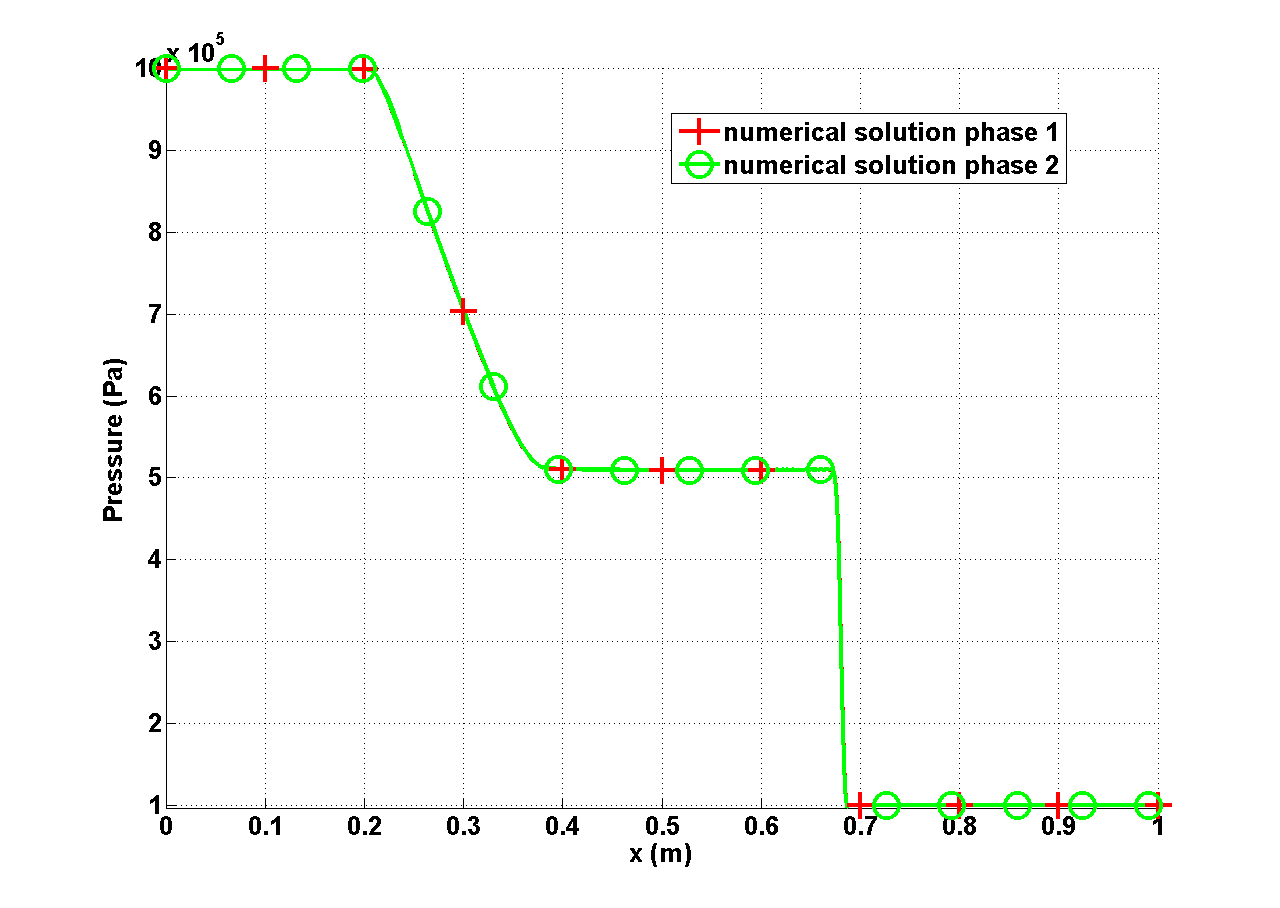
\includegraphics[width=\textwidth]{figures/SEM/relaxation_two_phases_pressure.png}
\caption{Pressure profiles at $t=305$ $\mu s$.}
\label{fig:two-fluids-rel-press-7-eqn-sect4}
\end{figure}
%
\begin{figure}[H]
\centering
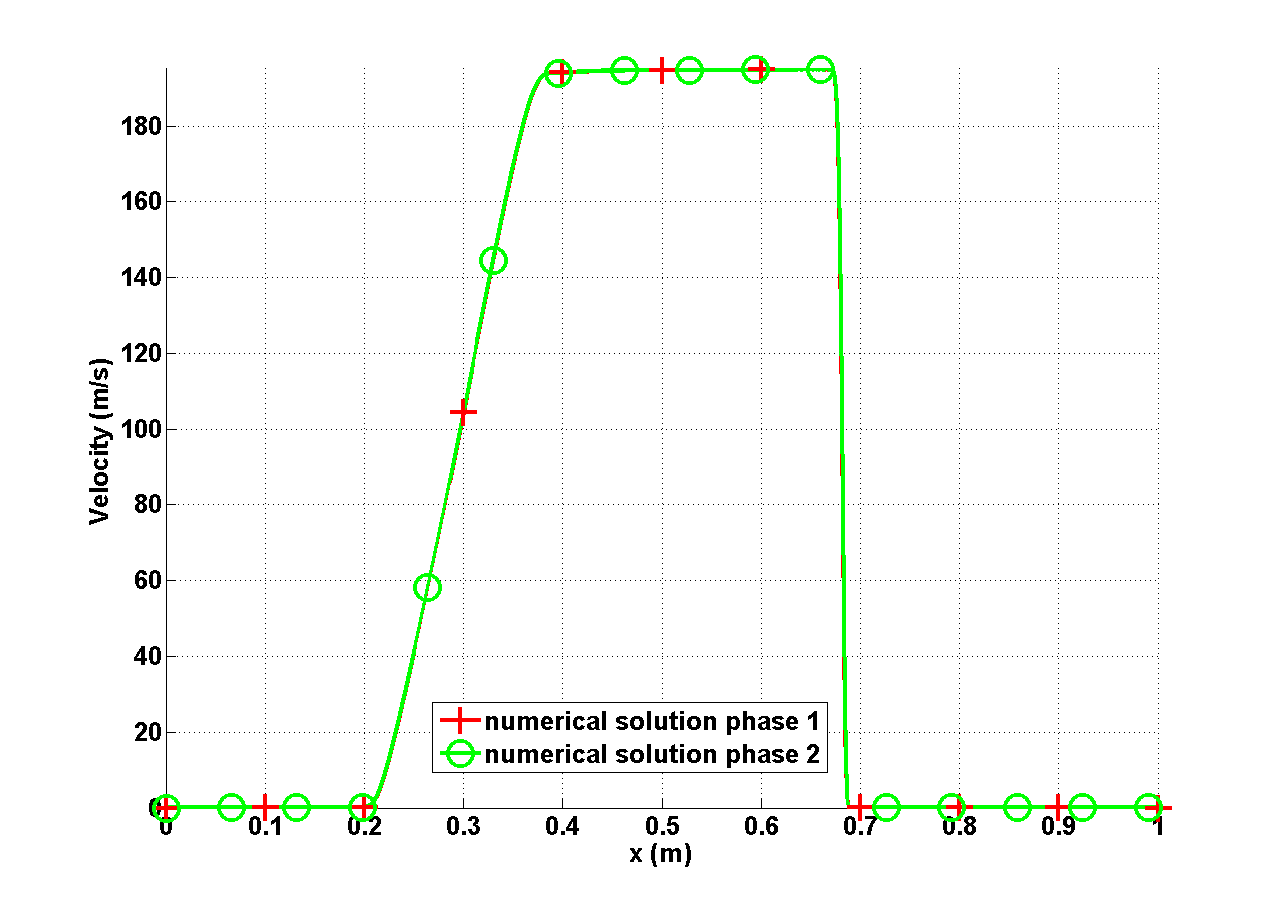
\includegraphics[width=\textwidth]{figures/SEM/relaxation_two_phases_velocity.png}
\caption{Velocity profiles at $t=305$ $\mu s$.}
\label{fig:two-fluids-rel-vel-7-eqn-sect4}
\end{figure}
%
\begin{figure}[H]
\centering
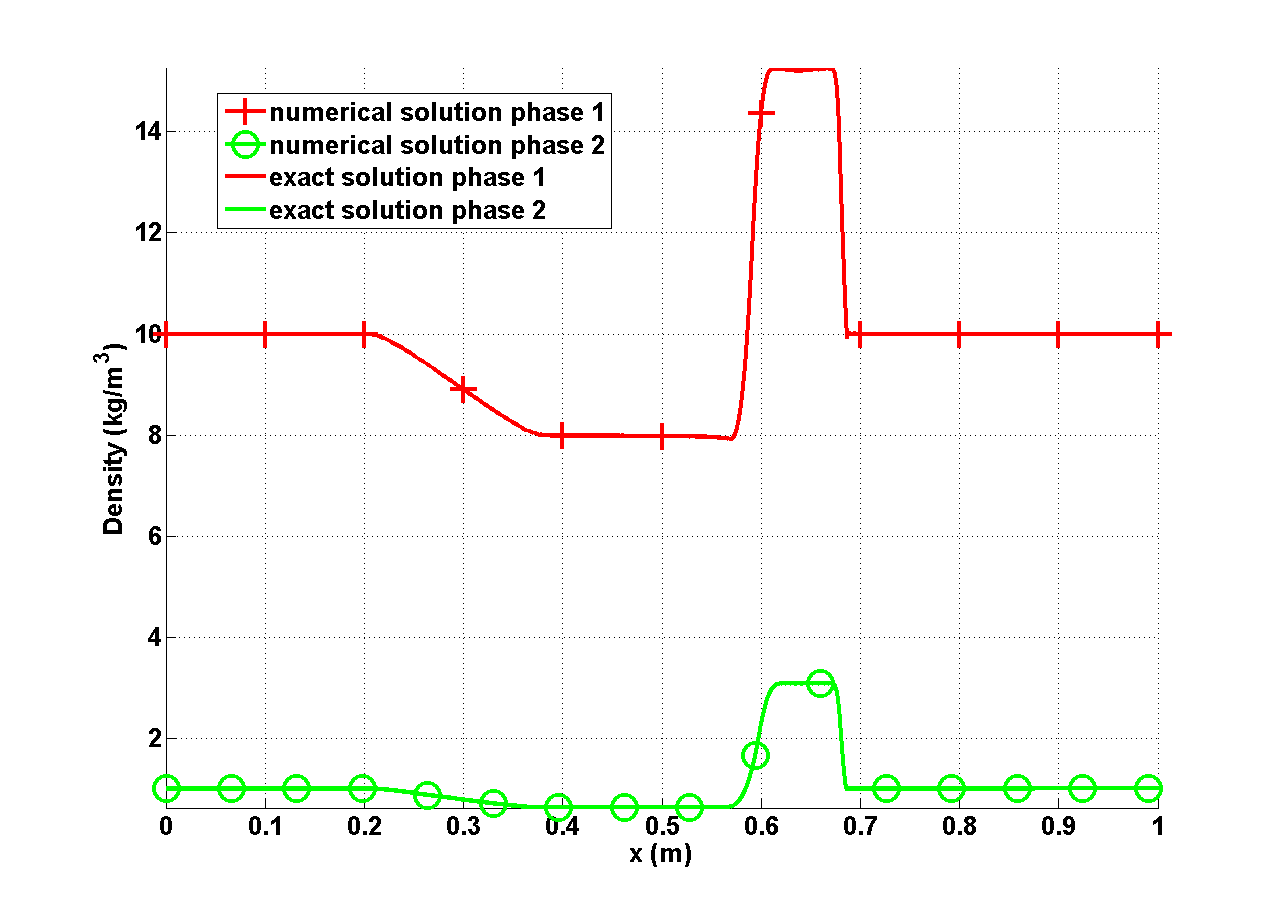
\includegraphics[width=\textwidth]{figures/SEM/relaxation_two_phases_density.png}
\caption{Density profiles at $t=305$ $\mu s$.}
\label{fig:two-fluids-rel-rho-7-eqn-sect4}
\end{figure}
%
\begin{figure}[H]
\centering
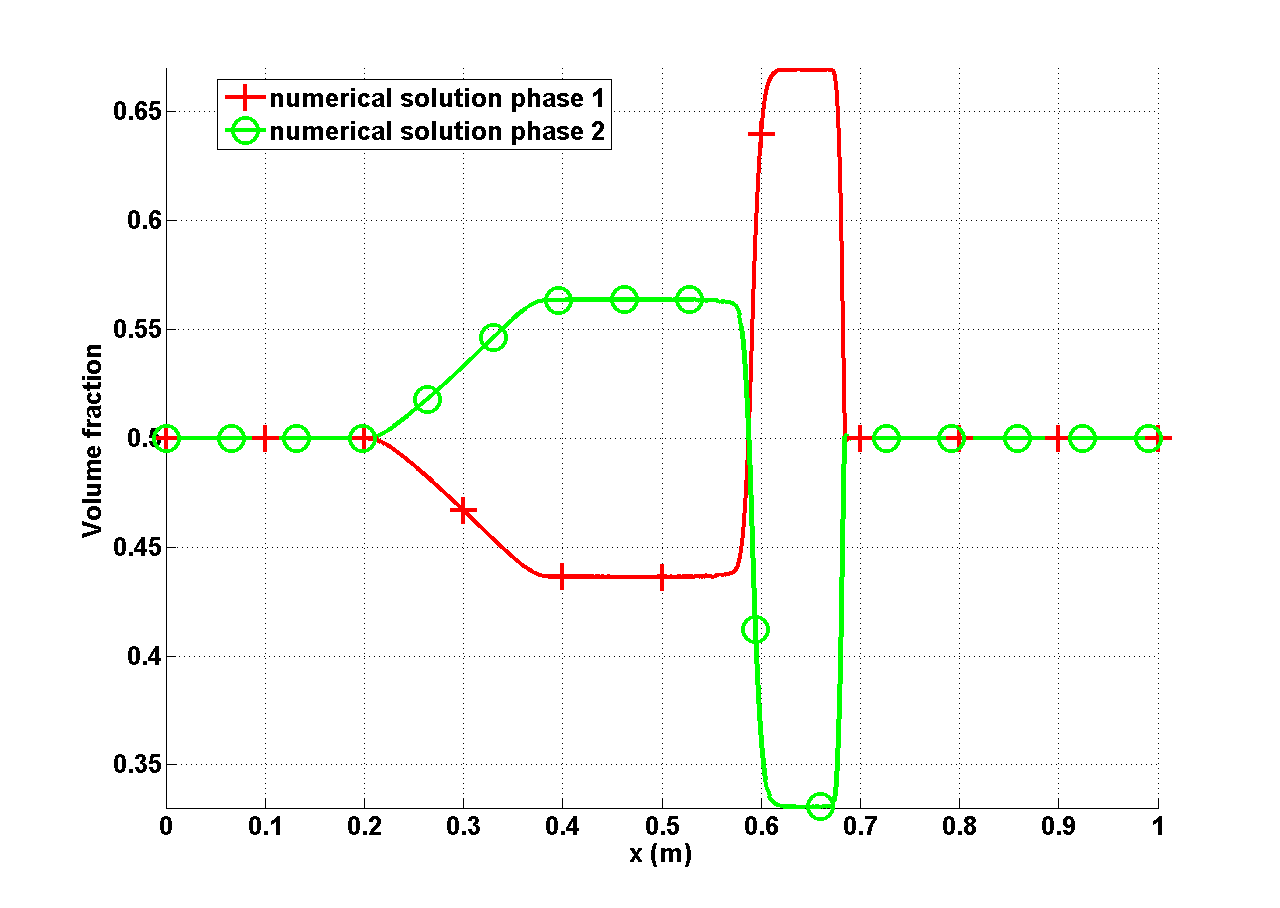
\includegraphics[width=\textwidth]{figures/SEM/relaxation_two_phases_volume_fraction.png}
\caption{Volume fraction profiles at $t=305$ $\mu s$.}
\label{fig:two-fluids-rel-vf-7-eqn-sect4}
\end{figure}
%
\begin{figure}[H]
\centering
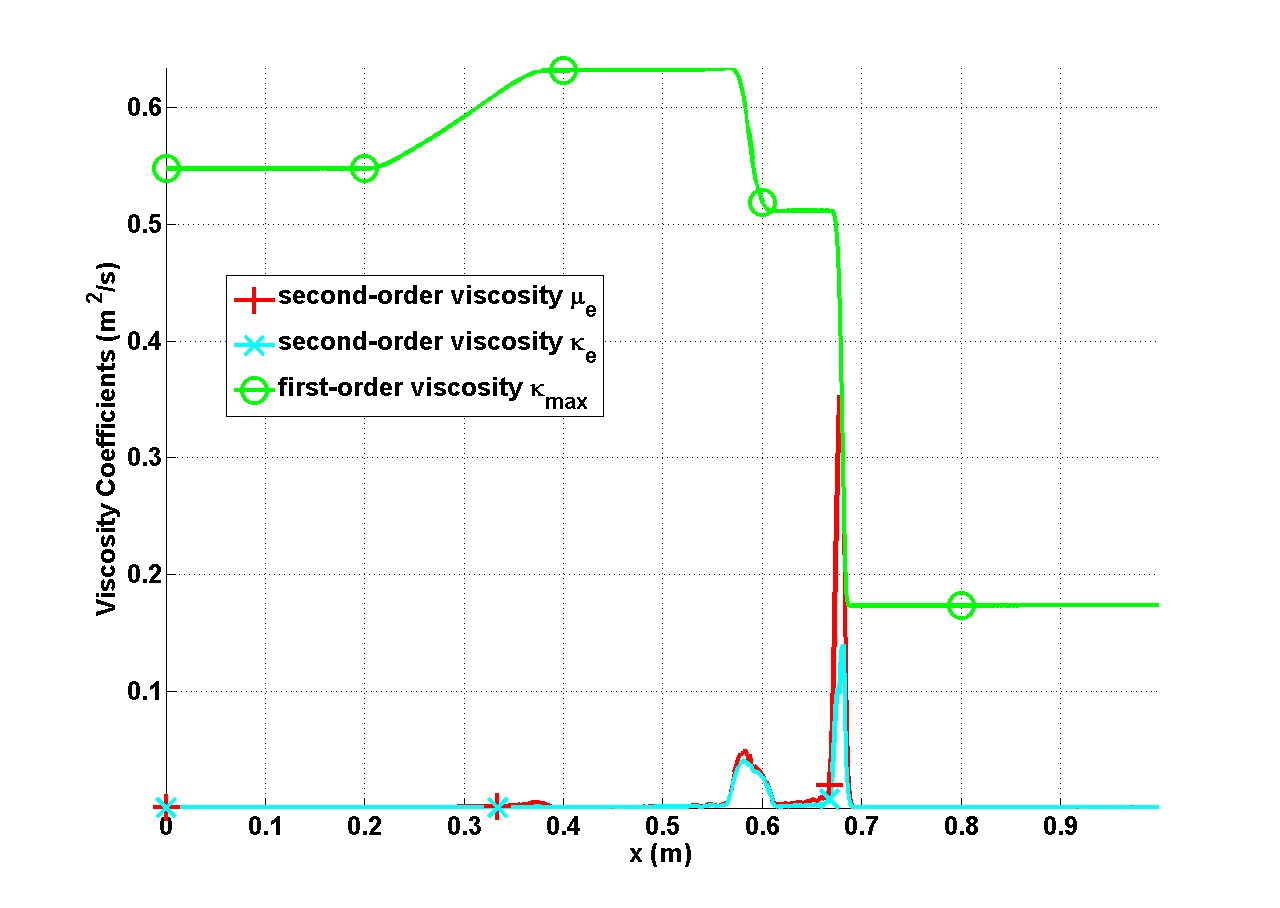
\includegraphics[width=\textwidth]{figures/SEM/relaxation_two_phases_liquid_viscosity_kappa_mu.png}
\caption{Viscosity coefficient profiles for phase 1 at $t=305$ $\mu s$.}
\label{fig:two-fluids-rel-visc-2-7-eqn-sect4}
\end{figure}
%
\begin{figure}[H]
\centering
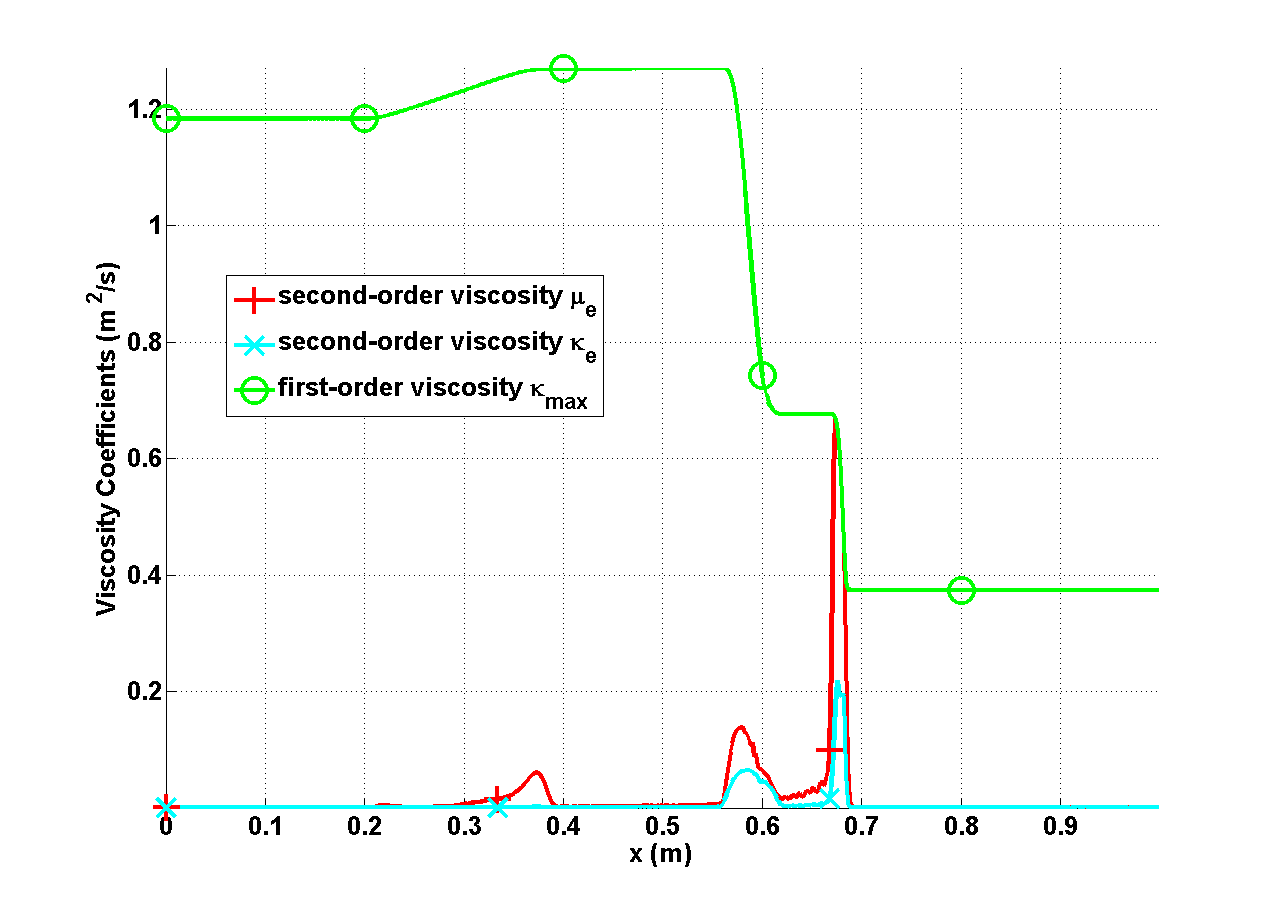
\includegraphics[width=\textwidth]{figures/SEM/relaxation_two_phases_vapor_viscosity_kappa_mu.png}
\caption{Viscosity coefficient profiles for phase $2$ at $t=305$ $\mu s$.}
\label{fig:two-fluids-rel-visc-1-7-eqn-sect4}
\end{figure}
%
\begin{figure}[H]
\centering
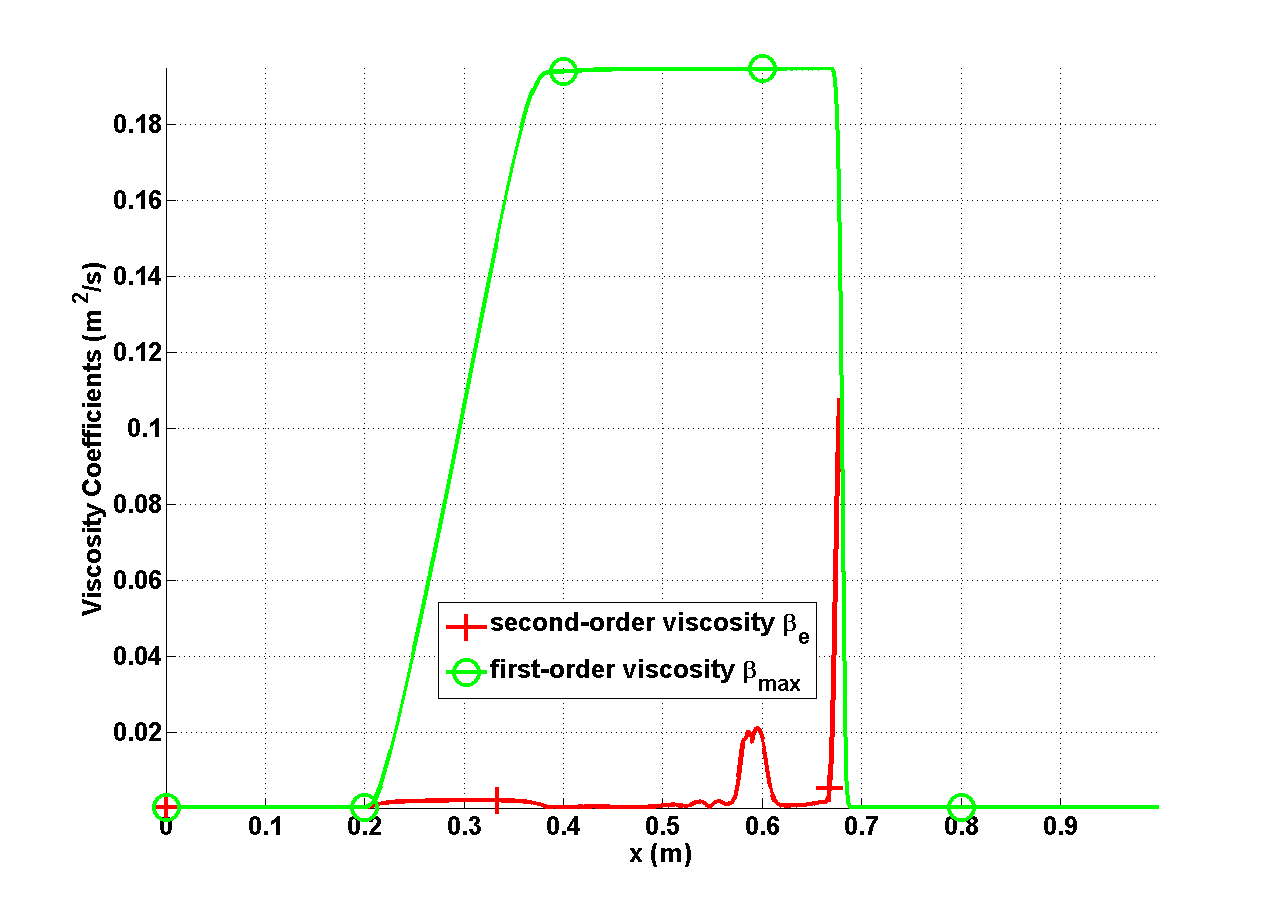
\includegraphics[width=\textwidth]{figures/SEM/relaxation_two_phases_liquid_beta.png}
\caption{Viscosity coefficient profiles for volume fraction equation of phase 1 at $t=305$ $\mu s$.}
\label{fig:two-fluids-rel-vf-visc-1-7-eqn-sect4}
\end{figure}
%
As expected, the two fluids have the same pressure and velocity profiles as shown in \fig{fig:two-fluids-rel-press-7-eqn-sect4} and \fig{fig:two-fluids-rel-vel-7-eqn-sect4}, respectively. The shock is well resolved and does not display any instability. The main difference with the numerical results obtained in \sect{sec:1d-2-ind-phases-7-eq-sct4} lies in the volume fraction profiles that are no longer uniform but display a shock wave around $x=0.7$ $m$ as shown in \fig{fig:two-fluids-rel-vf-7-eqn-sect4}. Consequently, the viscosity coefficient $\beta_k$ is peaked in the same region.  
%-------------------------------------------------------------------------------------------------------------------------------------------------
\subsection{1-D converging-diverging nozzle test}\label{sec:1d-nozzle-rel-7-eq-sct4}
%-------------------------------------------------------------------------------------------------------------------------------------------------
In this test, we propose to investigate the behavior of two fluids in a one meter long 1-D converging-diverging nozzle with $A(x) = 1 + 0.5 \cos \left( 2\pi x \right)$. This test was first introduced by Saurel et al. in \cite{SEM} for the 1-D seven-equation model and consists of a mixture of liquid water and vapor described by the SGEOS with the parameters given in \tbl{tbl:stff_gas_eos-sect4}.
%
\begin{table}[H]
\begin{center}
\caption{ Stiffened Gas Equation of State (SGEOS) parameters for steam and liquid water.}
\label{tbl:stff_gas_eos-sect4}
\begin{tabular}{|c|c|c|c|c|}
 \hline
\text{fluid}                           & $\gamma$ & $C_v$ $(J.kg^{-1}.K^{-1})$ & $P_\infty$ $(Pa)$ & $q$ $(J.kg^{-1})$ \\  \hline \hline
liquid water & 2.35     & 1816                       & $10^9$            & $-1167\ 10^3$     \\  \hline
steam          & 1.43     & 1040                       & 0                 & $ 2030\ 10^3$     \\  \hline
\end{tabular}
\end{center}
\end{table}
%
Stagnation boundary conditions are specified on the left of the nozzle (inlet) for both phases with a stagnation temperature $T_0 = 453 $ $K$ and a stagnation pressure $P_0 = 1$ $MPa$ (the stagnation density can be computed from $T_0$ and $P_0$ and the equation of state). At the outlet, a static pressure boundary condition is specified with $P = 0.5$ $MPa$ for both phases. The volume fraction is set to $\alpha_k = 0.5$ at the inlet. The initial conditions are computed from the boundary conditions by assuming the two fluids at rest and linearly interpolating the pressure and temperature between the boundary values. The geometry is discretized with an uniform mesh of 100 cells and run until steady-state. The pressure and velocity relaxation coefficients are computed from \eqt{E-R:85} and \eqt{E-R:86} and the use of \eqt{eq:Aint-sect4} for different values of $A_{int,max}$ that will be specified. The reader can refer to \sect {sec:liquid_nozzle} and \sect{sec:steam_nozzle} for numerical solutions in a 1-D nozzle when considering two independent fluids (i.e., without relaxation source terms). First numerical results are presented when considering only the pressure and velocity relaxation terms for different values of $A_{int,max}$. Then, the same simulation is run when adding the mass and energy exchange source terms.

We first consider the 1-D seven-equation model with the relaxation source terms for different values of $A_{int,max} = 10^2 \text{, } 10^3$ and $10^4$ $m^{-1}$. The pressure profiles are given for all of the value of $A_{int,max}$ for comparison. The density, velocity, volume fraction and viscosity coefficients are only given for $A_{int,max} = 10^4$ $m^{-1}$. The numerical results are presented from \fig{fig:two-fluids-rel-nozzle-press-Aint4-sem-sect4} to \ref{fig:two-fluids-rel-nozzle-visc-vf-sem-sect4}.
%
\begin{figure}[H]
\centering
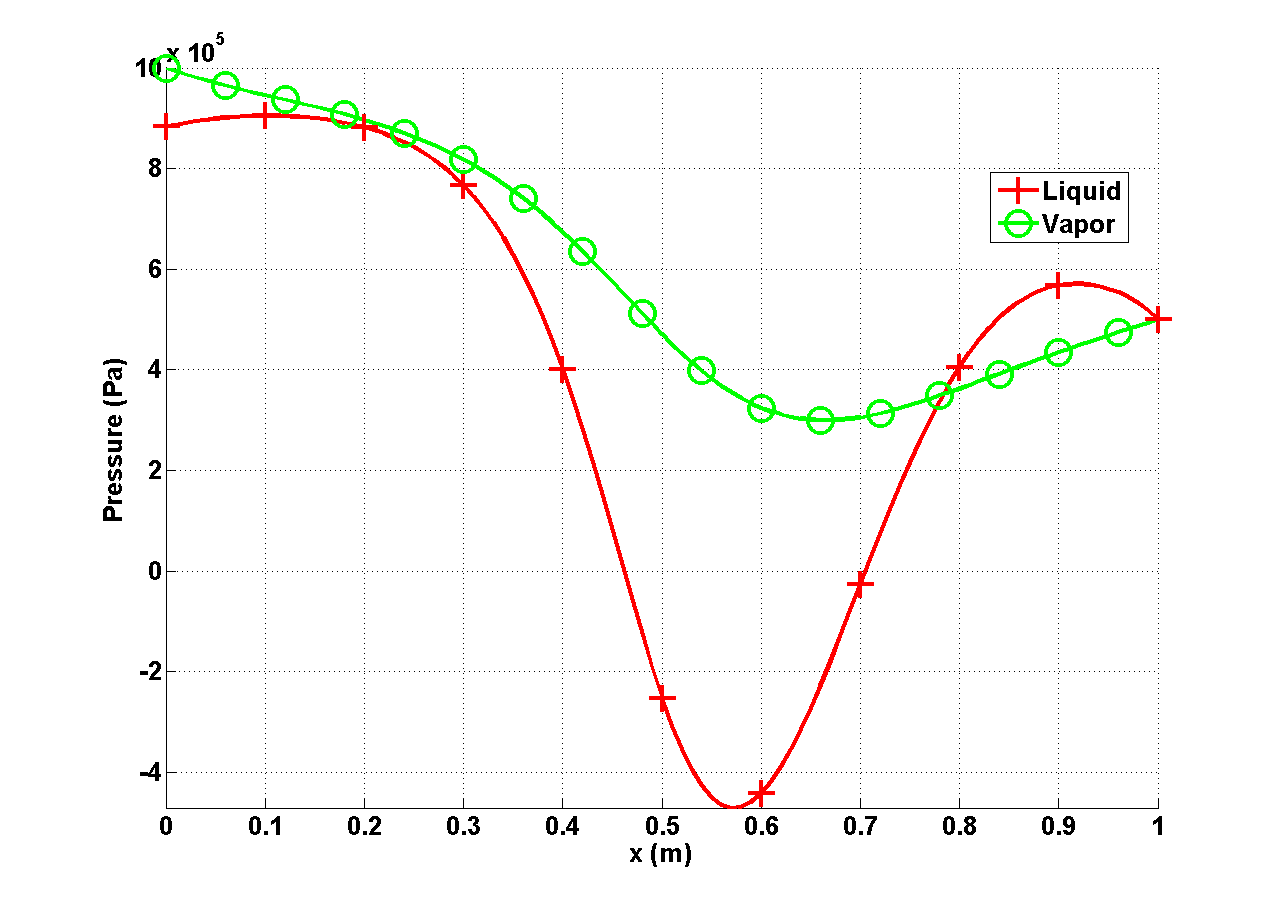
\includegraphics[width=\textwidth]{figures/SEM/Aint1e2_two_phases_pressure.png}
\caption{Pressure profiles at steady state with $A_{int,max} = 10^2$.}
\label{fig:two-fluids-rel-nozzle-press-Aint2-sem-sect4}
\end{figure}
%
\begin{figure}[H]
\centering
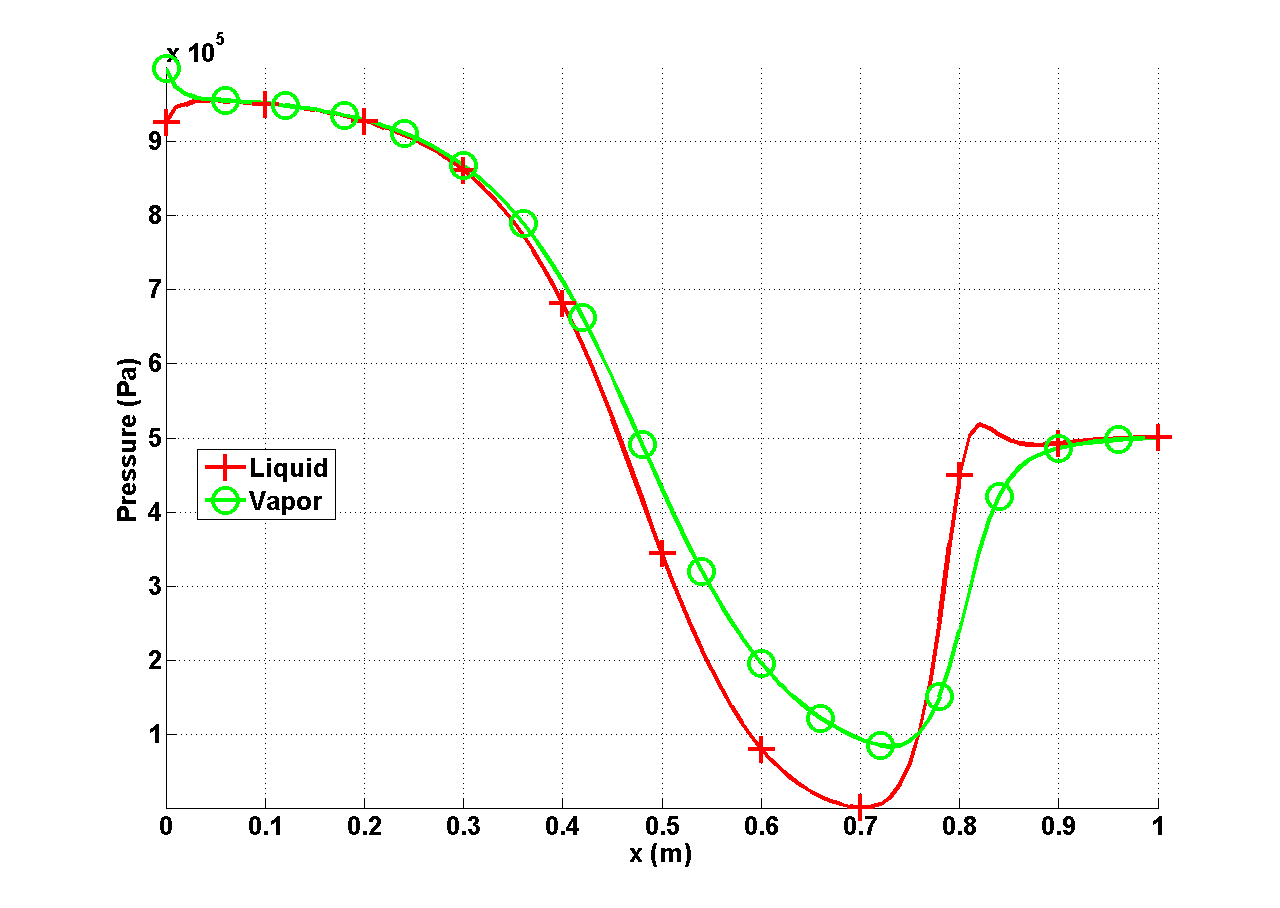
\includegraphics[width=\textwidth]{figures/SEM/Aint1e3_two_phases_pressure.png}
\caption{Pressure profiles at steady state with $A_{int,max} = 10^3$.}
\label{fig:two-fluids-rel-nozzle-press-Aint3-sem-sect4}
\end{figure}
%
\begin{figure}[H]
\centering
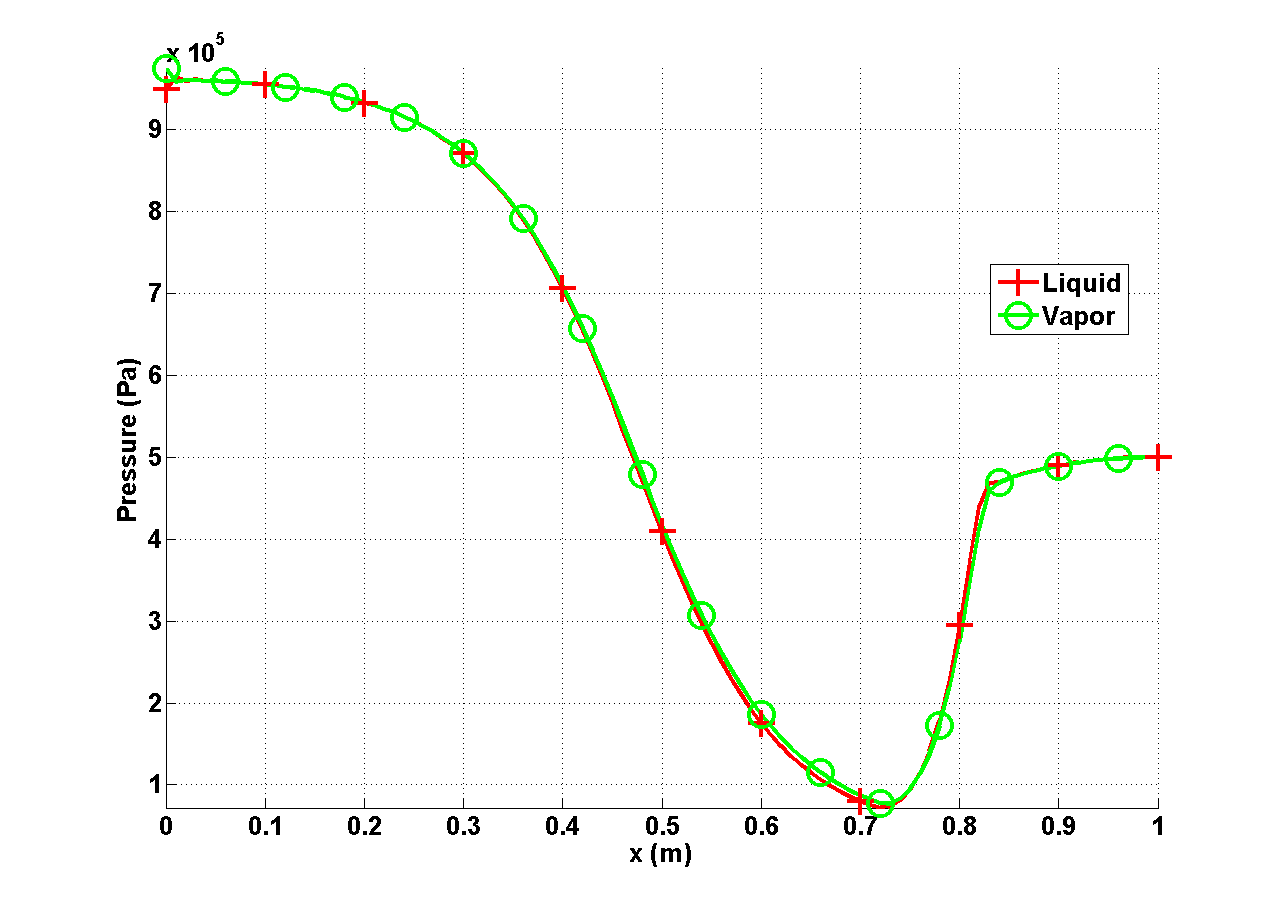
\includegraphics[width=\textwidth]{figures/SEM/Aint1e4_two_phases_pressure.png}
\caption{Pressure profiles at steady state with $A_{int,max} = 10^4$.}
\label{fig:two-fluids-rel-nozzle-press-Aint4-sem-sect4}
\end{figure}
%
The pressure profiles for $A_{int,max} = 10^2 \text{, } 10^3$ and $10^4$ $m^{-1}$ are given in \fig{fig:two-fluids-rel-nozzle-press-Aint2-sem-sect4}, \fig{fig:two-fluids-rel-nozzle-press-Aint3-sem-sect4} and \fig{fig:two-fluids-rel-nozzle-press-Aint4-sem-sect4}, respectively. As the value of $A_{int,max}$ increases, the liquid pressure becomes positive and matches the vapor pressure variations. The static pressure outlet boundary holds for both phases. At the inlet, the liquid and vapor pressures are not equal since the implementation of the boundary condition does not account for the relaxation terms: the static pressure is computed from the stagnation pressure using entropy and enthalpy conservation relations. 
%
\begin{figure}[H]
\centering
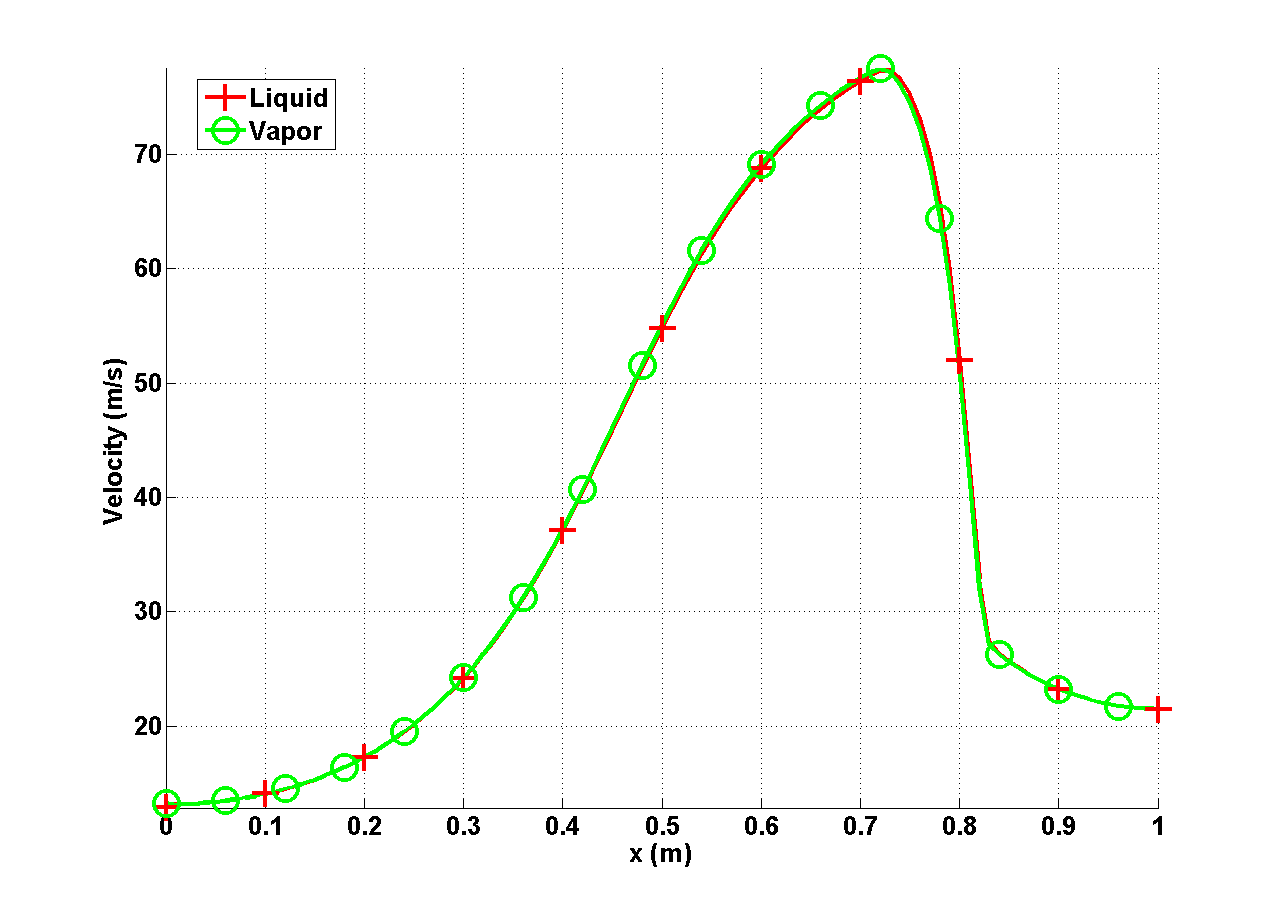
\includegraphics[width=\textwidth]{figures/SEM/Aint1e4_two_phases_velocity.png}
\caption{Velocity profiles at steady state.}
\label{fig:two-fluids-rel-nozzle-vel-sem-sect4}
\end{figure}
%
\begin{figure}[H]
\centering
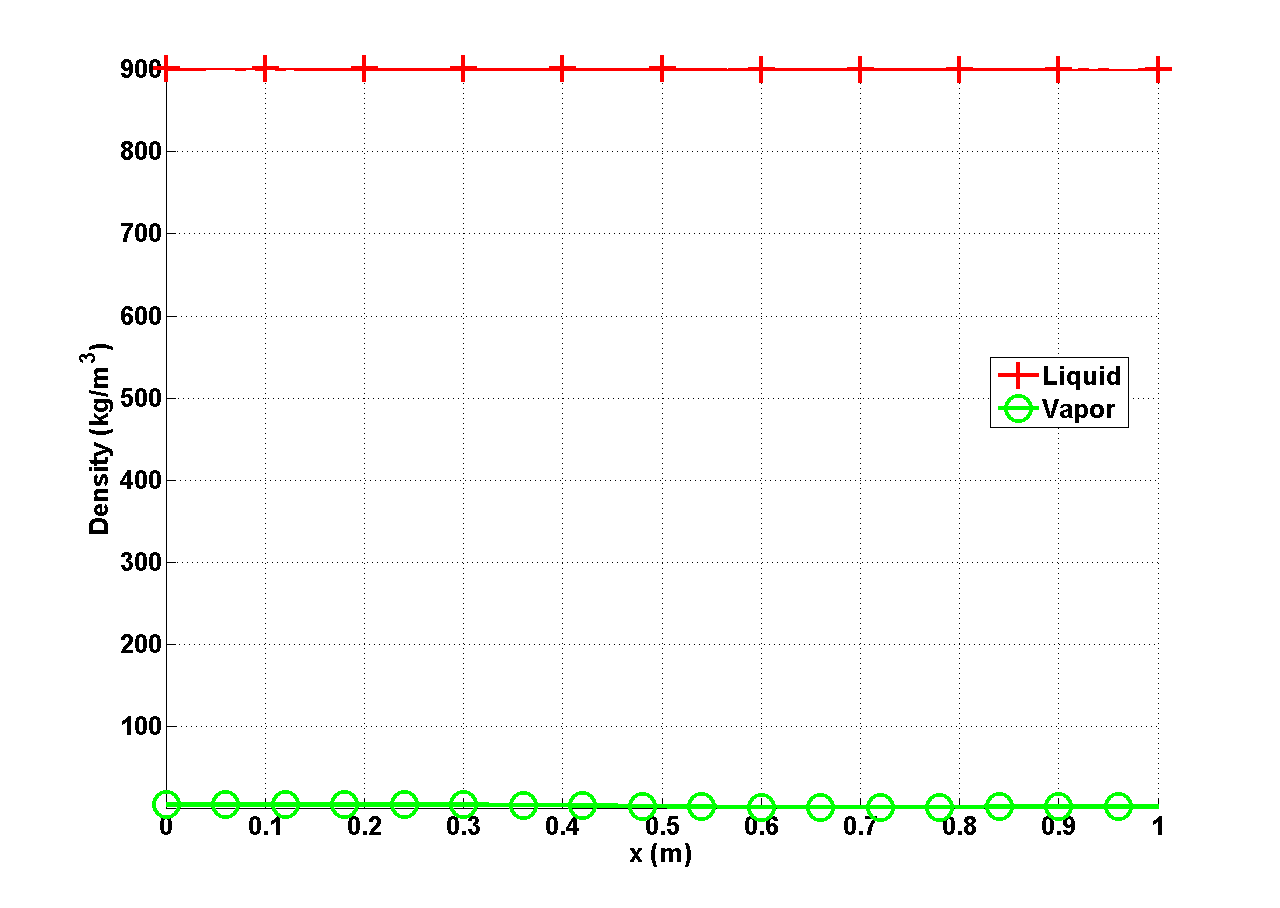
\includegraphics[width=\textwidth]{figures/SEM/Aint1e4_two_phases_density.png}
\caption{Density profiles at steady state.}
\label{fig:two-fluids-rel-nozzle-rho-sem-sect4}
\end{figure}
%
\begin{figure}[H]
\centering
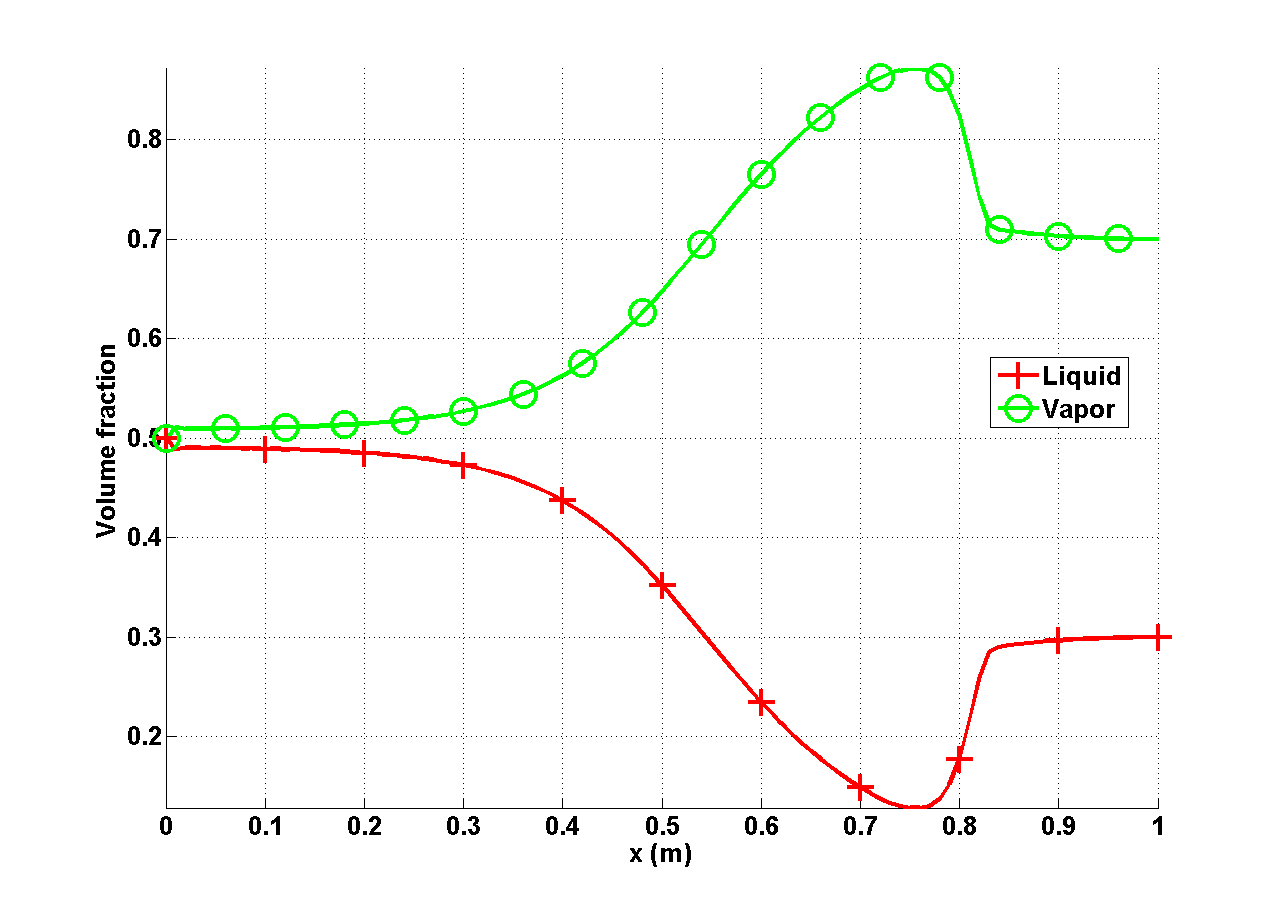
\includegraphics[width=\textwidth]{figures/SEM/Aint1e4_two_phases_volume_fraction.png}
\caption{Volume fraction profiles at steady state.}
\label{fig:two-fluids-rel-nozzle-vf-sem-sect4}
\end{figure}
%
\begin{figure}[H]
\centering
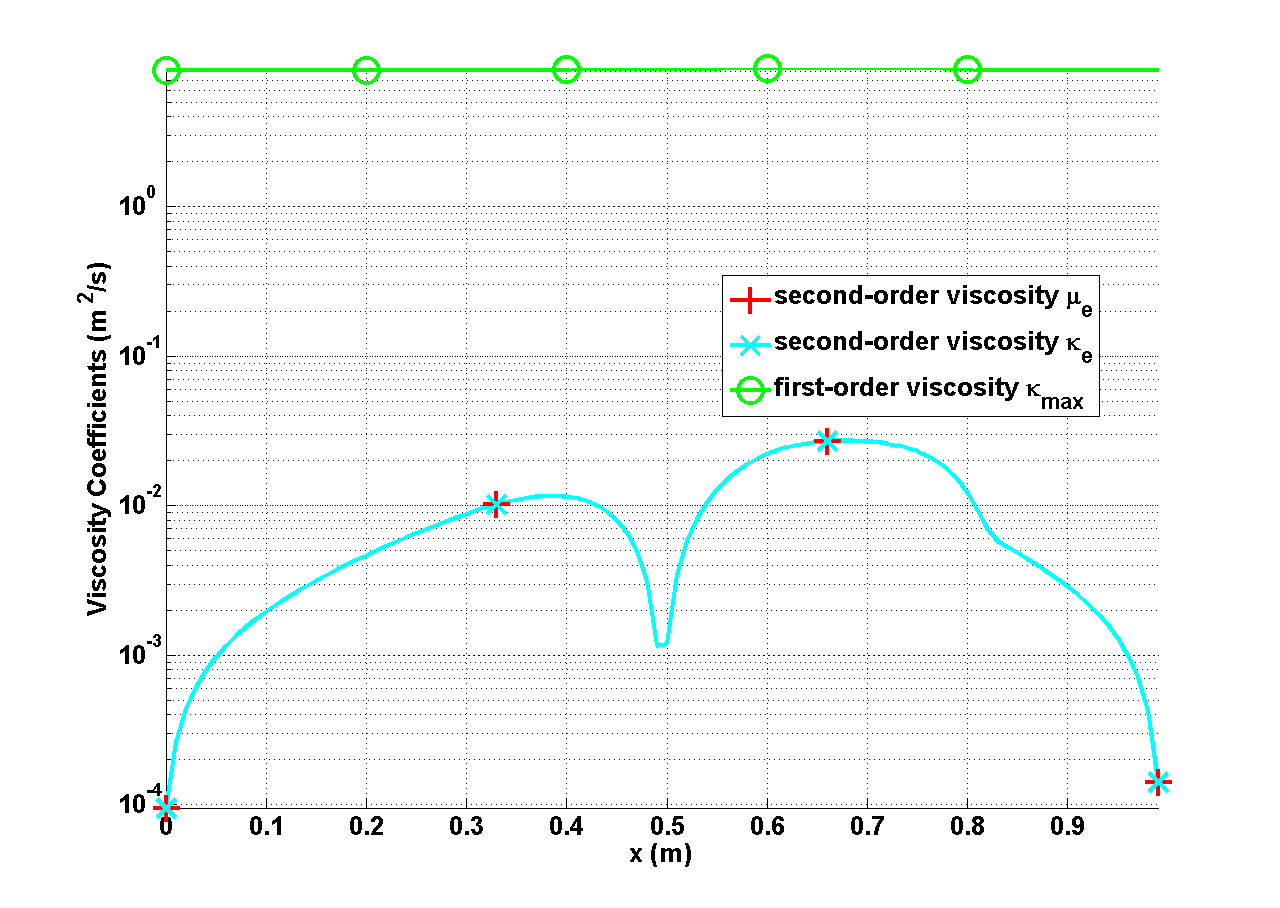
\includegraphics[width=\textwidth]{figures/SEM/Aint1e4_liquid_viscosity_kappa_mu.png}
\caption{Viscosity coefficients profiles for liquid phase at steady state.}
\label{fig:two-fluids-rel-nozzle-visc-liq-sem-sect4}
\end{figure}
%
\begin{figure}[H]
\centering
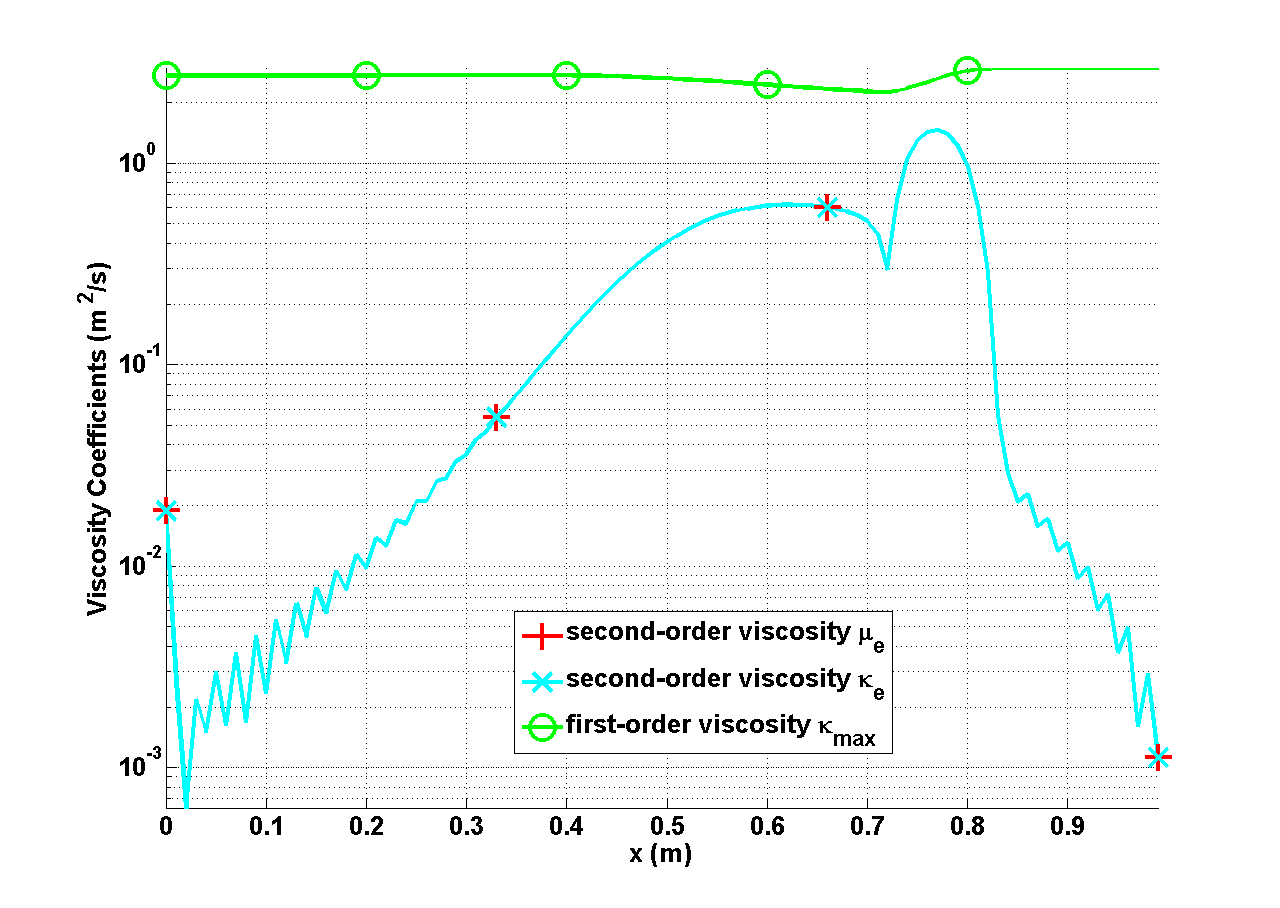
\includegraphics[width=\textwidth]{figures/SEM/Aint1e4_vapor_viscosity_kappa_mu.png}
\caption{Viscosity coefficients profiles for vapor phase at steady state.}
\label{fig:two-fluids-rel-nozzle-visc-vap-sem-sect4}
\end{figure}
%
\begin{figure}[H]
\centering
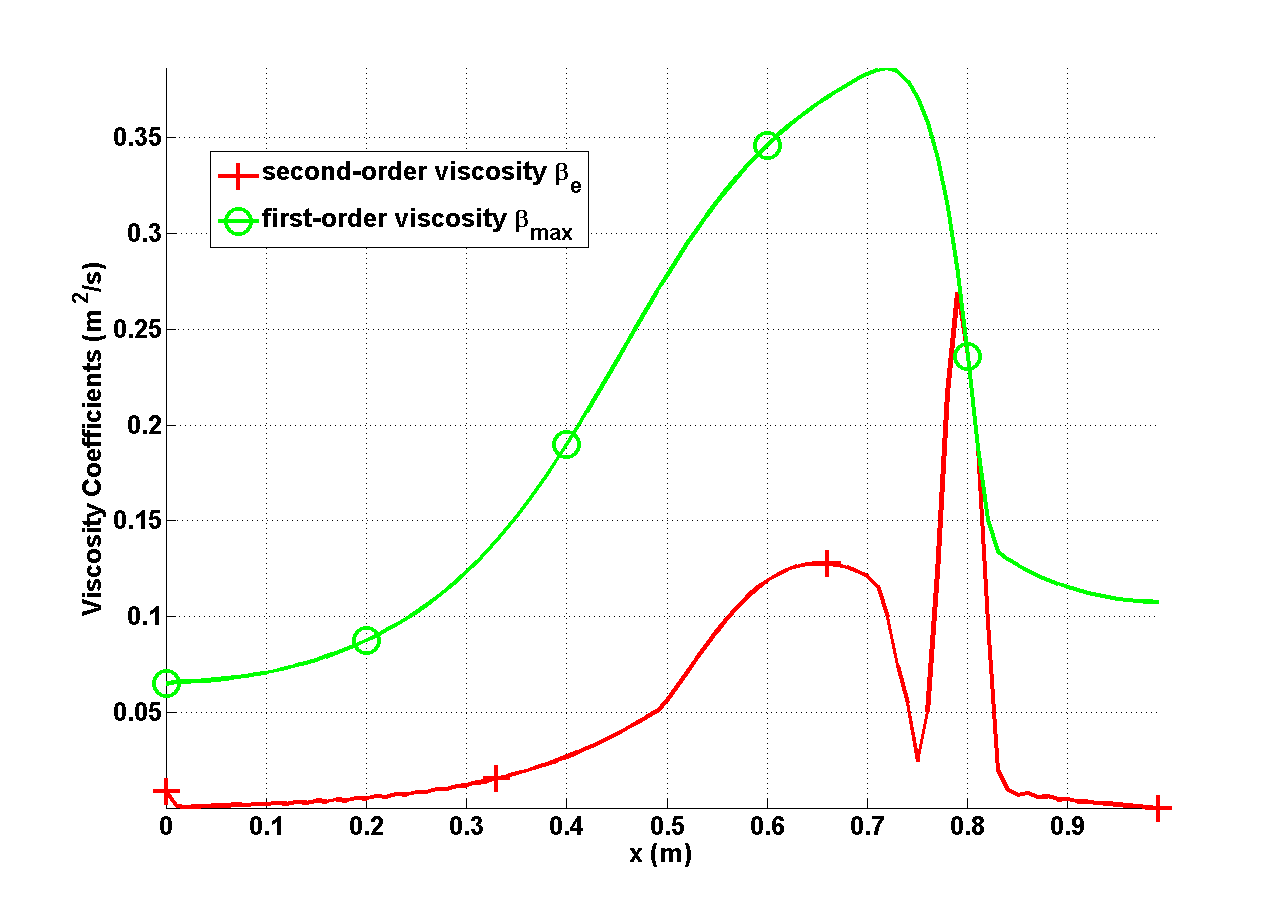
\includegraphics[width=\textwidth]{figures/SEM/Aint1e4_liquid_beta.png}
\caption{Viscosity coefficients profiles for liquid volume fraction phase at steady state.}
\label{fig:two-fluids-rel-nozzle-visc-vf-sem-sect4}
\end{figure}
%
The velocity, density, volume fraction and viscosity coefficients profiles are plotted from \fig{fig:two-fluids-rel-nozzle-vel-sem-sect4} to \ref{fig:two-fluids-rel-nozzle-visc-vf-sem-sect4} in the case $A_{int,max} = 10^4$ $m^{-1}$. Because of the velocity relaxation source terms, velocity equilibrium holds between the liquid and vapor phases. The liquid and vapor density profiles are different by two order of magnitude. The volume fraction of both phases varies throughout the nozzle as a consequence of the pressure equilibrium. The viscosity coefficients $\mu_k$ and $\kappa_k$ are equal to each other since there are no shock waves and are large enough to stabilize the strong variations in the pressure and velocity profiles. Lastly, the viscosity coefficient $\beta_k$ follows the variations of the volume fraction for both phases. It is interesting to note that the fast vapor flow yields strong variations in the divergent part of the nozzle. Overall, the viscosity coefficients are large enough to prevent the formation of any numerical instability without altering the physical solution.

Next, the same converging-diverging nozzle is run with mass and energy exchange source terms. The code is run until steady-state with $A_{int,max}=10^3$ $m^{-1}$. The corresponding numerical results are shown from \fig{fig:two-fluids-rel-nozzle-press-mass-on-sem-sect4} to \ref{fig:two-fluids-rel-nozzle-visc-vf-mass-on-sem-sect4}.
%
\begin{figure}[H]
\centering
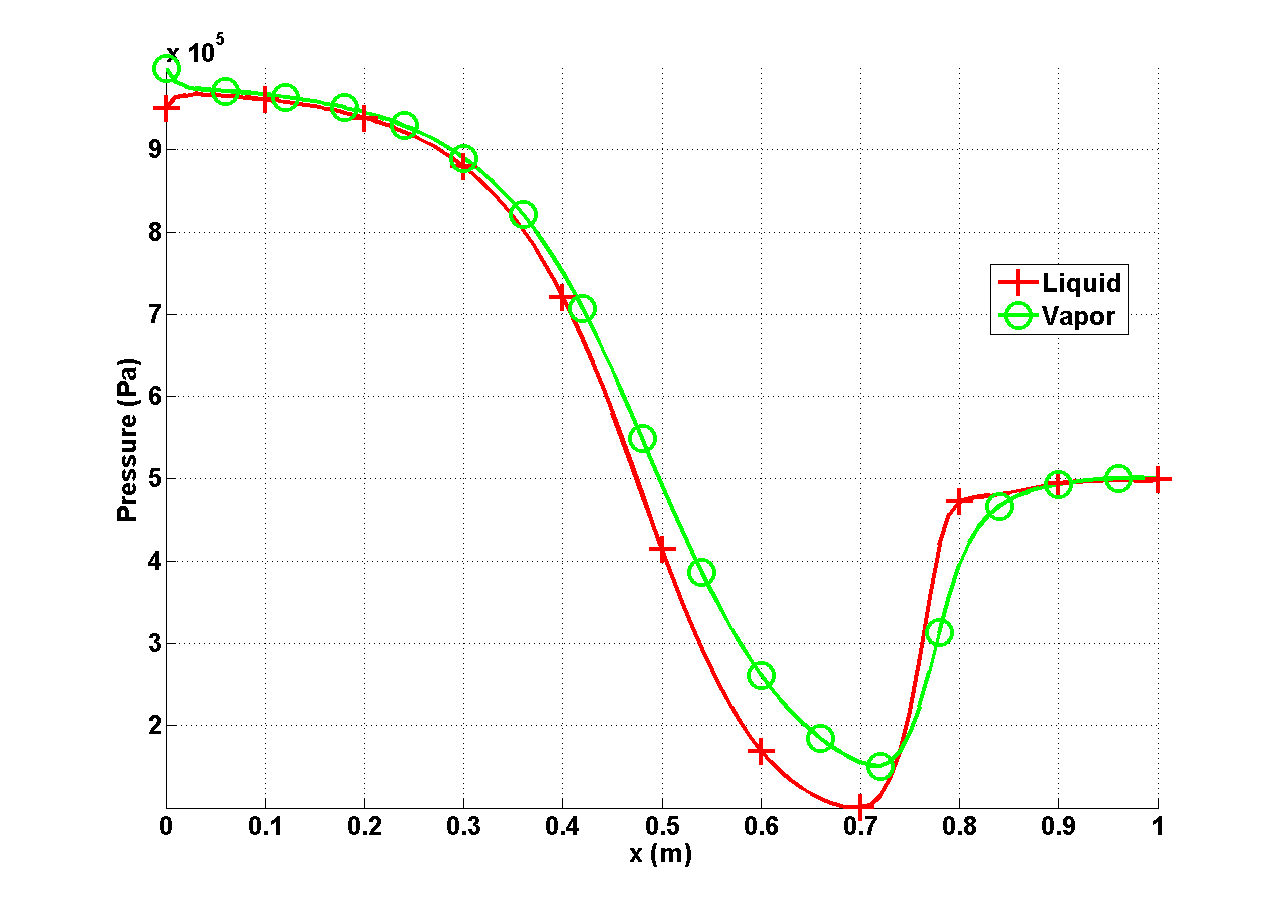
\includegraphics[width=\textwidth]{figures/SEM/Aint1e3MassOn_two_phases_pressure.png}
\caption{Pressure profiles at steady state with thermodynamic relaxations and mass and heat exchange terms.}
\label{fig:two-fluids-rel-nozzle-press-mass-on-sem-sect4}
\end{figure}
%
\begin{figure}[H]
\centering
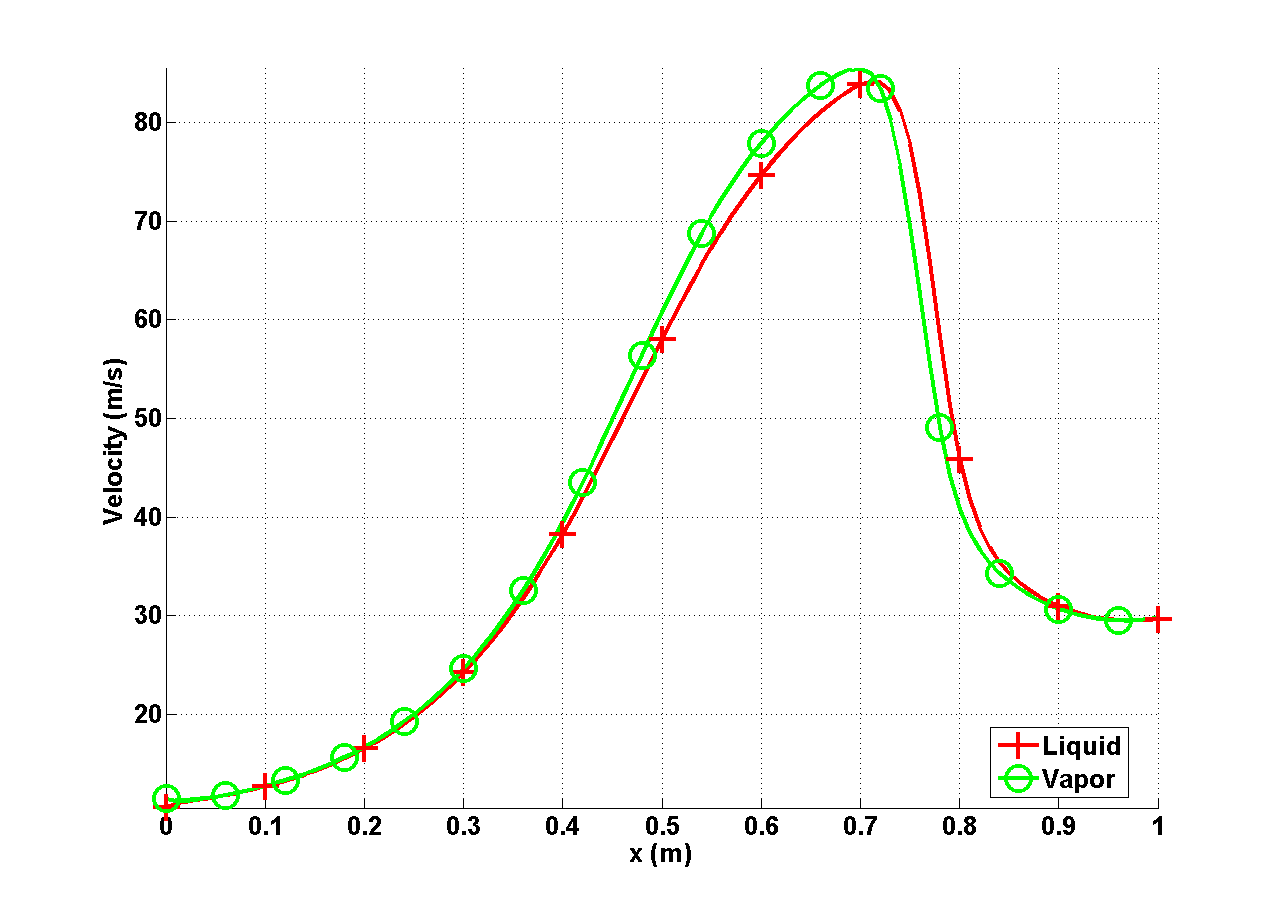
\includegraphics[width=\textwidth]{figures/SEM/Aint1e3MassOn_two_phases_velocity.png}
\caption{Velocity profiles at steady state with thermodynamic relaxations and mass and heat exchange terms.}
\label{fig:two-fluids-rel-nozzle-vel-mass-on-sem-sect4}
\end{figure}
%
\begin{figure}[H]
\centering
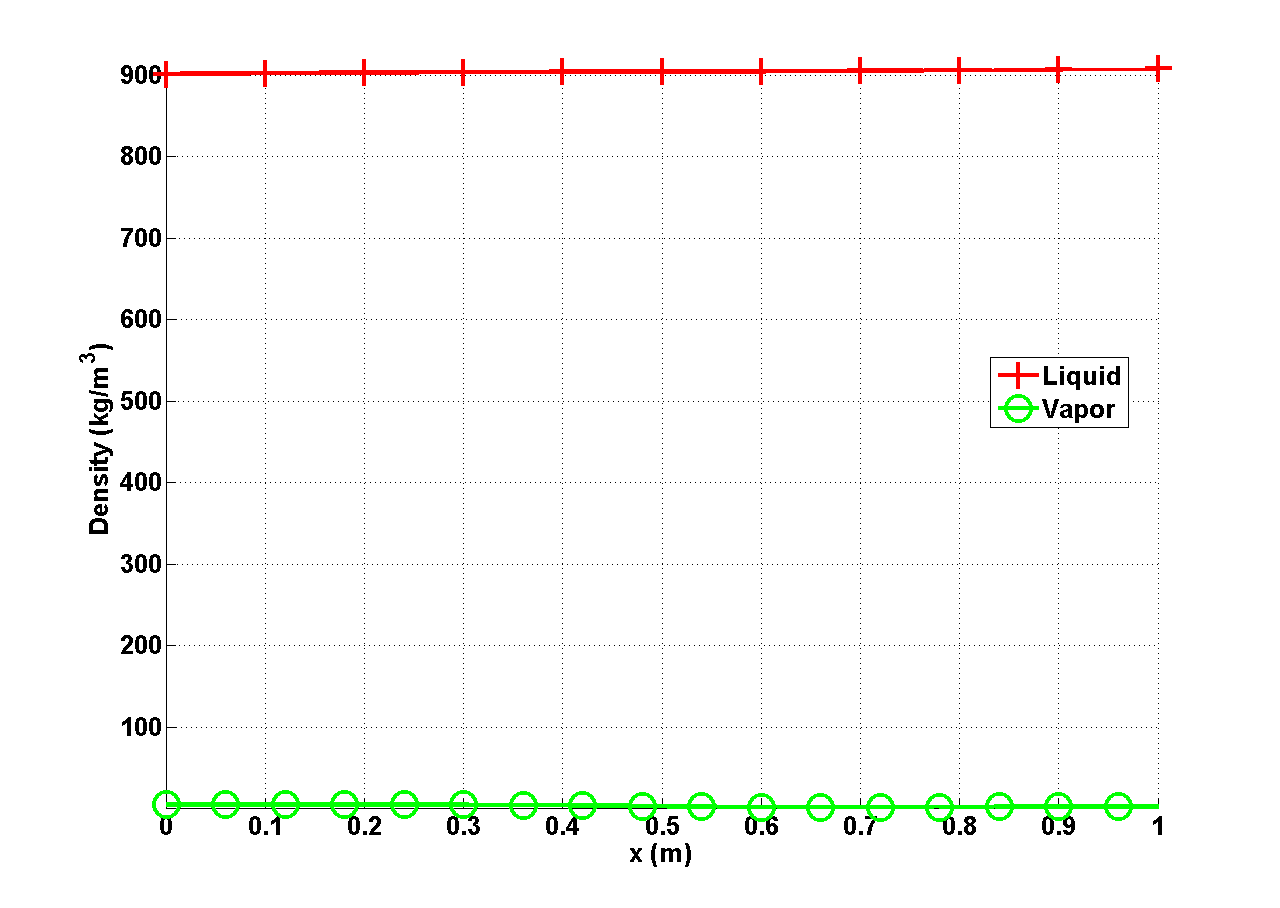
\includegraphics[width=\textwidth]{figures/SEM/Aint1e3MassOn_two_phases_density.png}
\caption{Density profiles at steady state with thermodynamic relaxations and mass and heat exchange terms}
\label{fig:two-fluids-rel-nozzle-rho-mass-on-sem-sect4}
\end{figure}
%
\begin{figure}[H]
\centering
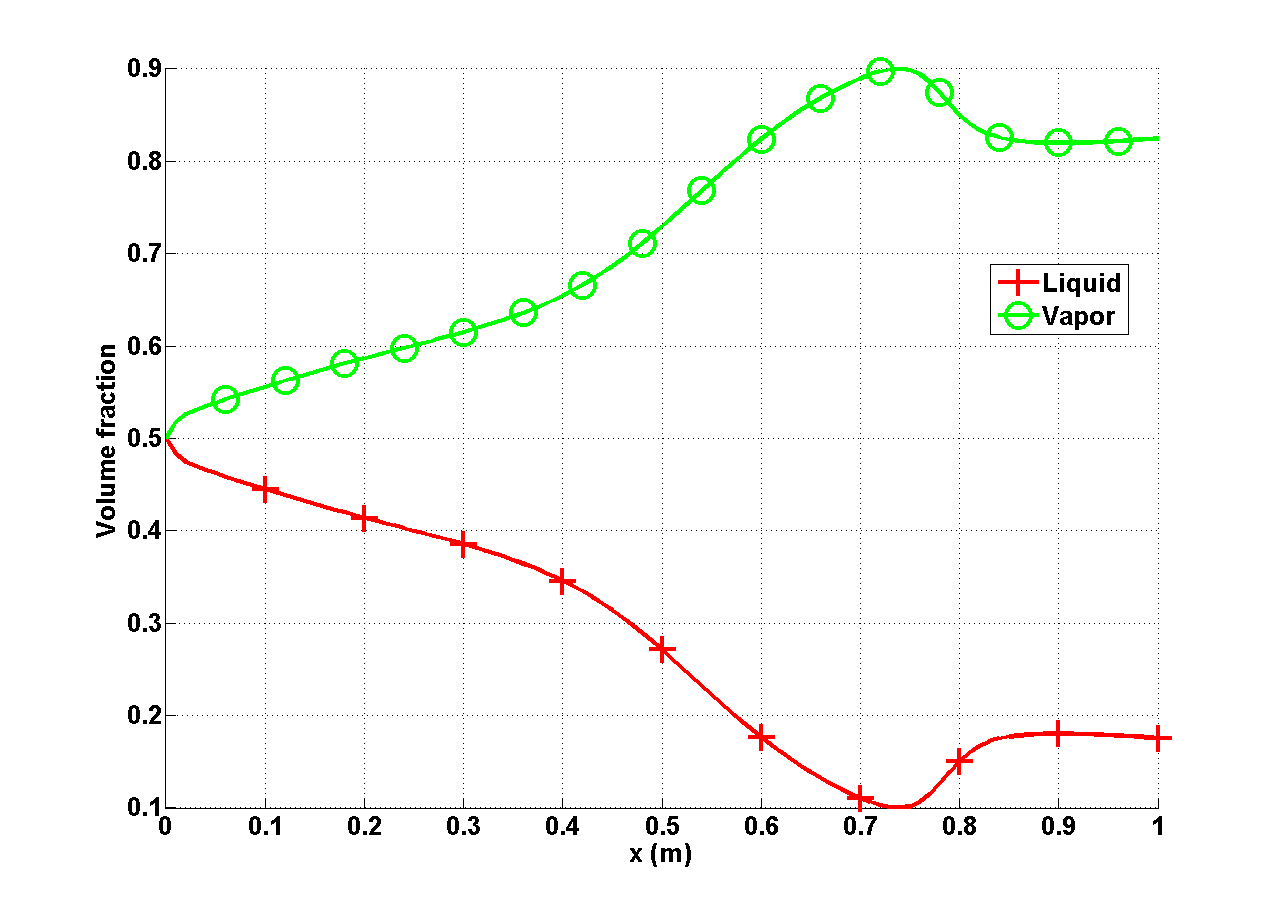
\includegraphics[width=\textwidth]{figures/SEM/Aint1e3MassOn_two_phases_volume_fraction.png}
\caption{Volume fraction profiles at steady state with thermodynamic relaxations and mass and heat exchange terms.}
\label{fig:two-fluids-rel-nozzle-vf-mass-on-sem-sect4}
\end{figure}
%
\begin{figure}[H]
\centering
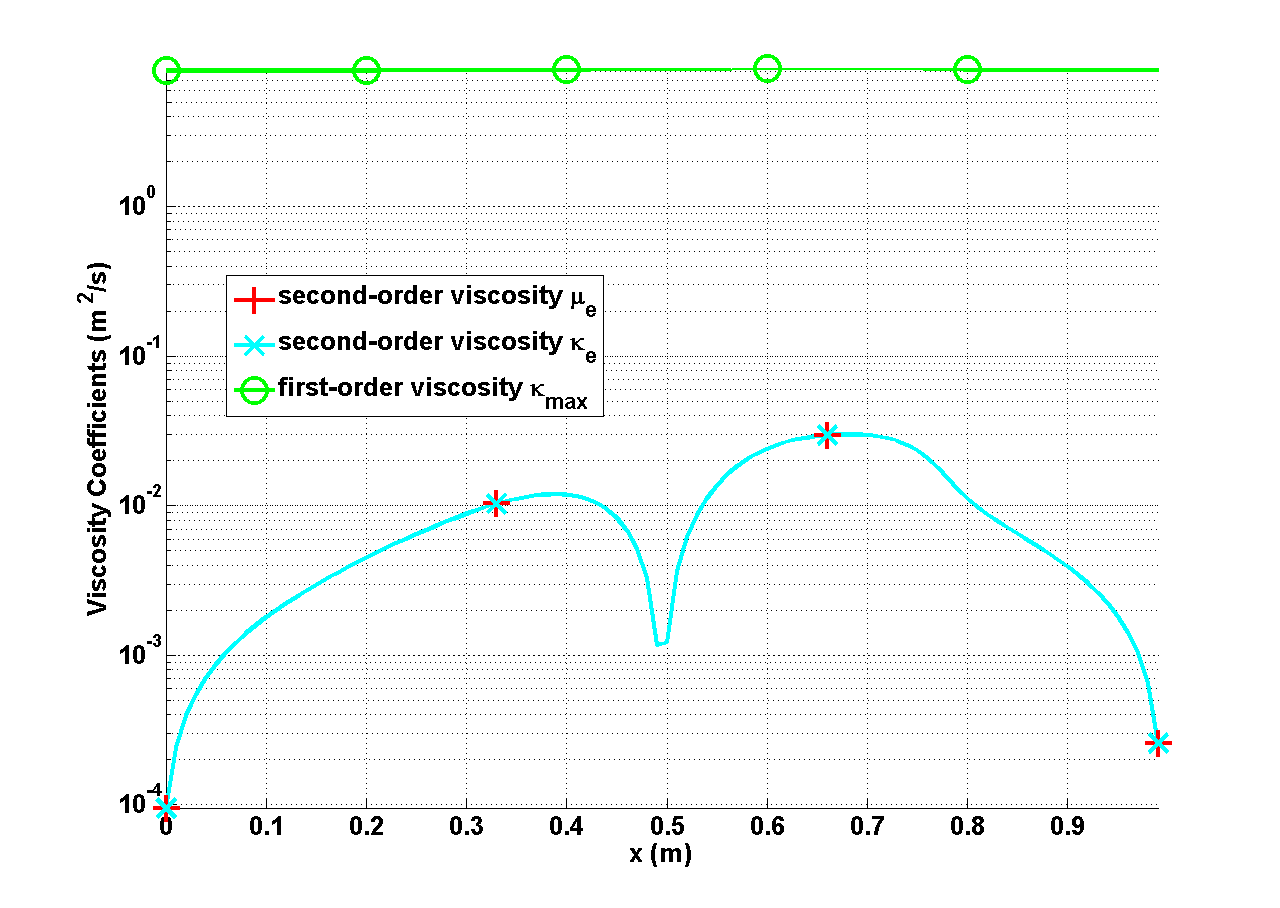
\includegraphics[width=\textwidth]{figures/SEM/Aint1e3MassOn_liquid_viscosity_kappa_mu.png}
\caption{Viscosity coefficients profiles for liquid phase at steady state with thermodynamic relaxations and mass and heat exchange terms.}
\label{fig:two-fluids-rel-nozzle-visc-liq-mass-on-sem-sect4}
\end{figure}
%
\begin{figure}[H]
\centering
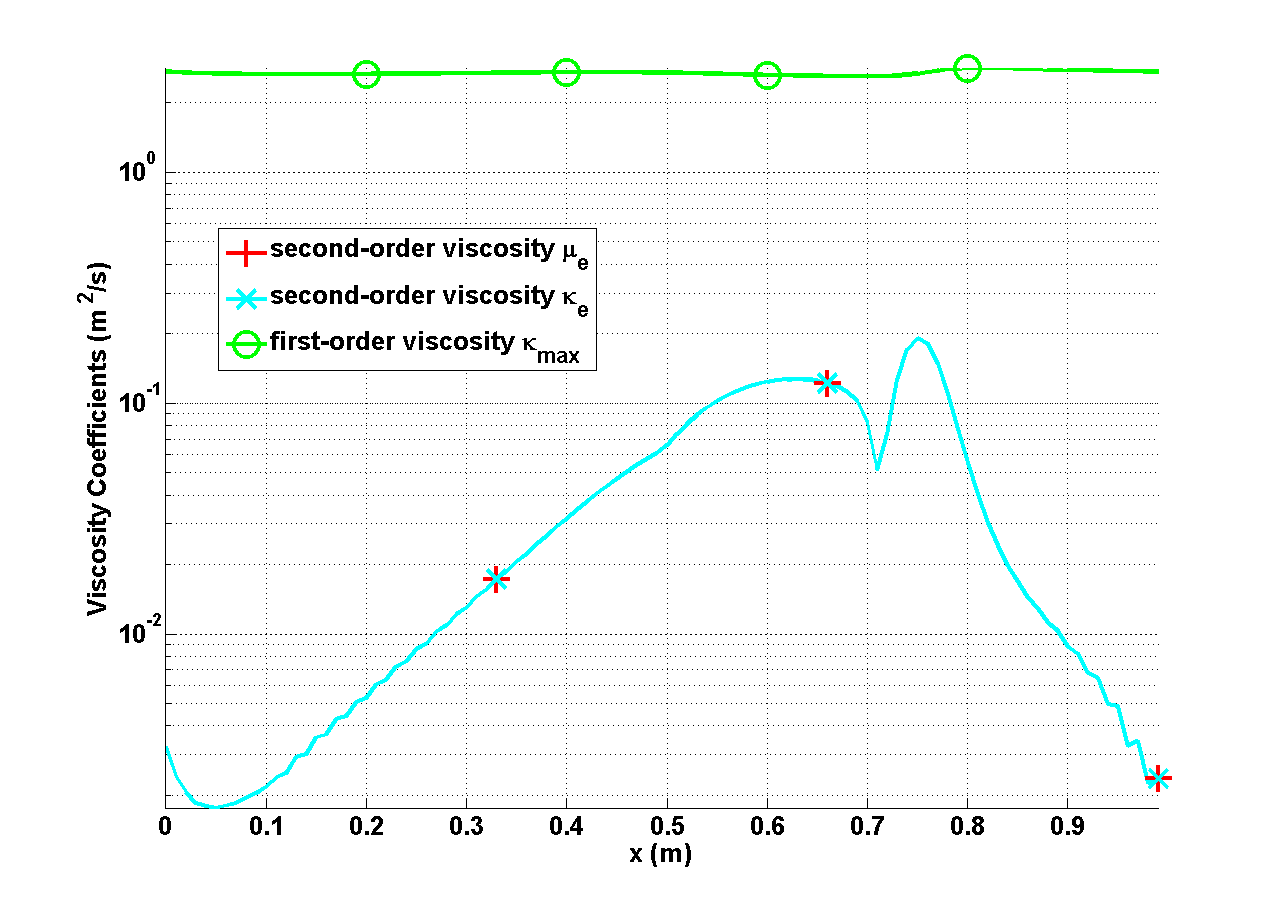
\includegraphics[width=\textwidth]{figures/SEM/Aint1e3MassOn_vapor_viscosity_kappa_mu.png}
\caption{Viscosity coefficients profiles for vapor phase at steady state with thermodynamic relaxations and mass and heat exchange terms.}
\label{fig:two-fluids-rel-nozzle-visc-vap-mass-on-sem-sect4}
\end{figure}
%
\begin{figure}[H]
\centering
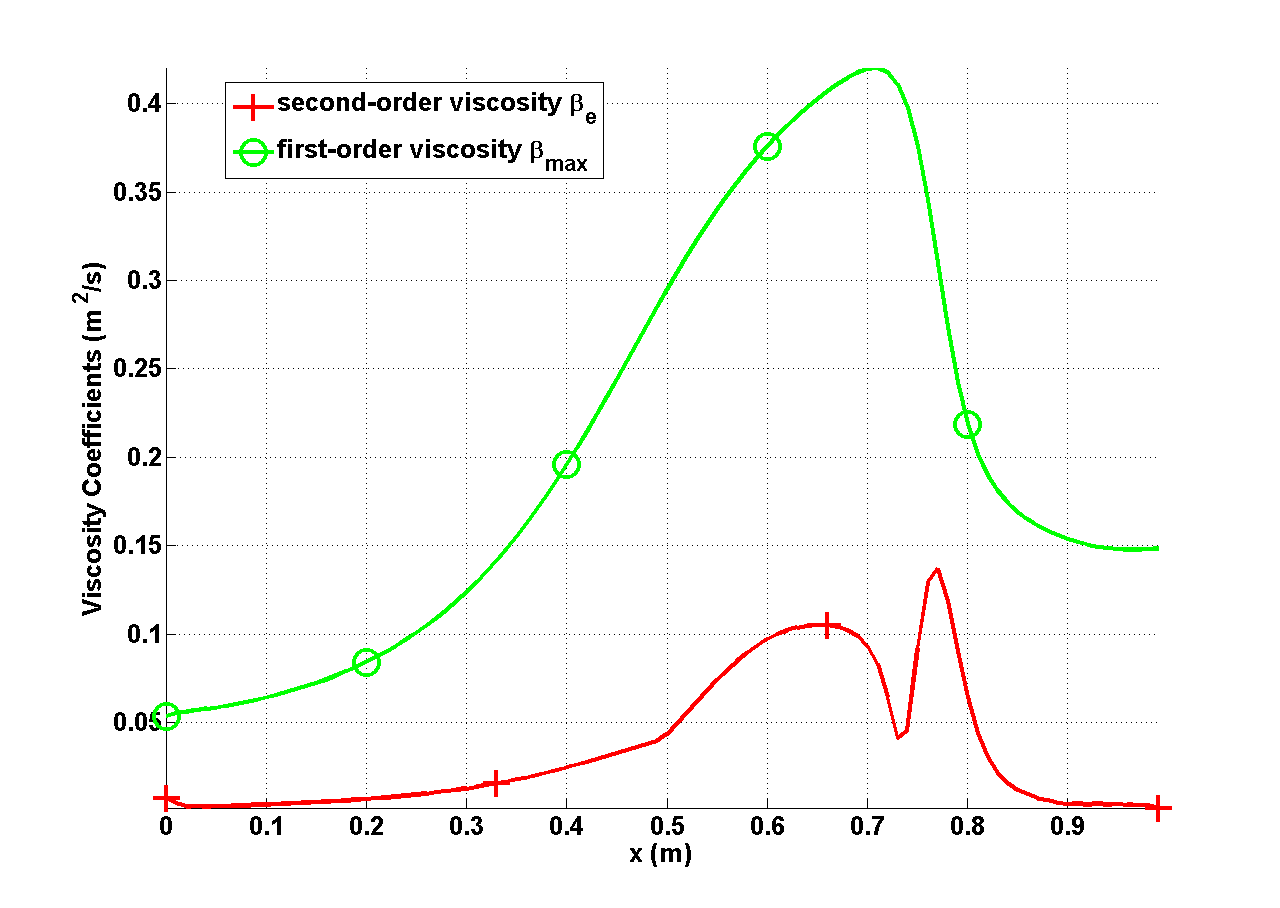
\includegraphics[width=\textwidth]{figures/SEM/Aint1e3MassOn_liquid_beta.png}
\caption{Viscosity coefficients profiles for liquid volume fraction at steady state with thermodynamic relaxations and mass and heat exchange terms.}
\label{fig:two-fluids-rel-nozzle-visc-vf-mass-on-sem-sect4}
\end{figure}
%
Because of the mass and heat transfers between phases, the flow variations are smoother than in the previous case. Consequently, the viscosity coefficients are also smoother while effectively stabilizing the scheme.  
%-------------------------------------------------------------------------------------------------------------------------------------------------
\subsection{1-D straight pipe with wall-friction force, wall heat source and exchange terms (mass and energy)}\label{sec:1d-straight-pipe-7-eq-sct4}
%-------------------------------------------------------------------------------------------------------------------------------------------------
We present one sample result for a 1-D straight pipe of constant area $A = 10^{-4}$ $m^2$ with a wall heat source (the wall temperature is constant: $T_w = 550$ $K$). The stiffened gas equation of state is used to model the liquid and vapor phases with the parameters taken from \cite{SGEOS} for each phase. A static pressure of $P=7.1$ $MPa$ is set at the outlet. The volume fraction, the enthalpy and the mass flow rate are specified at the inlet for each phase. The wall friction coefficient is constant and the same for the two phases, $f_w = 4 \times 10^{-2}$. The interfacial area $A_{int}$ is set to a large value to equalize the pressure and velocity of the two phases. The initial conditions are uniform. The geometry is discretized with a uniform mesh of 100 elements and the simulation is run with CFL$=100$  until a steady state is obtained. 

The pressure, temperature, velocity, volume fraction and viscosity coefficients profiles are plotted from \fig{fig:pressure} through \fig{fig:viscosity_coeff}. As expected, the liquid and vapor pressure profiles are identical (\fig{fig:pressure}) and decrease throughout the domain because of wall friction. The liquid and velocity profiles are also identical as shown in \fig{fig:velocity} and increase due to the wall friction force and the heat addition. In \fig{fig:temperature}, the liquid and vapor temperature profiles are distinct and have the same variation: the temperature rises since energy is added to the flow by the wall heat source. The variations of the vapor and liquid volume fractions are opposite: vapor is produced since the liquid temperature is larger than the saturation temperature. All of the profiles are smooth and do not display any spurious oscillations: the entropy viscosity coefficients shown in \fig{fig:viscosity_coeff}, $\kappa_{e,k}$ and $\beta_{e,k}$, are well-scaled and large enough to stabilize the numerical solution without altering it (only $\beta_{e,liquid}$ is plotted since $\beta_{e,liquid}=\beta_{e,vapor}$). It is also noted the difference of several order of magnitude between the entropy viscosity and first-order viscosity coefficients denoted by the subscript $max$. The first-order viscosity coefficients are over-dissipative and ill-scaled in the low Mach regime.
%
        \begin{figure}[H]
                \centering
                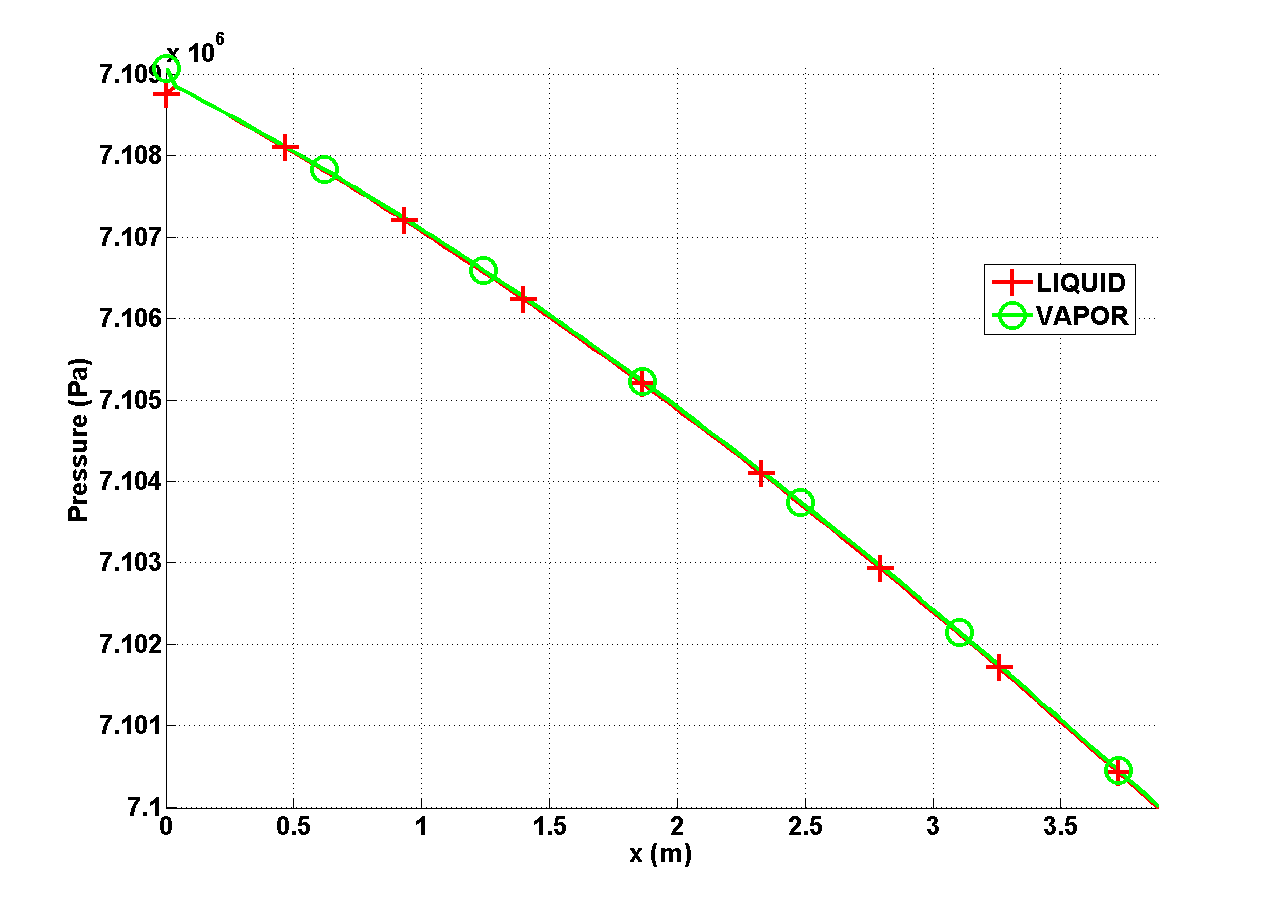
\includegraphics[width=\textwidth]{figures/SEM/ANS_WINTER_2014_7Eqn_pressure.png}
                \caption{Pressure profiles at steady-state}
                \label{fig:pressure}
        \end{figure}%
%
        \begin{figure}[H]
                \centering
                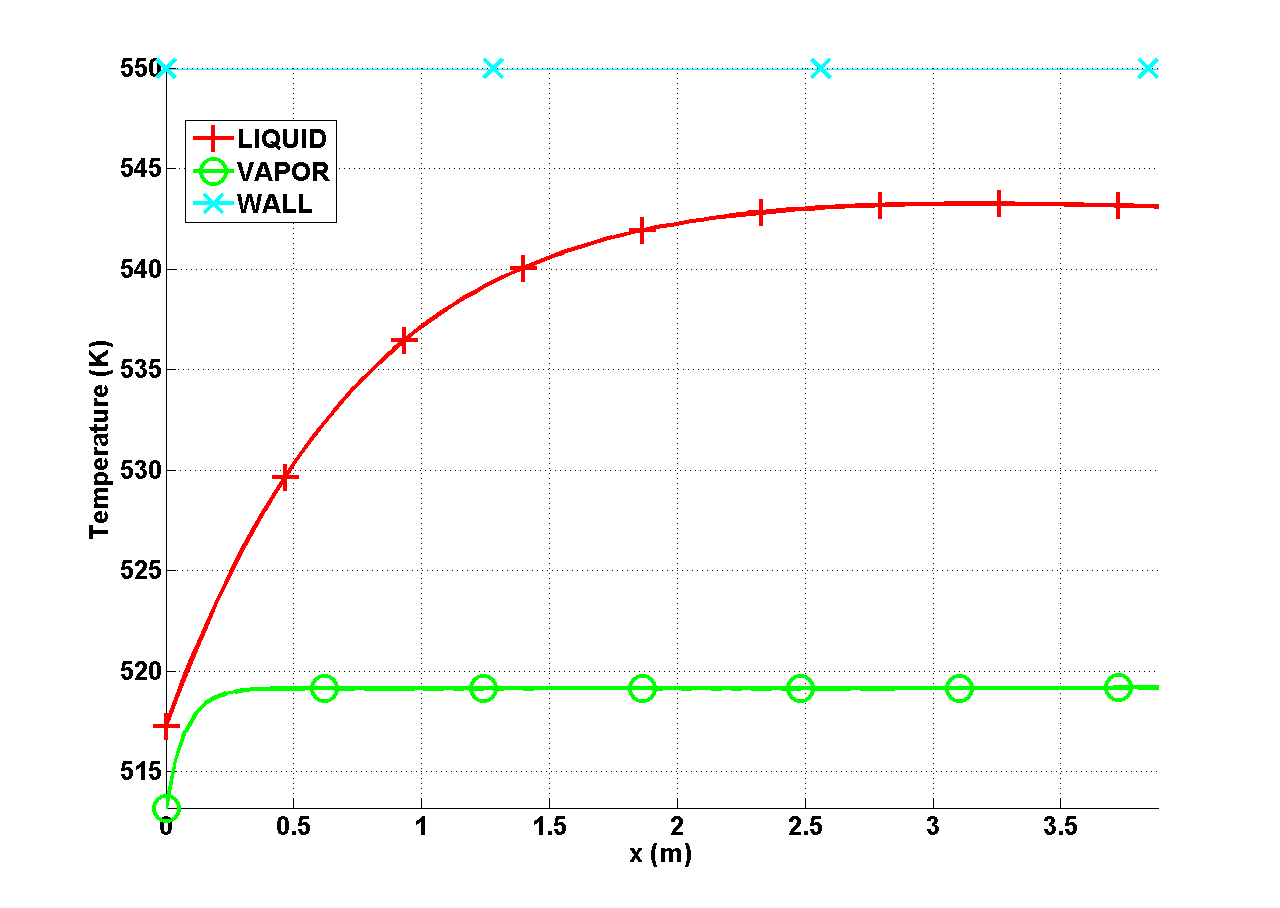
\includegraphics[width=\textwidth]{figures/SEM/ANS_WINTER_2014_7Eqn_temperature.png}
                \caption{Temperature profiles at steady-state}
                \label{fig:temperature}
        \end{figure}%
%            
        \begin{figure}[H]
                \centering
                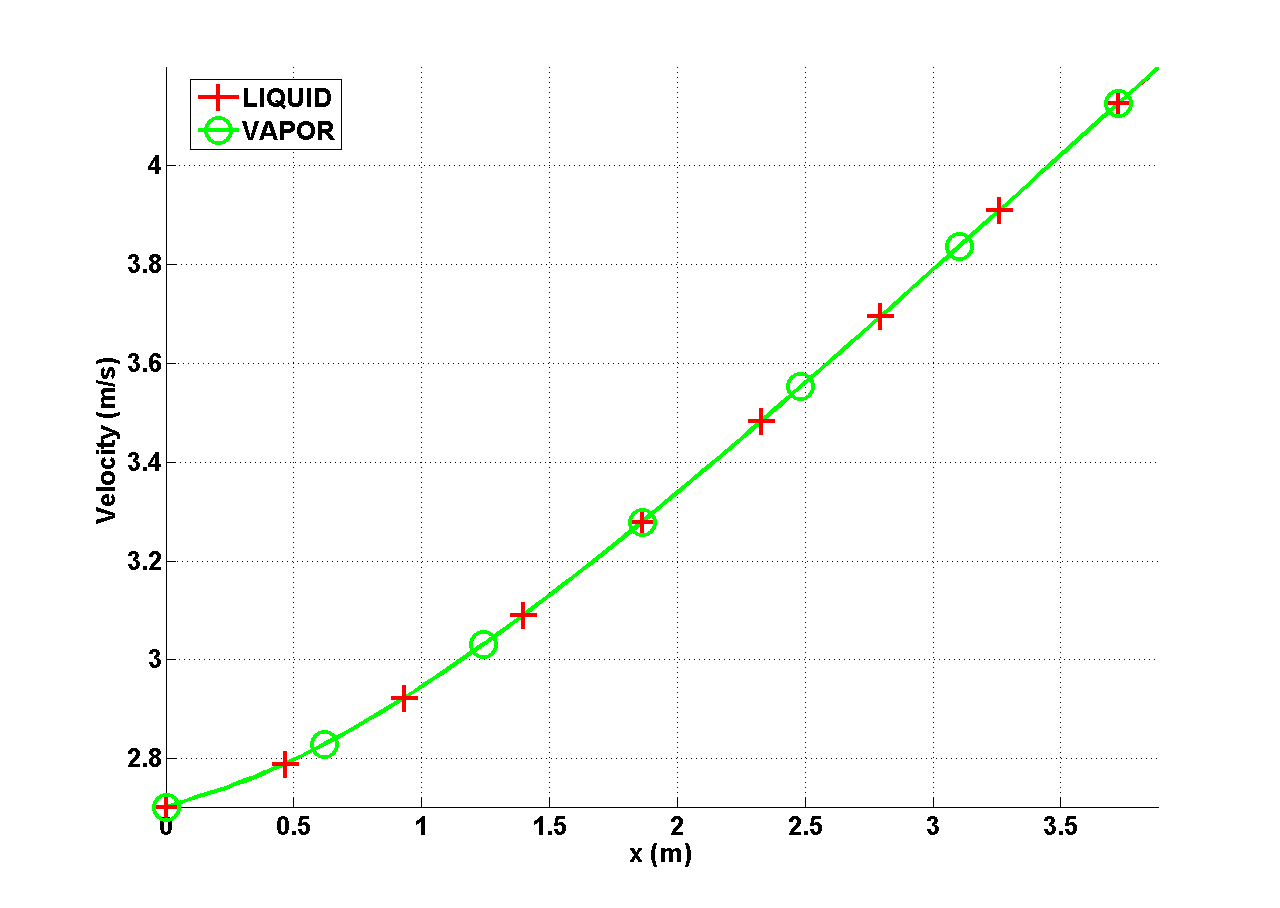
\includegraphics[width=\textwidth]{figures/SEM/ANS_WINTER_2014_7Eqn_velocity.png}
                \caption{Velocity profiles at steady-state}
                \label{fig:velocity}
        \end{figure}
%
        \begin{figure}[H]
                \centering
                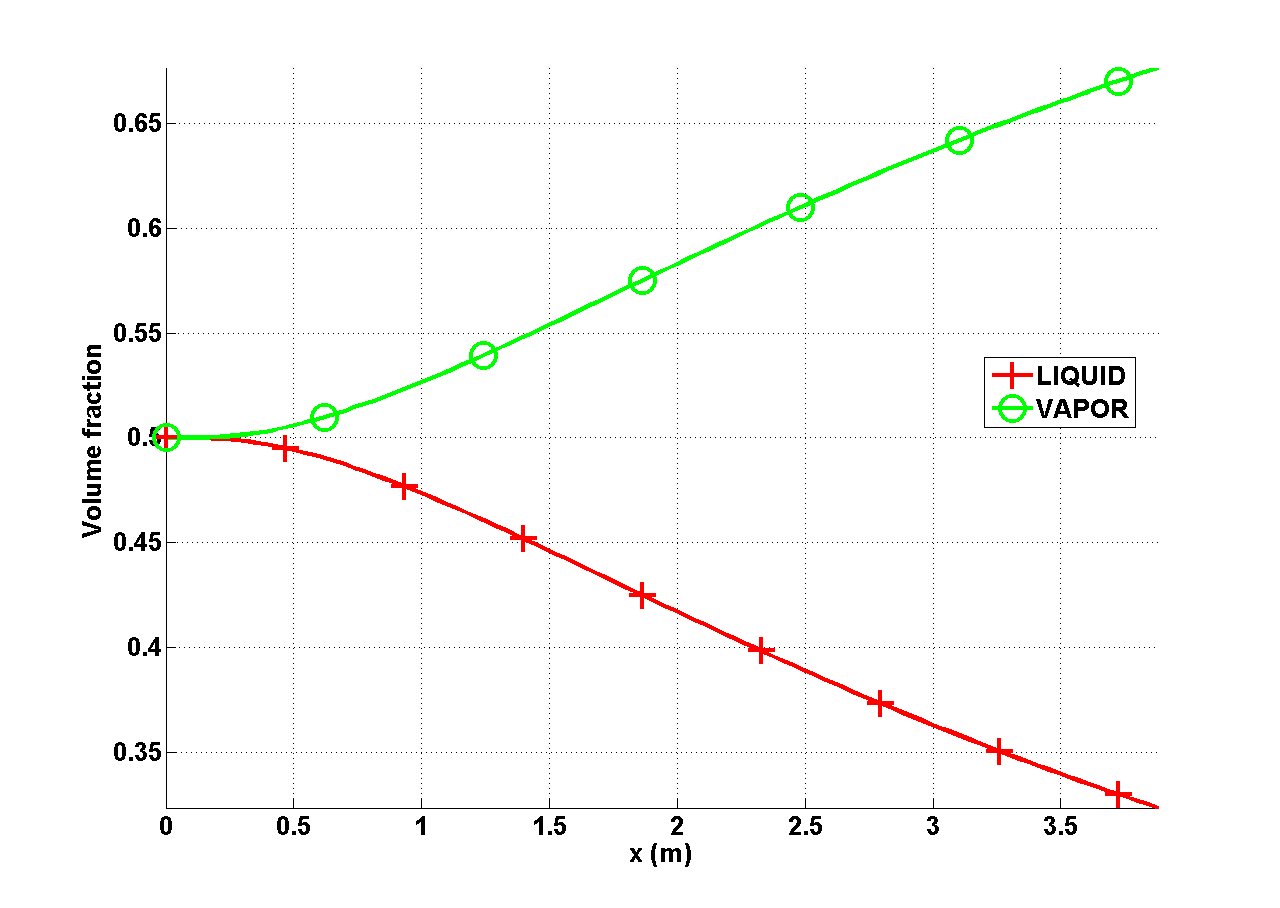
\includegraphics[width=\textwidth]{figures/SEM/ANS_WINTER_2014_7Eqn_volume_fraction.png}
                \caption{Volume fraction profiles at steady-state}
                \label{fig:volume_fraction}
        \end{figure}        
%
        \begin{figure}[H]
                \centering
                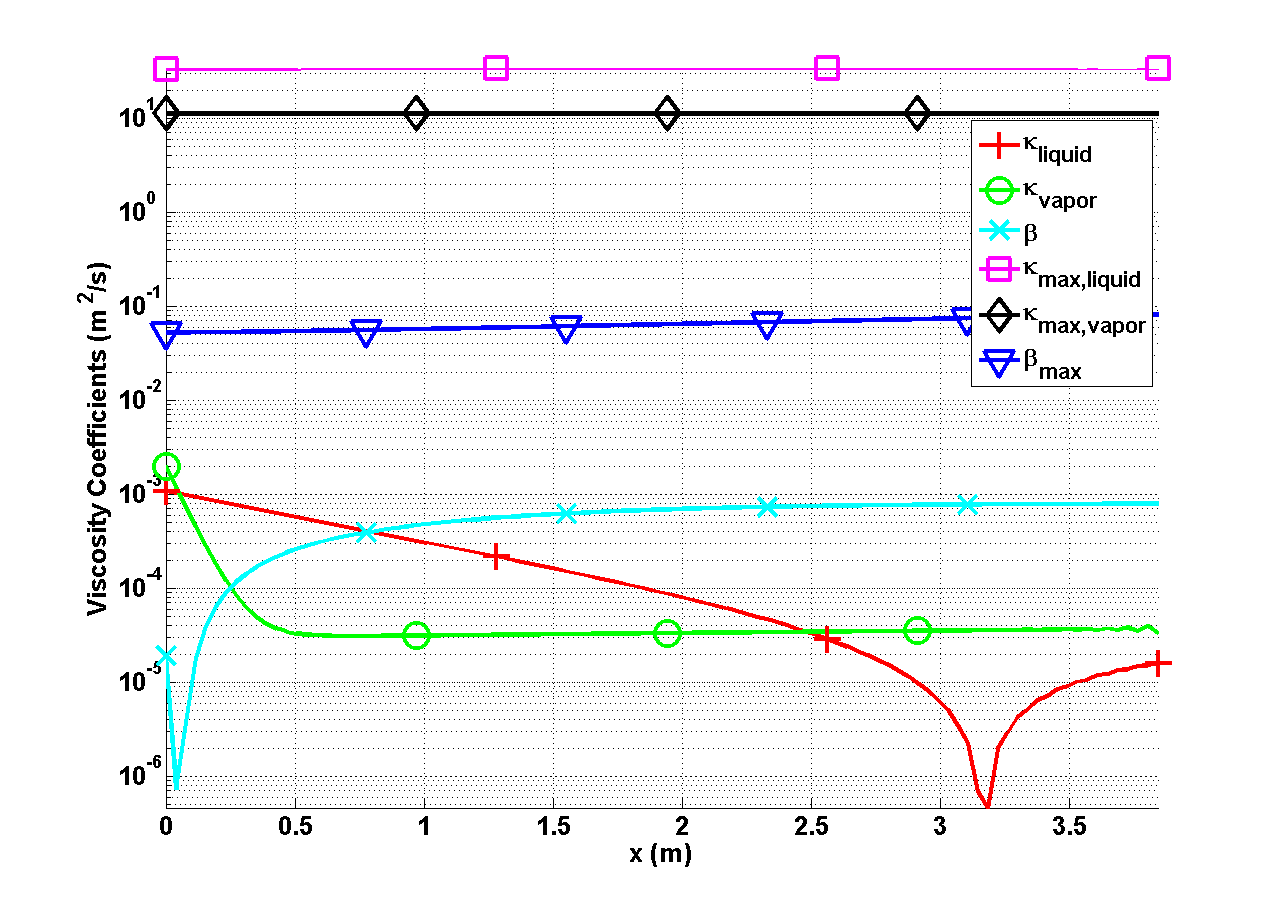
\includegraphics[width=\textwidth]{figures/SEM/ANS_WINTER_2014_7Eqn_viscosity.png}
                \caption{Viscosity coefficients profiles at steady-state}
                \label{fig:viscosity_coeff}
        \end{figure}        
%
%Because it is not economical to solve the entire two-phase flow field
%with highly resolved three-dimensional computational fluid dynamics for an
%entire light water reactor coolant system,
%it is necessary to construct a one-dimensional model for flow in
%pipes, nozzles, and other components.  The one-dimensional model is
%constructed to allow the representation of continuously variable
%cross-sectional area.
%
%Consider flow through a duct with local cross-sectional area
%$A=A(x,t)$.  Actually, most of the time we consider local
%cross-sectional area to depend upon position coordinate $x$ only,
%for which a time rate of change of cross-sectional area is not
%necessary because for this case $\frac{\partial A}{\partial
%t} = 0$.  However, $A(x,t)$ is left inside the time derivative terms
%for generality and possible future use.  The seven-equation two-phase
%system model can be stated as balances of mass, momentum, and total energy,
%along with volume fraction evolution as
%\begin{align}
%  % liquid mass conservation
%  \label{E-R:74}
%  \frac{\partial \left( \alpha \rho \right)_{liq} A}{\partial t}
%  + \frac{\partial \left( \alpha \rho u \right)_{liq} A}{\partial x}
%  &= - \Gamma A_{int} A
%  \\
%  % liquid momentum
%  \nonumber
%  \frac{\partial \left( \alpha \rho u \right)_{liq} A}{\partial t}
%  + \frac{\partial \alpha_{liq} A \left( \rho u^2 + p \right)_{liq} }{\partial x}
%  &= P_{int} A \frac{\partial \alpha_{liq}}{\partial x} + p_{liq} \alpha_{liq} \frac{\partial A}{\partial x}
%  \\
%  \nonumber
%  &+ A \lambda_u (u_{vap} - u_{liq})
%  \\
%  \nonumber
%  &- \Gamma A_{int} u_{int} A
%  \\
%  \nonumber
%  &- F_{\text{wall friction}, liq} - F_{\text{friction}, vap}
%  \\
%  &+ \left( \alpha \rho \right)_{liq} A \vec{g} \cdot \vec{n}_{axis}
%\end{align}
%\begin{align}
%  % liquid total energy
%  \nonumber
%  \frac{\partial \left( \alpha \rho E \right)_{liq} A}{\partial t}
%  + \frac{\partial \alpha_{liq} u_{liq} A \left( \rho E + p \right)_{liq}}{\partial x}
%  &= P_{int} u_{int} A \frac{\partial \alpha_{liq}}{\partial x} - \bar{P}_{int} A \mu_P (p_{liq} - p_{vap})
%  \\
%  \nonumber
%  &+ \bar{u}_{int} A \lambda_u (u_{vap} - u_{liq})
%  \\
%  \nonumber
%  &+ \Gamma A_{int} \left( \frac{P_{int}}{\rho_{int}} - H_{liq, int} \right) A
%  \\
%  &+ Q_{int, liq} + Q_{\text{wall}, liq}
%  \\
%  % liquid volume fraction
%  \label{eqn:7eqn_va_alpha_liq}
%  \frac{\partial \alpha_{liq} A}{\partial t} + u_{int} A \frac{\partial \alpha_{liq}}{\partial x}
%  &= A \mu_P (p_{liq} - p_{vap}) - \frac{\Gamma A_{int} A}{\rho_{int}}
%\end{align}
%for the liquid phase, and
%\begin{align}
%  % vapor mass conservation
%  \frac{\partial \left( \alpha \rho \right)_{vap} A}{\partial t}
%  + \frac{\partial \left( \alpha \rho u \right)_{vap} A}{\partial x}
%  &=  \Gamma A_{int} A
%  \\
%  % vapor momentum
%  \nonumber
%  \frac{\partial \left( \alpha \rho u \right)_{vap} A}{\partial t}
%  + \frac{\partial \alpha_{vap} A \left( \rho u^2 + p \right)_{vap} }{\partial x}
%  &= P_{int} A \frac{\partial \alpha_{vap}}{\partial x} + p_{vap} \alpha_{vap} \frac{\partial A}{\partial x}
%  \\
%  \nonumber
%  &+ A \lambda_u (u_{liq} - u_{vap})
%  \\
%  \nonumber
%  &+ \Gamma A_{int} u_{int} A
%  \\
%  \nonumber
%  &- F_{\text{wall friction}, vap} - F_{\text{friction}, liq}
%  \\
%  &+ \left( \alpha \rho \right)_{vap} A \vec{g} \cdot \vec{n}_{axis}
%\end{align}
%\begin{align}
%  \nonumber
%  % vapor total energy
%  \frac{\partial \left( \alpha \rho E \right)_{vap} A}{\partial t}
%  + \frac{\partial \alpha_{vap} u_{vap} A \left( \rho E + p \right)_{vap}}{\partial x}
%  &= P_{int} u_{int} A \frac{\partial \alpha_{vap}}{\partial x} - \bar{P}_{int} A \mu_P (p_{vap} - p_{liq})
%  \\
%  \nonumber
%  &+ \bar{u}_{int} A \lambda_u (u_{liq} - u_{vap})
%  \\
%  \nonumber
%  &- \Gamma A_{int} \left( \frac{P_{int}}{\rho_{int}} - H_{vap, int} \right) A
%  \\
%  &+ Q_{int, vap} + Q_{\text{wall}, vap}
%  \\
%  % vapor phase volume fraction
%  \label{E-R:81}
%  \frac{\partial \alpha_{vap} A}{\partial t} + u_{int} A \frac{\partial \alpha_{vap}}{\partial x}
%  &= A \mu_P (p_{vap} - p_{liq}) + \frac{\Gamma A_{int} A}{\rho_{int}}
%\end{align}